\documentclass[../main.tex]{subfiles}

\begin{document}
\setcounter{chapter}{3}

\chapter{微程序控制器实验}

\section{实验目的}

\begin{enumerate}

    \item 掌握微程序控制器的原理.

    \item 掌握 TEC-8 模型计算机中微程序控制器的实现方法, 尤其是微地址转移逻辑的实现方法.

    \item 理解条件转移对计算机的重要性.

\end{enumerate}

\section{实验内容}

\begin{enumerate}

    \item 正确设置模式开关 SWC、SWB、SWC, 用单微指令方式 (单拍开关 DP 设置为 1) 跟踪控制台操作读寄存器、写寄存器、读存储器、写存储器的执行过程, 记录下每一步的微地址 $\mathrm{\mu_{A_{5}-A_{0}}}$、判别位 P$_{4-0}$ 和有关控制信号的值, 写出这 4 种控制台操作的作用和使用方法.

    \item 正确设置指令操作码 IR$_{7-4}$, 用单微指令方式跟踪除停机指令 STP 之外的所有指令的执行过程. 记录下每一步的微地址 $\mathrm{\mu_{A_{5}-A_{0}}}$、判别位 P$_{4-0}$ 和有关控制信号的值. 对于 JZ 指令, 跟踪 Z=1、Z=0 两种情况; 对于 JC 指令, 跟踪 C=1、C=0 两种情况.

\end{enumerate}

\section{实验过程}

\begin{enumerate}

    \item 跟踪控制台操作读寄存器、写寄存器、读存储器、写存储器的执行.

          \begin{itemize}

              \item 读寄存器

                    每一步的微地址、判别位详见表 \ref{tab: read register}, 有关控制信号的值详见图 \ref{fig: read register}.

                    \begin{table}[p]
                        \centering
                        \begin{tabular}{ccc}
                            \Xhline{1pt}
                            序号 & $\mathrm{\mu_{A_{5}-A_{0}}}$ & P$_{4-0}$ \\ \hline
                            a  & 00H                          & 01H       \\
                            b  & 07H                          & 00H       \\
                            c  & 06H                          & 00H       \\
                            d  & 00H                          & 01H       \\ \Xhline{1pt}
                        \end{tabular}
                        \caption{读寄存器}
                        \label{tab: read register}
                    \end{table}

              \item 写寄存器

                    每一步的微地址、判别位详见表 \ref{tab: write register}, 有关控制信号的值详见图 \ref{fig: write register}.

                    \begin{table}[p]
                        \centering
                        \begin{tabular}{ccc}
                            \Xhline{1pt}
                            序号 & $\mathrm{\mu_{A_{5}-A_{0}}}$ & P$_{4-0}$ \\ \hline
                            a  & 00H                          & 01H       \\
                            b  & 09H                          & 00H       \\
                            c  & 08H                          & 00H       \\
                            d  & 0AH                          & 00H       \\
                            e  & 0CH                          & 00H       \\
                            f  & 00H                          & 01H       \\ \Xhline{1pt}
                        \end{tabular}
                        \caption{写寄存器}
                        \label{tab: write register}
                    \end{table}

              \item 读存储器

                    每一步的微地址、判别位详见表 \ref{tab: read memory}, 有关控制信号的值详见图 \ref{fig: read memory}.

                    \begin{table}[p]
                        \centering
                        \begin{tabular}{ccc}
                            \Xhline{1pt}
                            序号 & $\mathrm{\mu_{A_{5}-A_{0}}}$ & P$_{4-0}$ \\ \hline
                            a  & 00H                          & 01H       \\
                            b  & 05H                          & 00H       \\
                            c  & 04H                          & 00H       \\
                            d  & 04H                          & 00H       \\ \Xhline{1pt}
                        \end{tabular}
                        \caption{读存储器}
                        \label{tab: read memory}
                    \end{table}

              \item 写存储器

                    每一步的微地址、判别位详见表 \ref{tab: write memory}, 有关控制信号的值详见图 \ref{fig: write memory}.

                    \begin{table}[p]
                        \centering
                        \begin{tabular}{ccc}
                            \Xhline{1pt}
                            序号 & $\mathrm{\mu_{A_{5}-A_{0}}}$ & P$_{4-0}$ \\ \hline
                            a  & 00H                          & 01H       \\
                            b  & 03H                          & 00H       \\
                            c  & 02H                          & 00H       \\
                            d  & 02H                          & 00H       \\ \Xhline{1pt}
                        \end{tabular}
                        \caption{写存储器}
                        \label{tab: write memory}
                    \end{table}

          \end{itemize}

    \item 跟踪指令的执行.

          \begin{itemize}

              \item 加法, 减法, 逻辑与, 加1, 取数, 存数

                    由于这些操作类似, 故这里只跟踪加法指令. 利用指令11H执行$\mathrm{R_0 \leftarrow R_0 + R_1}$操作.
                    每一步的微地址、判别位详见表 \ref{tab: add}, 有关控制信号的值详见图 \ref{fig: add}.

                    \begin{table}[p]
                        \centering
                        \begin{tabular}{ccc}
                            \Xhline{1pt}
                            序号 & $\mathrm{\mu_{A_{5}-A_{0}}}$ & P$_{4-0}$ \\ \hline
                            a  & 00H                          & 01H       \\
                            b  & 01H                          & 02H       \\
                            c  & 21H                          & 10H       \\
                            d  & 01H                          & 02H       \\ \Xhline{1pt}
                        \end{tabular}
                        \caption{加法}
                        \label{tab: add}
                    \end{table}

              \item C条件转移, Z条件转移, 无条件转移

                    由于这些操作类似, 故这里只跟踪C条件转移指令. 利用指令75H执行转移操作.
                    每一步的微地址、判别位详见表 \ref{tab: jmp}, 有关控制信号的值详见图 \ref{fig: jmp}.

                    \begin{table}[p]
                        \centering
                        \begin{tabular}{ccc}
                            \Xhline{1pt}
                            序号 & $\mathrm{\mu_{A_{5}-A_{0}}}$ & P$_{4-0}$ \\ \hline
                            a  & 00H                          & 01H       \\
                            b  & 01H                          & 02H       \\
                            c  & 27H                          & 04H       \\
                            d  & 13H                          & 10H       \\
                            e  & 01H                          & 02H       \\ \Xhline{1pt}
                        \end{tabular}
                        \caption{C条件转移}
                        \label{tab: jmp}
                    \end{table}

              \item 输出

                    利用指令A8H将寄存器R$_0$中的内容输出到总线.
                    每一步的微地址、判别位详见表 \ref{tab: out}, 有关控制信号的值详见图 \ref{fig: out}.

                    \begin{table}[p]
                        \centering
                        \begin{tabular}{ccc}
                            \Xhline{1pt}
                            序号 & $\mathrm{\mu_{A_{5}-A_{0}}}$ & P$_{4-0}$ \\ \hline
                            a  & 00H                          & 01H       \\
                            b  & 01H                          & 02H       \\
                            c  & 2AH                          & 10H       \\
                            d  & 01H                          & 02H       \\ \Xhline{1pt}
                        \end{tabular}
                        \caption{输出}
                        \label{tab: out}
                    \end{table}

              \item 中断返回

                    利用指令B0H执行中断返回操作.
                    每一步的微地址、判别位详见表 \ref{tab: iret}, 有关控制信号的值详见图 \ref{fig: iret}.

                    \begin{table}[p]
                        \centering
                        \begin{tabular}{ccc}
                            \Xhline{1pt}
                            序号 & $\mathrm{\mu_{A_{5}-A_{0}}}$ & P$_{4-0}$ \\ \hline
                            a  & 00H                          & 01H       \\
                            b  & 01H                          & 02H       \\
                            c  & 2BH                          & 10H       \\
                            d  & 01H                          & 02H       \\
                            e  & 2BH                          & 10H       \\
                            f  & 01H                          & 02H       \\ \Xhline{1pt}
                        \end{tabular}
                        \caption{中断返回}
                        \label{tab: iret}
                    \end{table}

              \item 开中断

                    利用指令C0H执行开中断操作.
                    每一步的微地址、判别位详见表 \ref{tab: di}, 有关控制信号的值详见图 \ref{fig: di}.

                    \begin{table}[p]
                        \centering
                        \begin{tabular}{ccc}
                            \Xhline{1pt}
                            序号 & $\mathrm{\mu_{A_{5}-A_{0}}}$ & P$_{4-0}$ \\ \hline
                            a  & 00H                          & 01H       \\
                            b  & 01H                          & 02H       \\
                            c  & 2CH                          & 00H       \\
                            d  & 01H                          & 02H       \\ \Xhline{1pt}
                        \end{tabular}
                        \caption{开中断}
                        \label{tab: di}
                    \end{table}

              \item 关中断

                    利用指令D0H执行关中断操作.
                    每一步的微地址、判别位详见表 \ref{tab: ei}, 有关控制信号的值详见图 \ref{fig: ei}.

                    \begin{table}[p]
                        \centering
                        \begin{tabular}{ccc}
                            \Xhline{1pt}
                            序号 & $\mathrm{\mu_{A_{5}-A_{0}}}$ & P$_{4-0}$ \\ \hline
                            a  & 00H                          & 01H       \\
                            b  & 01H                          & 02H       \\
                            c  & 2EH                          & 10H       \\
                            d  & 01H                          & 02H       \\ \Xhline{1pt}
                        \end{tabular}
                        \caption{关中断}
                        \label{tab: ei}
                    \end{table}

          \end{itemize}

\end{enumerate}

\section{思考与心得}

\subsection{思考}

\subsubsection{微地址转移逻辑的逻辑表达式}

\begin{equation}
    \begin{cases}
        \mathrm{N{\mu_{A_5}}^{\prime} = N\mu_{A_5}} \\
        \mathrm{N{\mu_{A_4}}^{\prime} = N\mu_{A_4}} \\
        \mathrm{N{\mu_{A_3}}^{\prime} = N\mu_{A_3} + P_1 \cdot IR_7} \\
        \mathrm{N{\mu_{A_2}}^{\prime} = N\mu_{A_2} + P_1 \cdot IR_6} \\
        \mathrm{N{\mu_{A_1}}^{\prime} = N\mu_{A_1} + P_1 \cdot IR_5} \\
        \mathrm{N{\mu_{A_0}}^{\prime} = N\mu_{A_0} + P_1 \cdot IR_4} \\
    \end{cases}
\end{equation}

\subsection{心得}

通过这次实验, 我对计算机内部微程序运行的方式有了更深入的认识. 我也对控制器等计算机部件有了更深入的了解.

\begin{figure}[htbp]
    \centering
    \subfigure[]{
        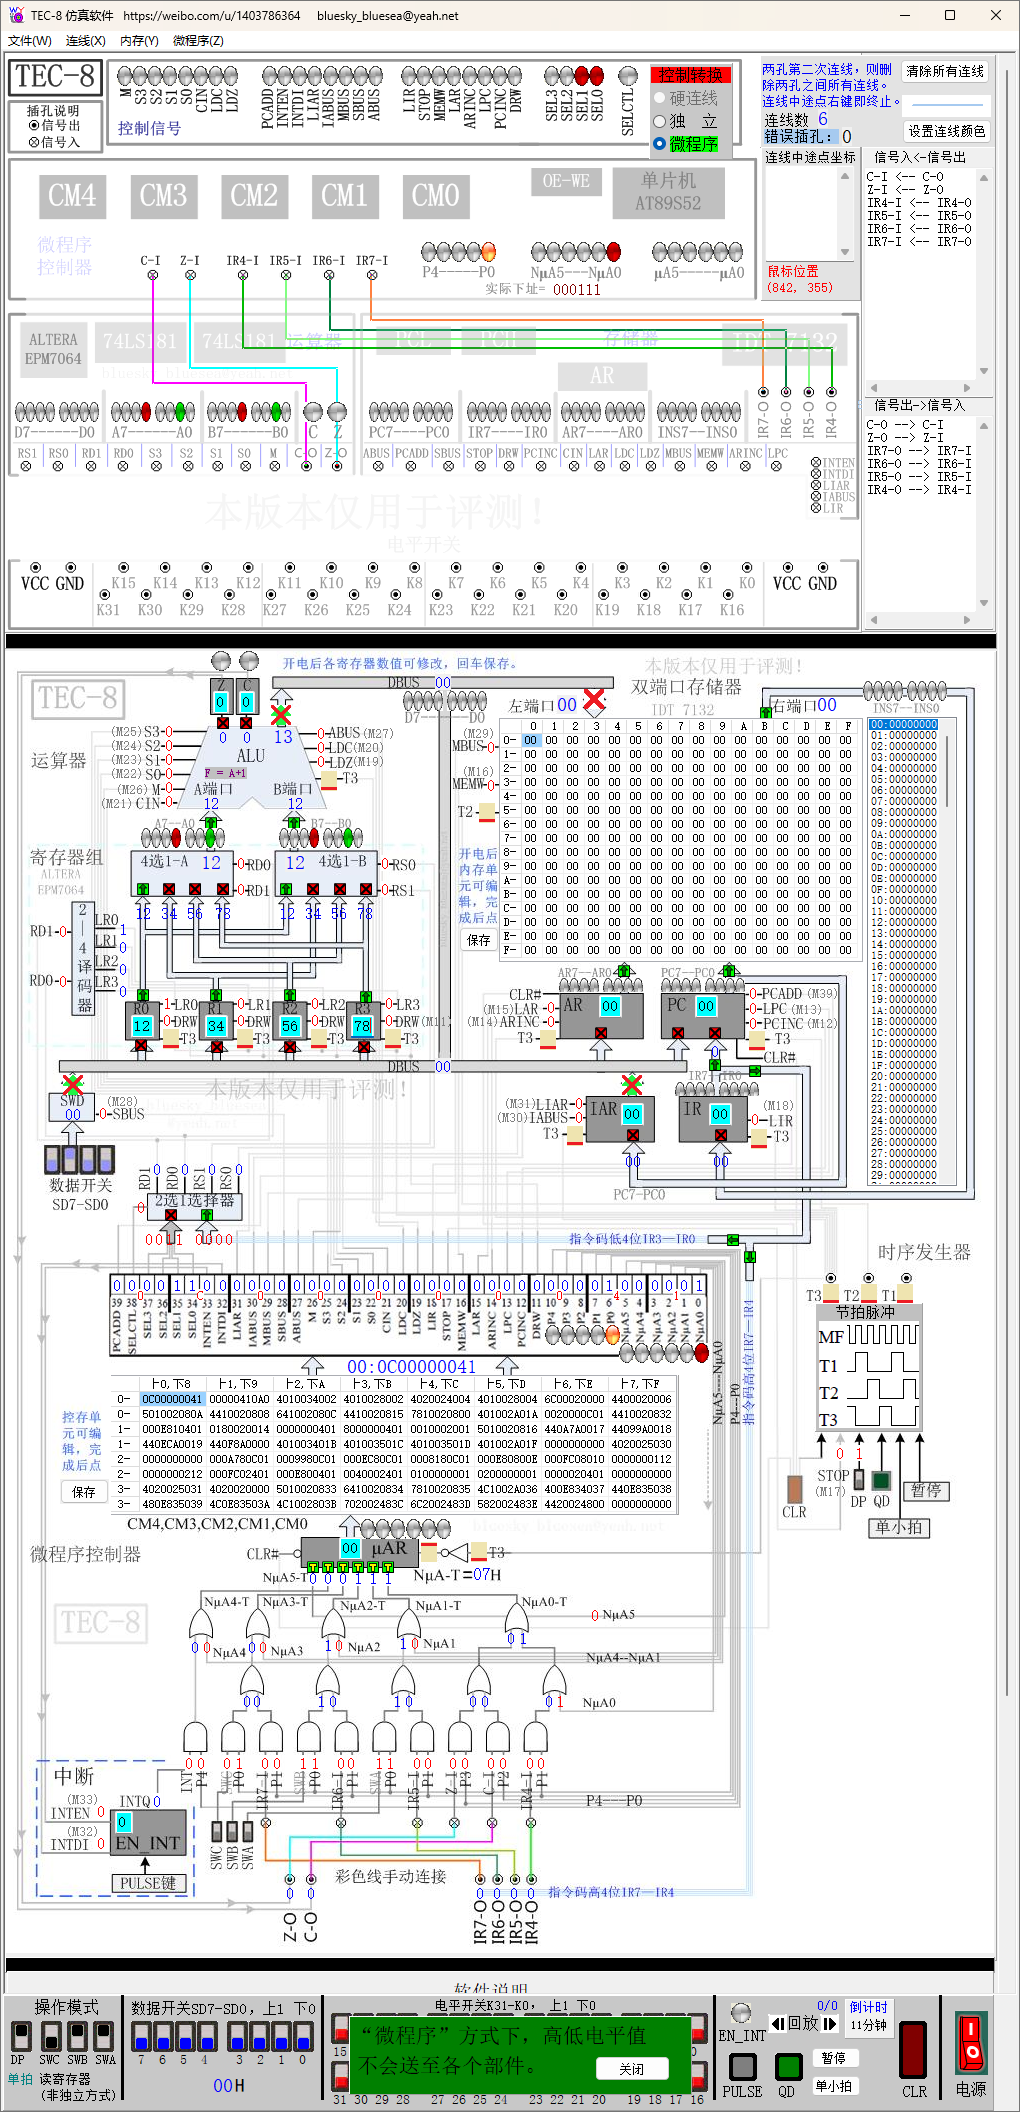
\includegraphics[width=0.3\textwidth]{screenshots/4.1.2.1.png}
    }
    \subfigure[]{
        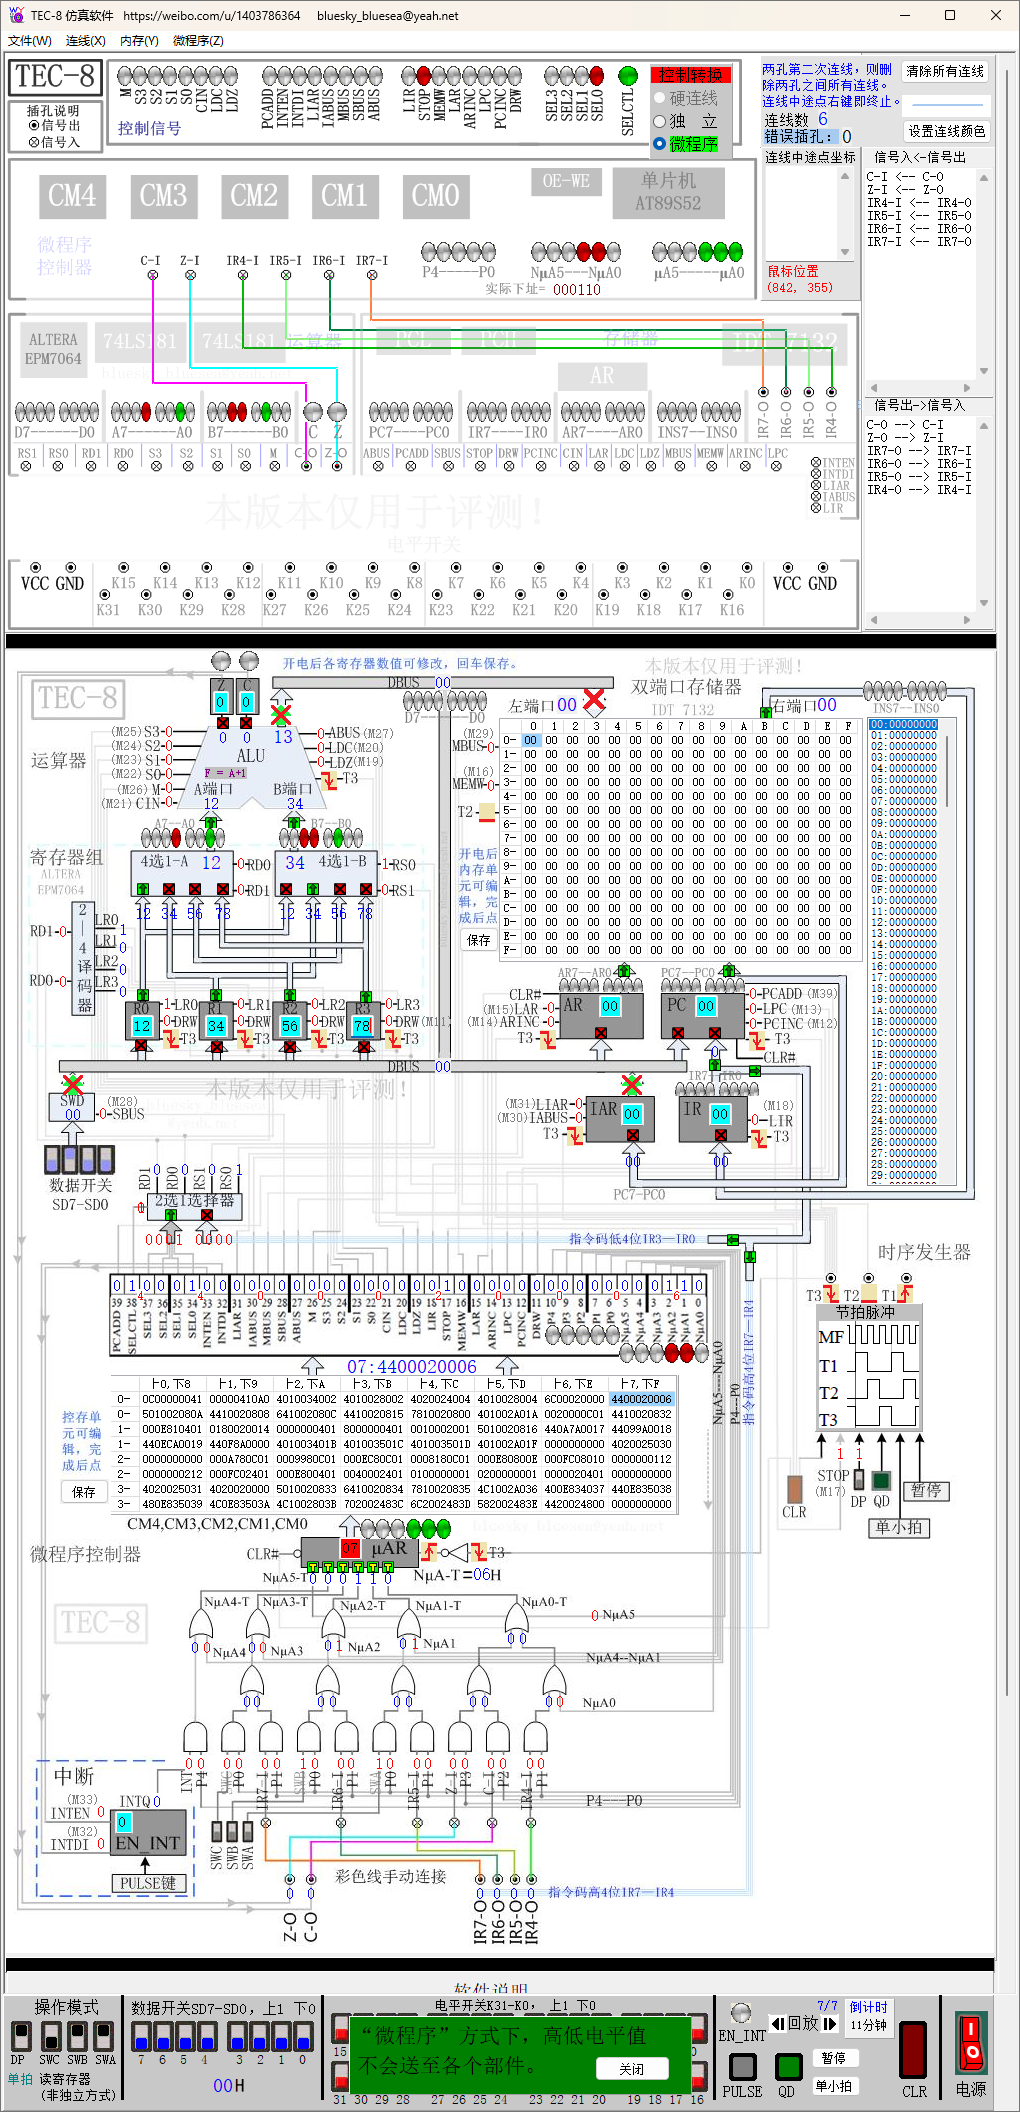
\includegraphics[width=0.3\textwidth]{screenshots/4.1.2.2.png}
    }
    \\
    \subfigure[]{
        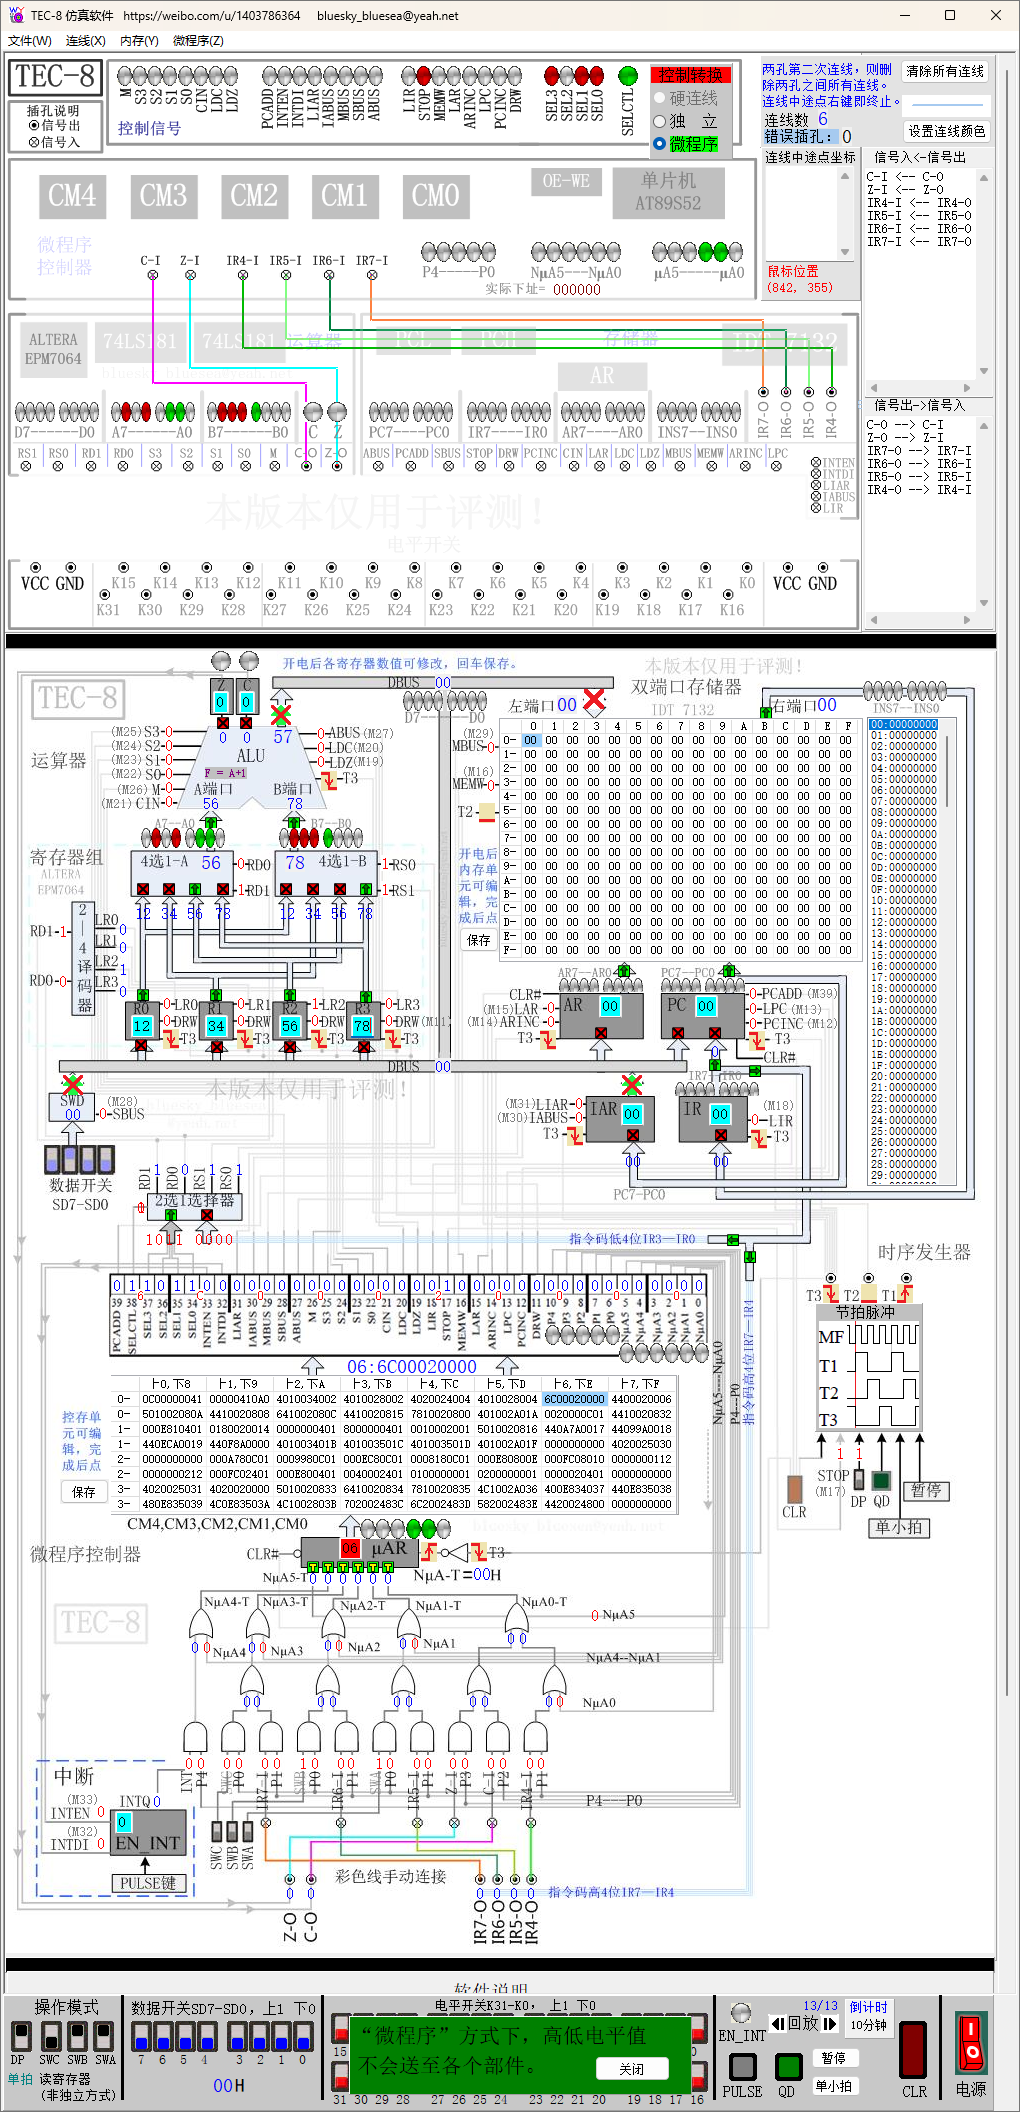
\includegraphics[width=0.3\textwidth]{screenshots/4.1.2.3.png}
    }
    \subfigure[]{
        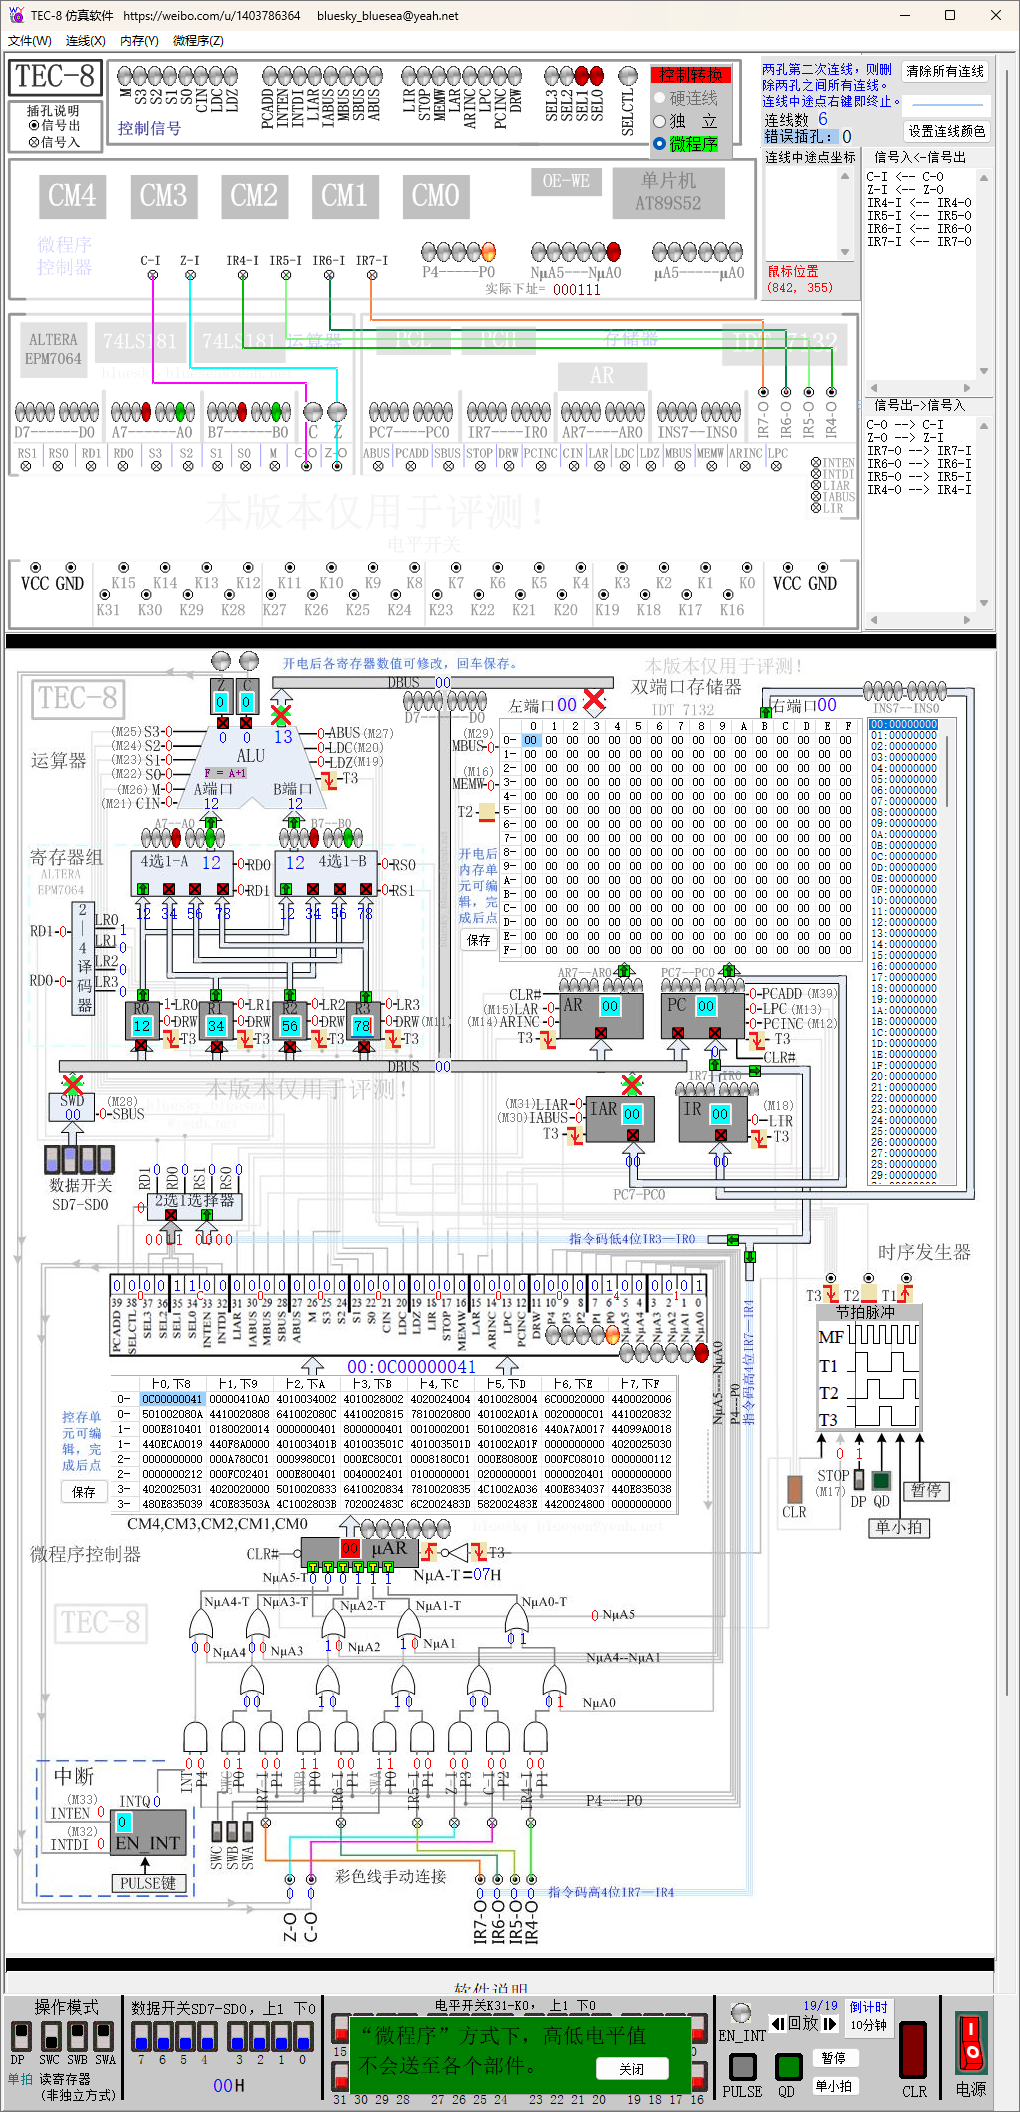
\includegraphics[width=0.3\textwidth]{screenshots/4.1.2.4.png}
    }
    \caption{读寄存器}
    \label{fig: read register}
\end{figure}

\begin{figure}[htbp]
    \centering
    \subfigure[]{
        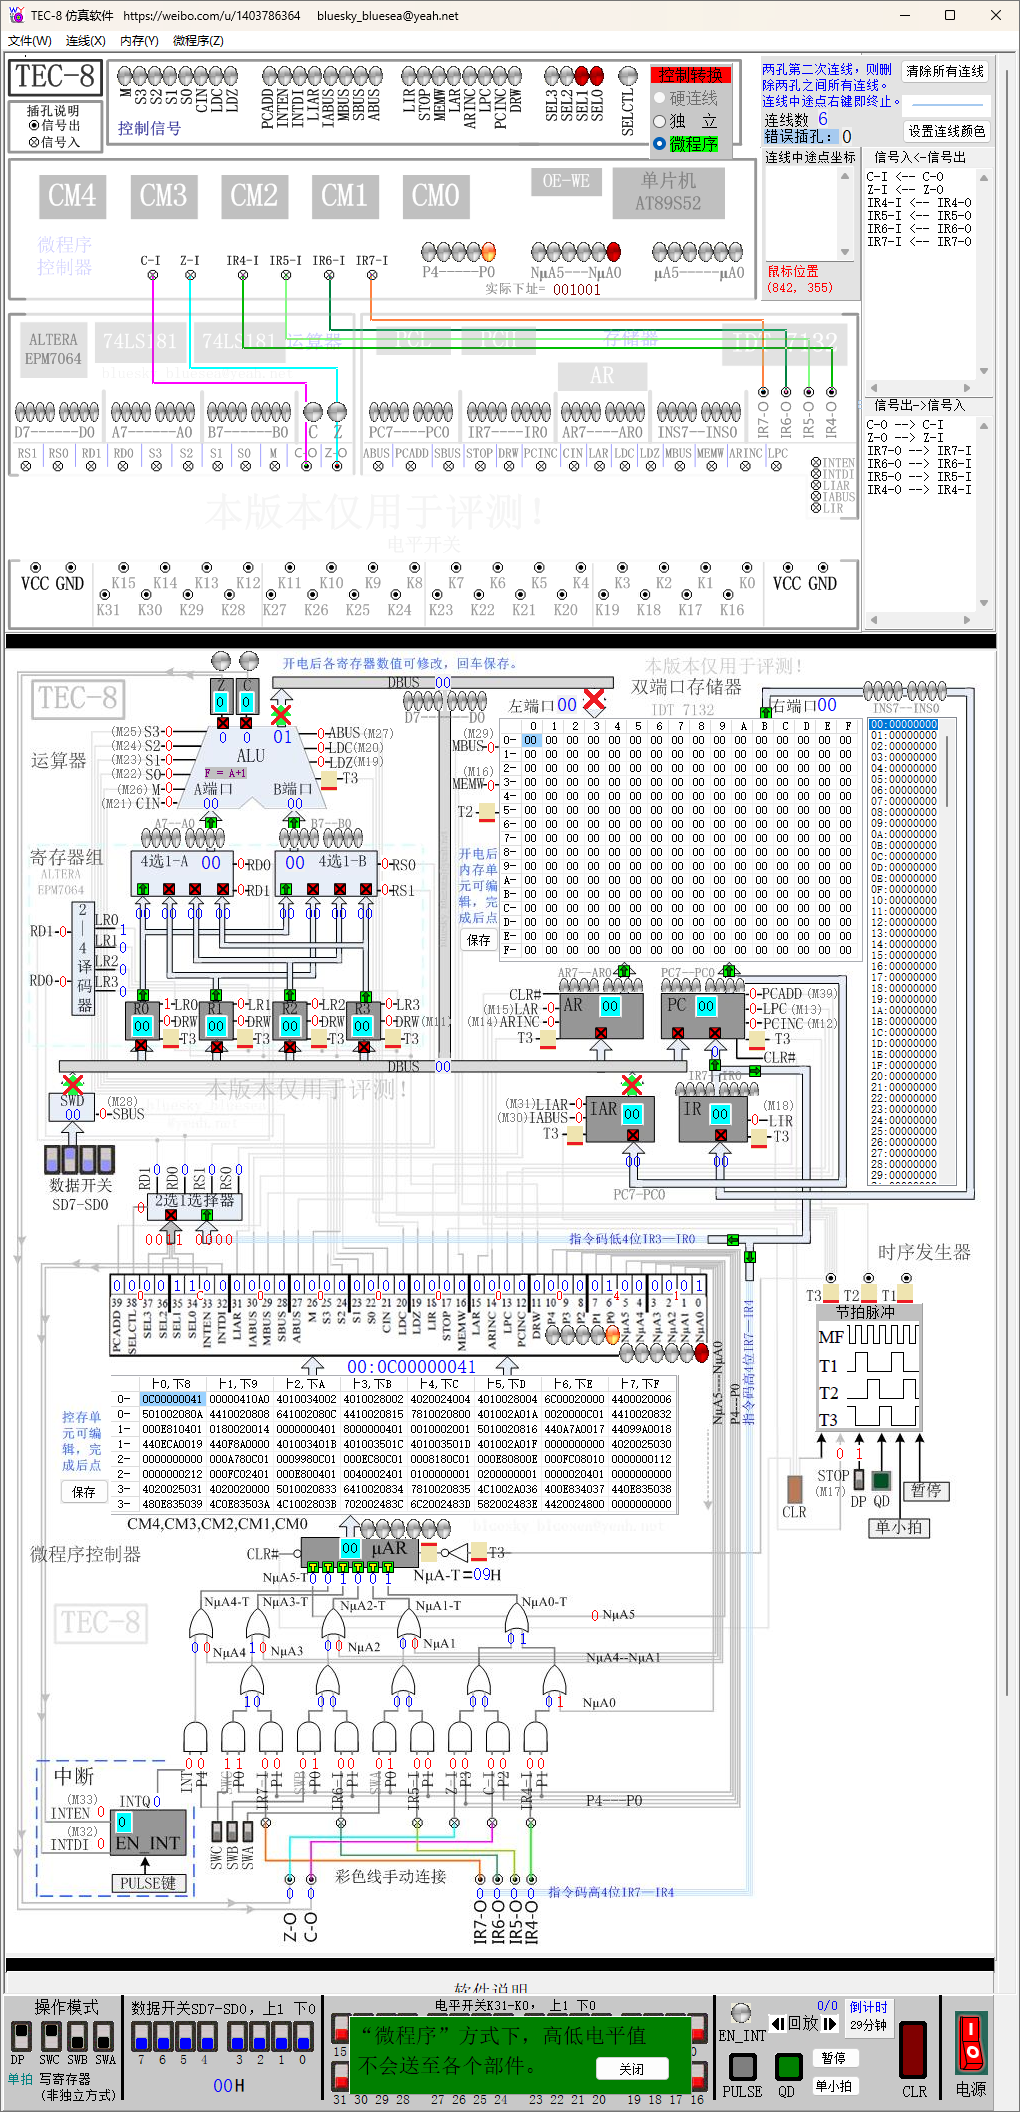
\includegraphics[width=0.3\textwidth]{screenshots/4.1.1.1.png}
    }
    \subfigure[]{
        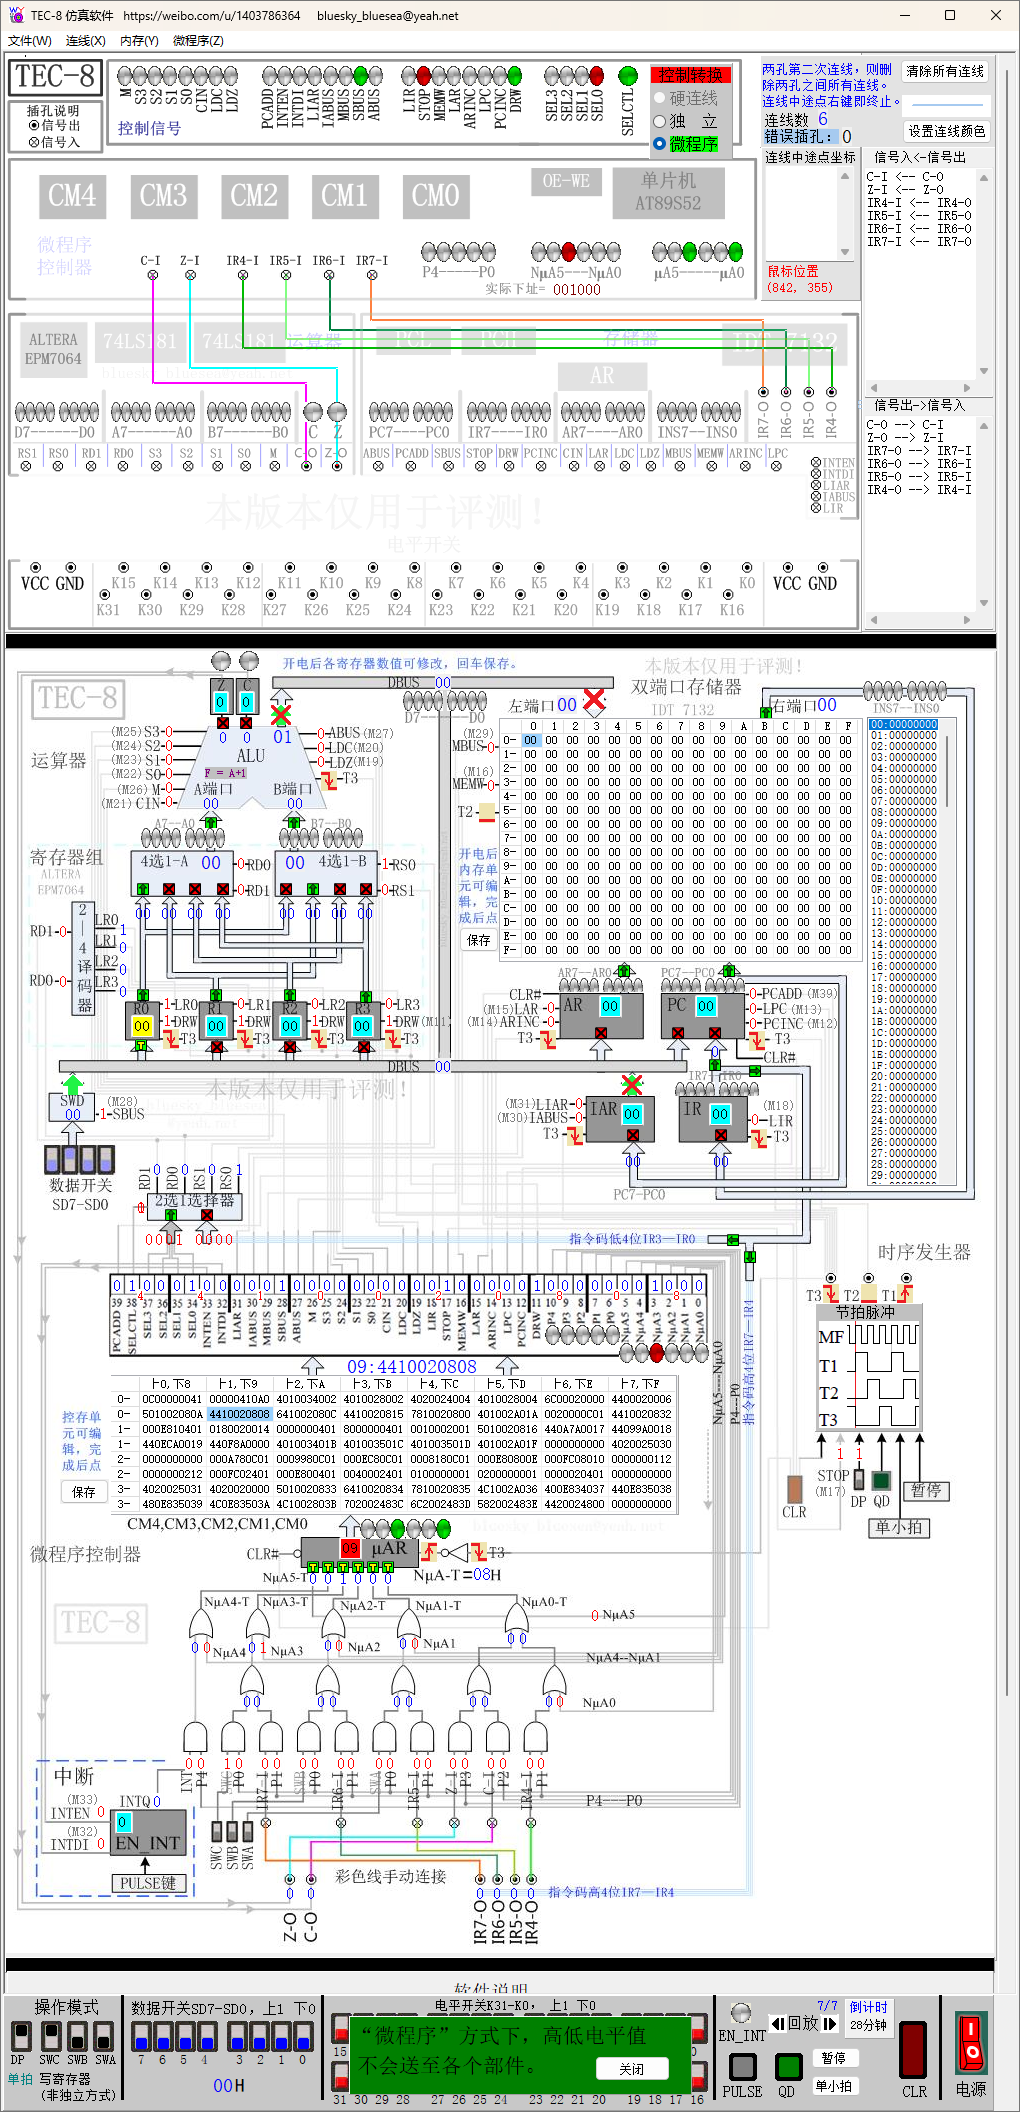
\includegraphics[width=0.3\textwidth]{screenshots/4.1.1.2.png}
    }
    \subfigure[]{
        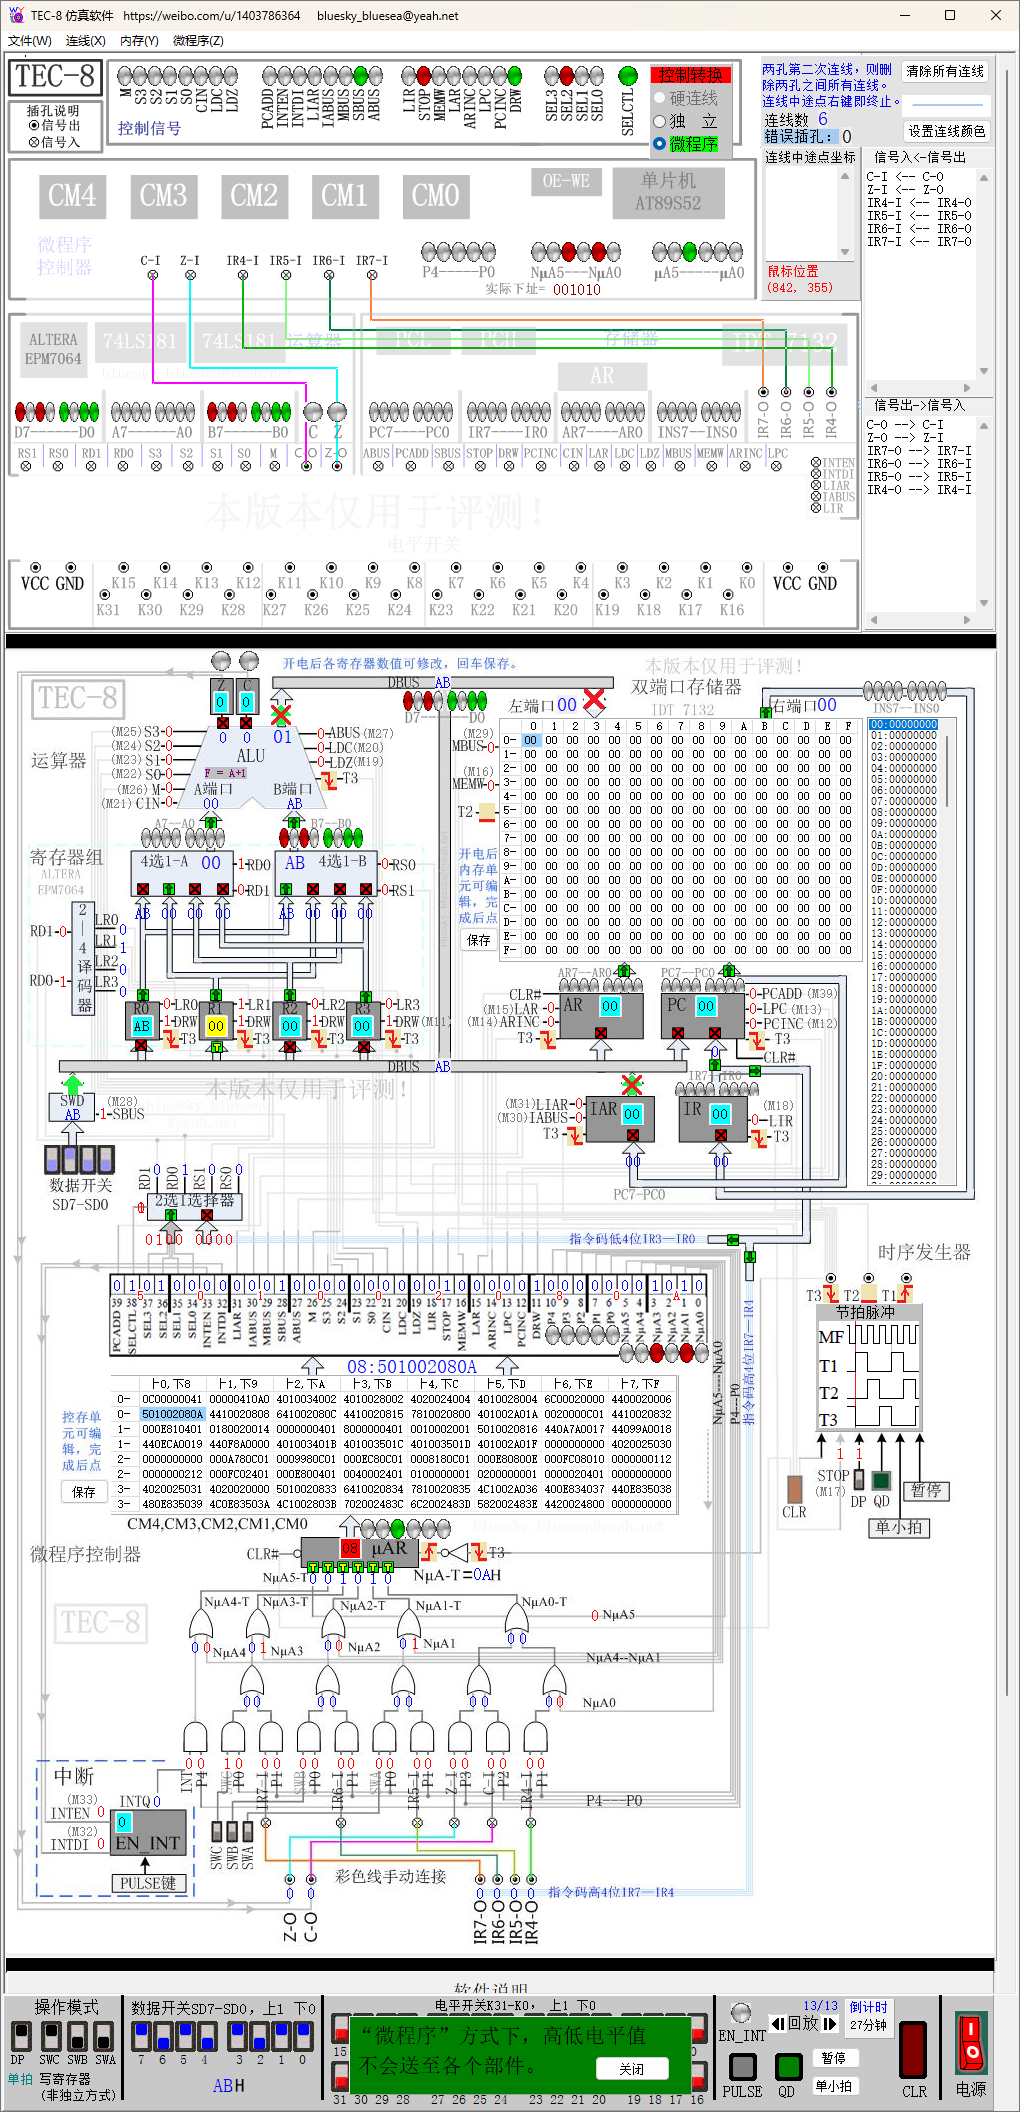
\includegraphics[width=0.3\textwidth]{screenshots/4.1.1.3.png}
    }
    \\
    \subfigure[]{
        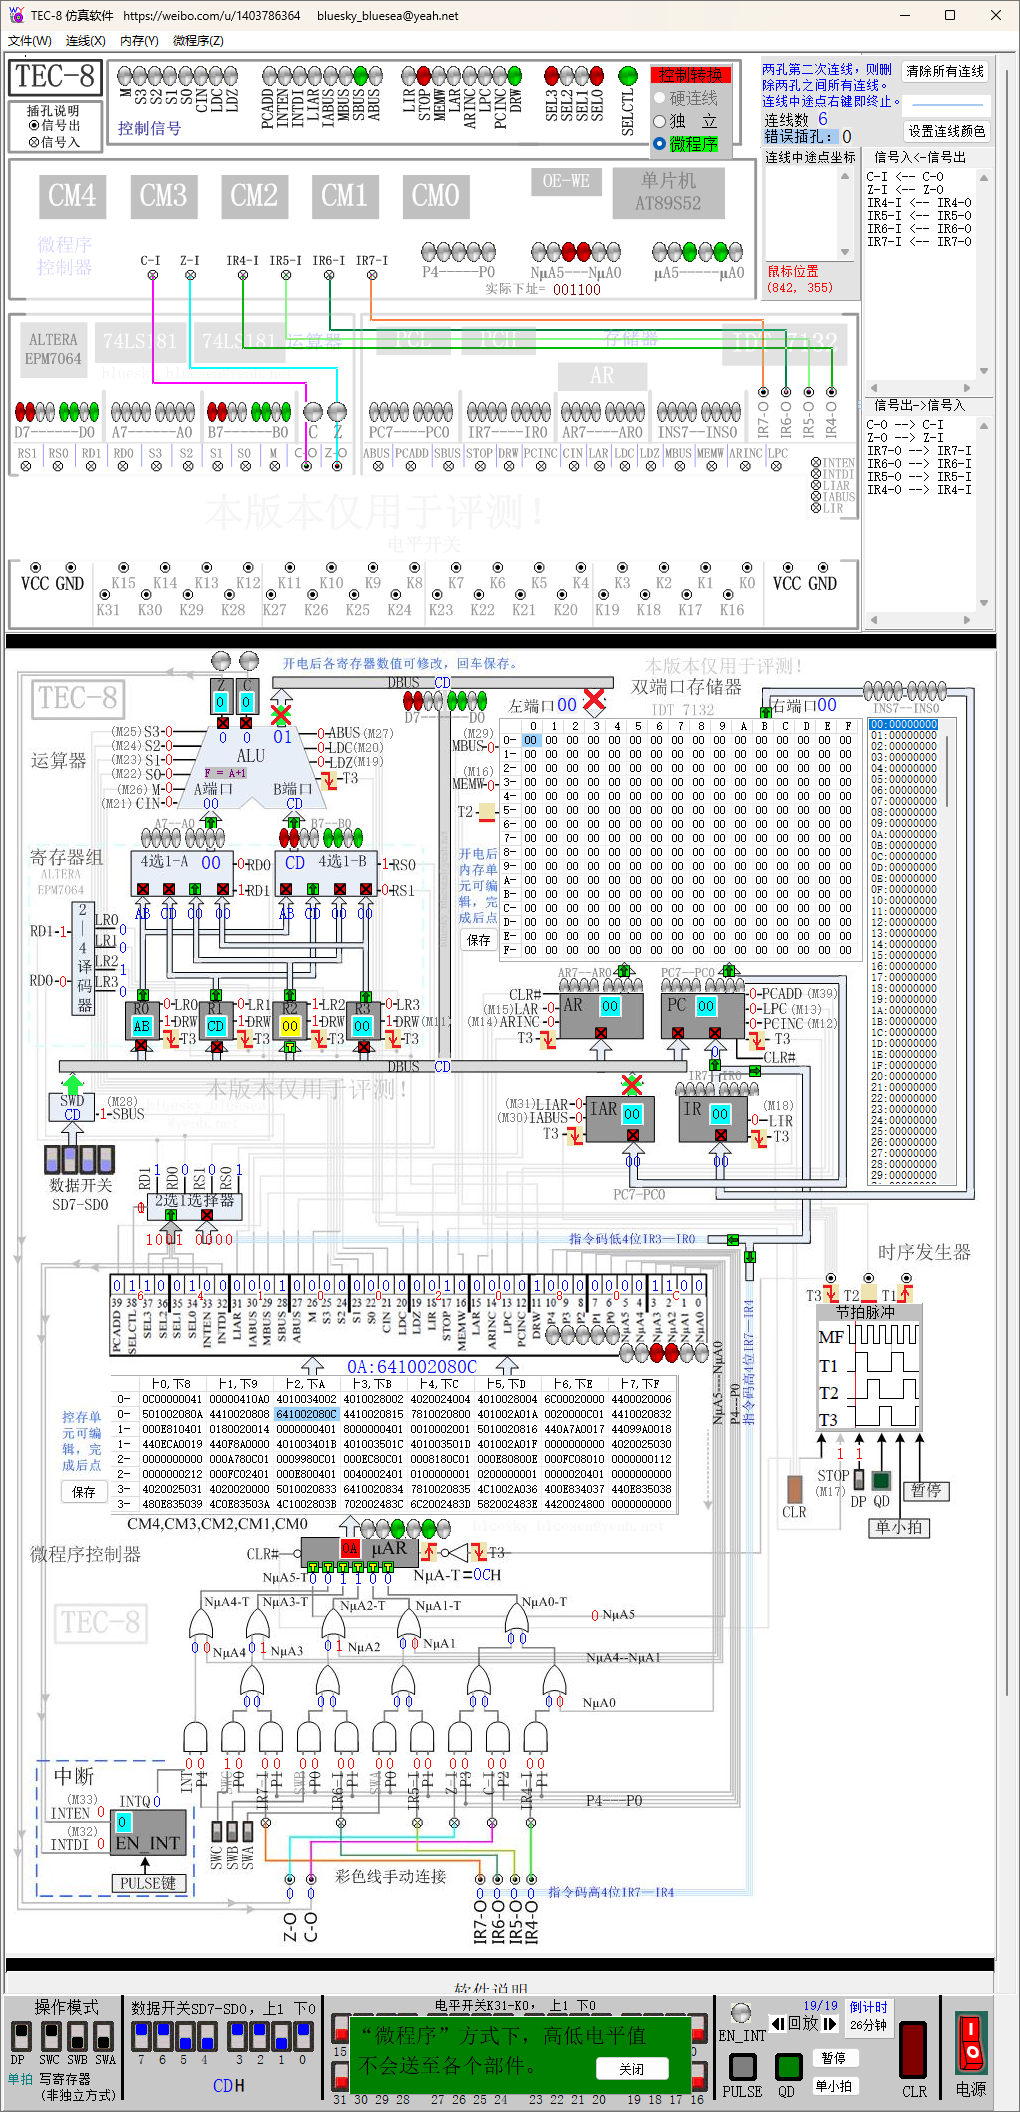
\includegraphics[width=0.3\textwidth]{screenshots/4.1.1.4.png}
    }
    \subfigure[]{
        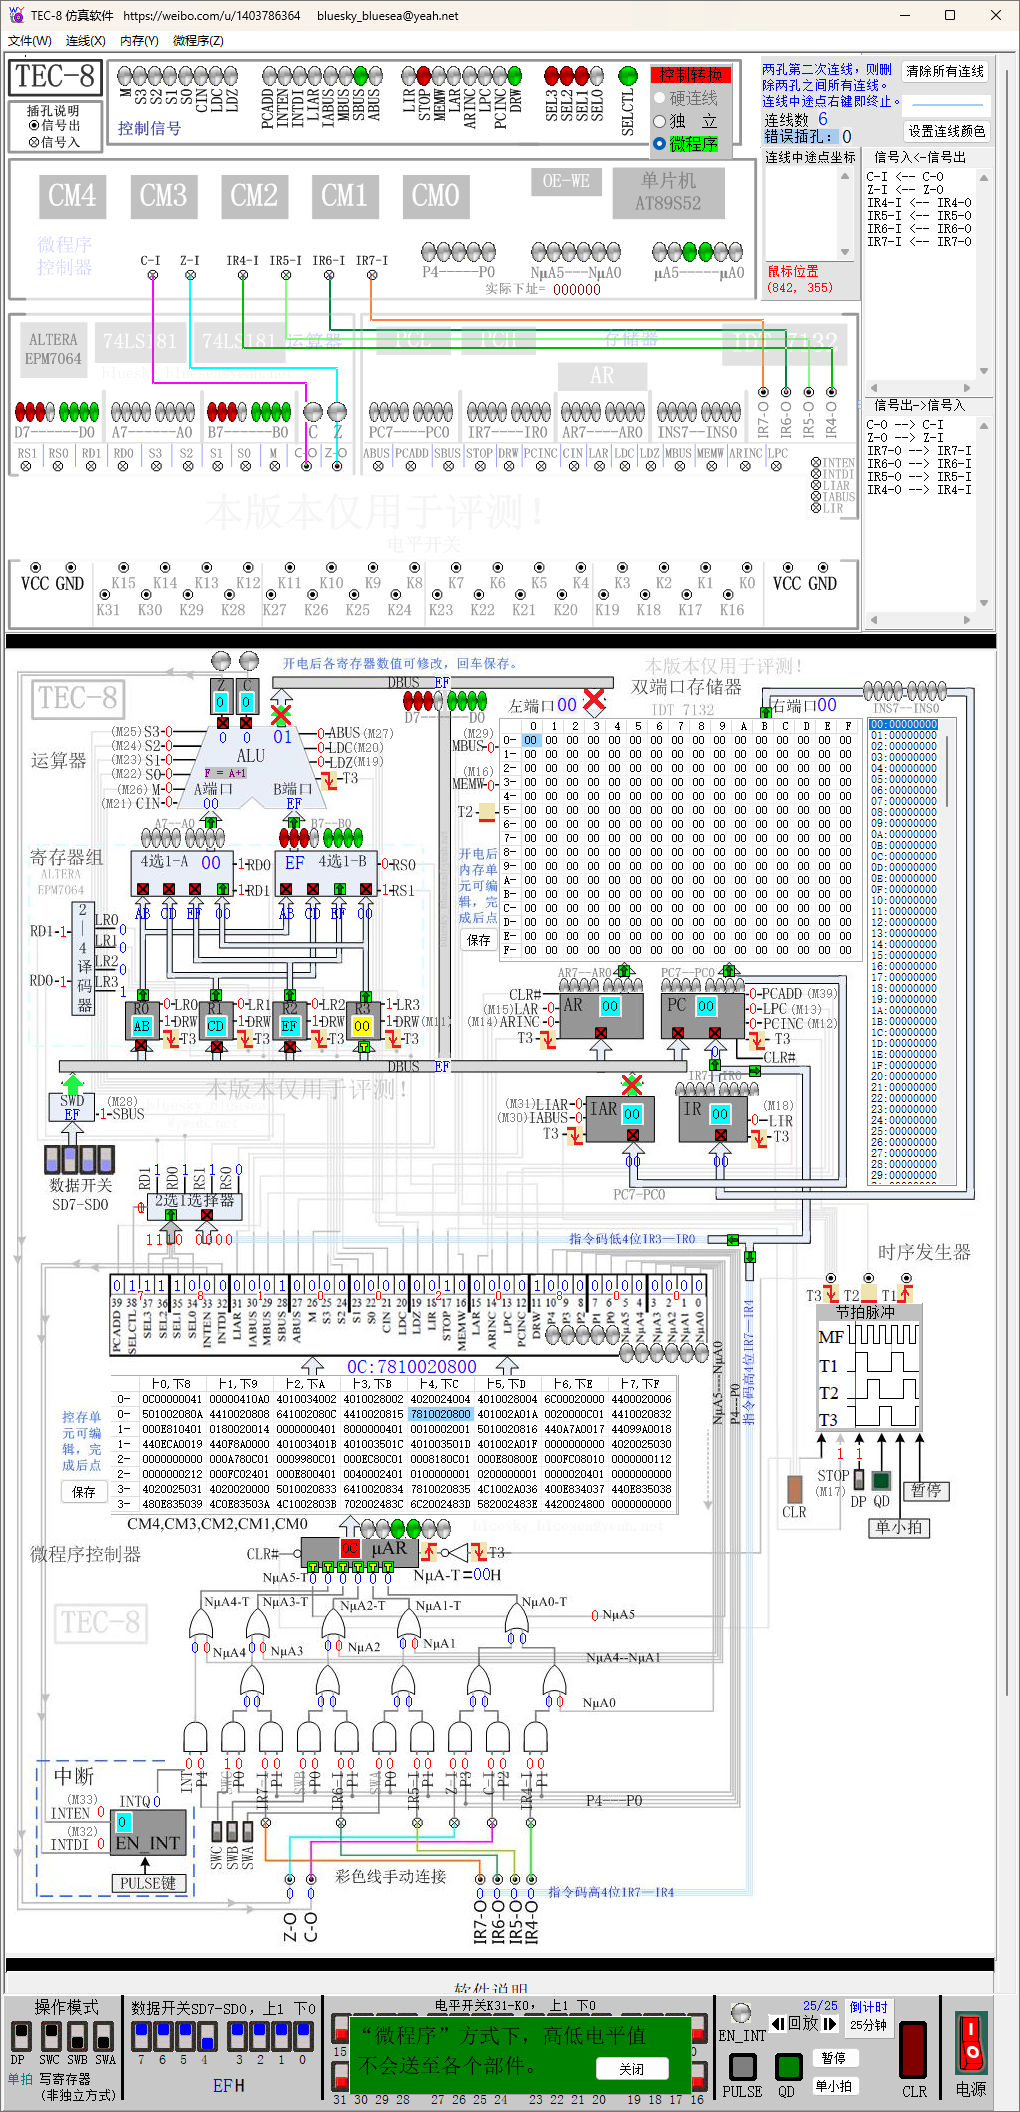
\includegraphics[width=0.3\textwidth]{screenshots/4.1.1.5.png}
    }
    \subfigure[]{
        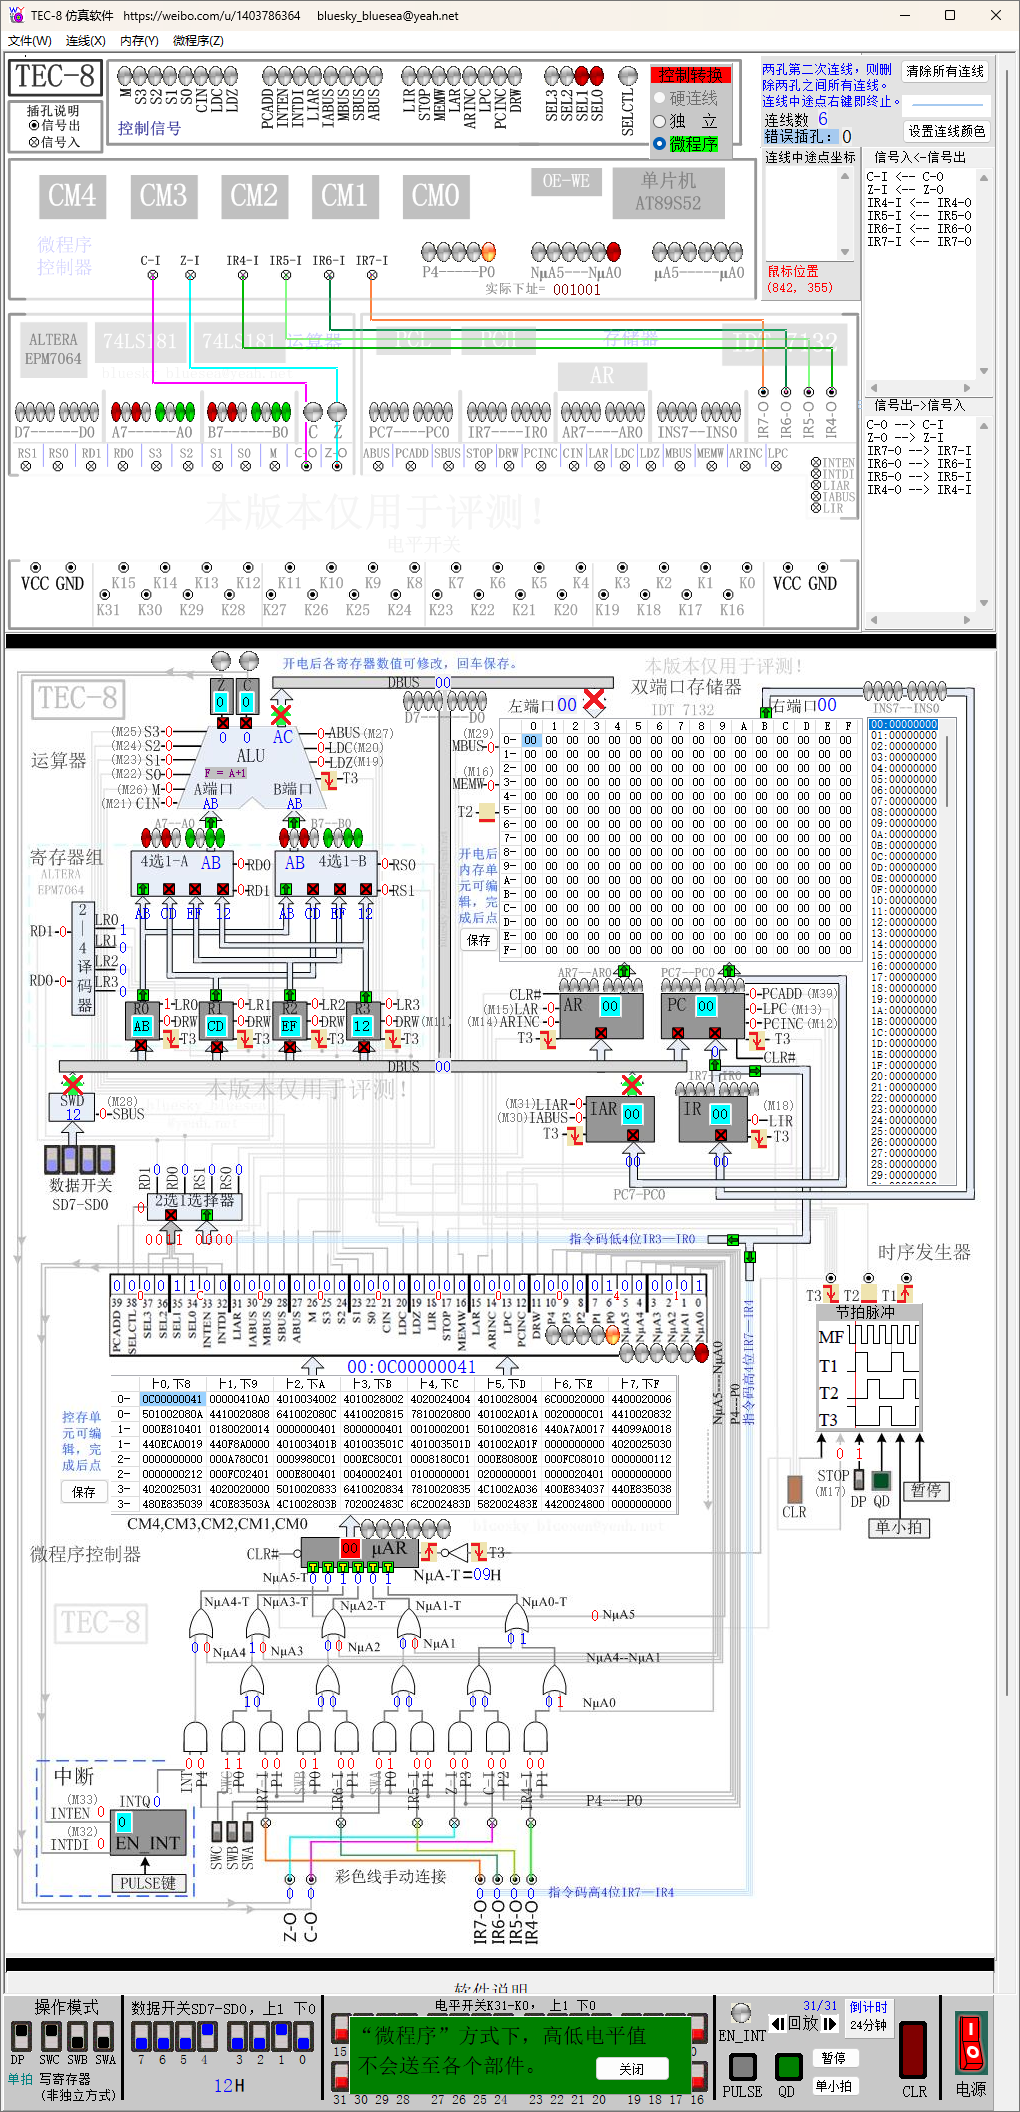
\includegraphics[width=0.3\textwidth]{screenshots/4.1.1.6.png}
    }
    \caption{写寄存器}
    \label{fig: write register}
\end{figure}

\begin{figure}[htbp]
    \centering
    \subfigure[]{
        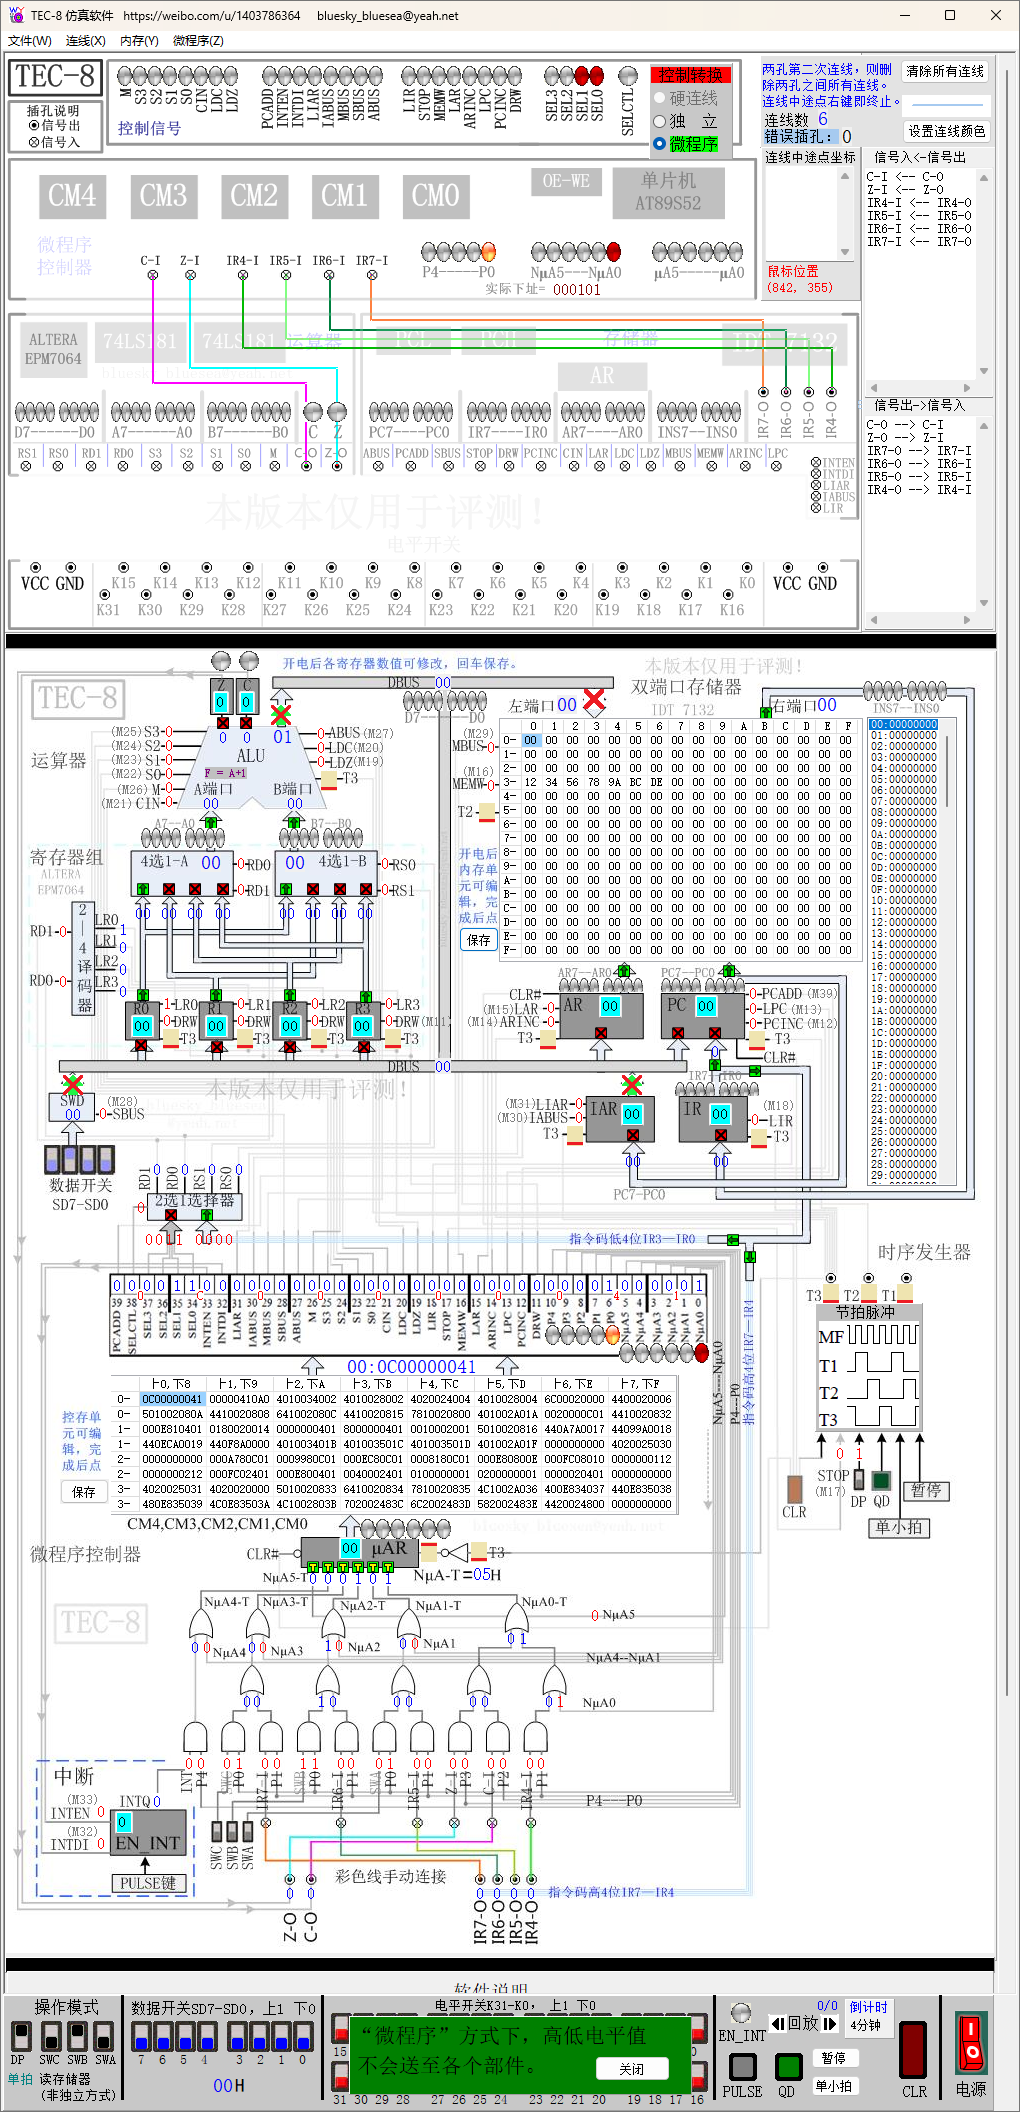
\includegraphics[width=0.3\textwidth]{screenshots/4.1.4.1.png}
    }
    \subfigure[]{
        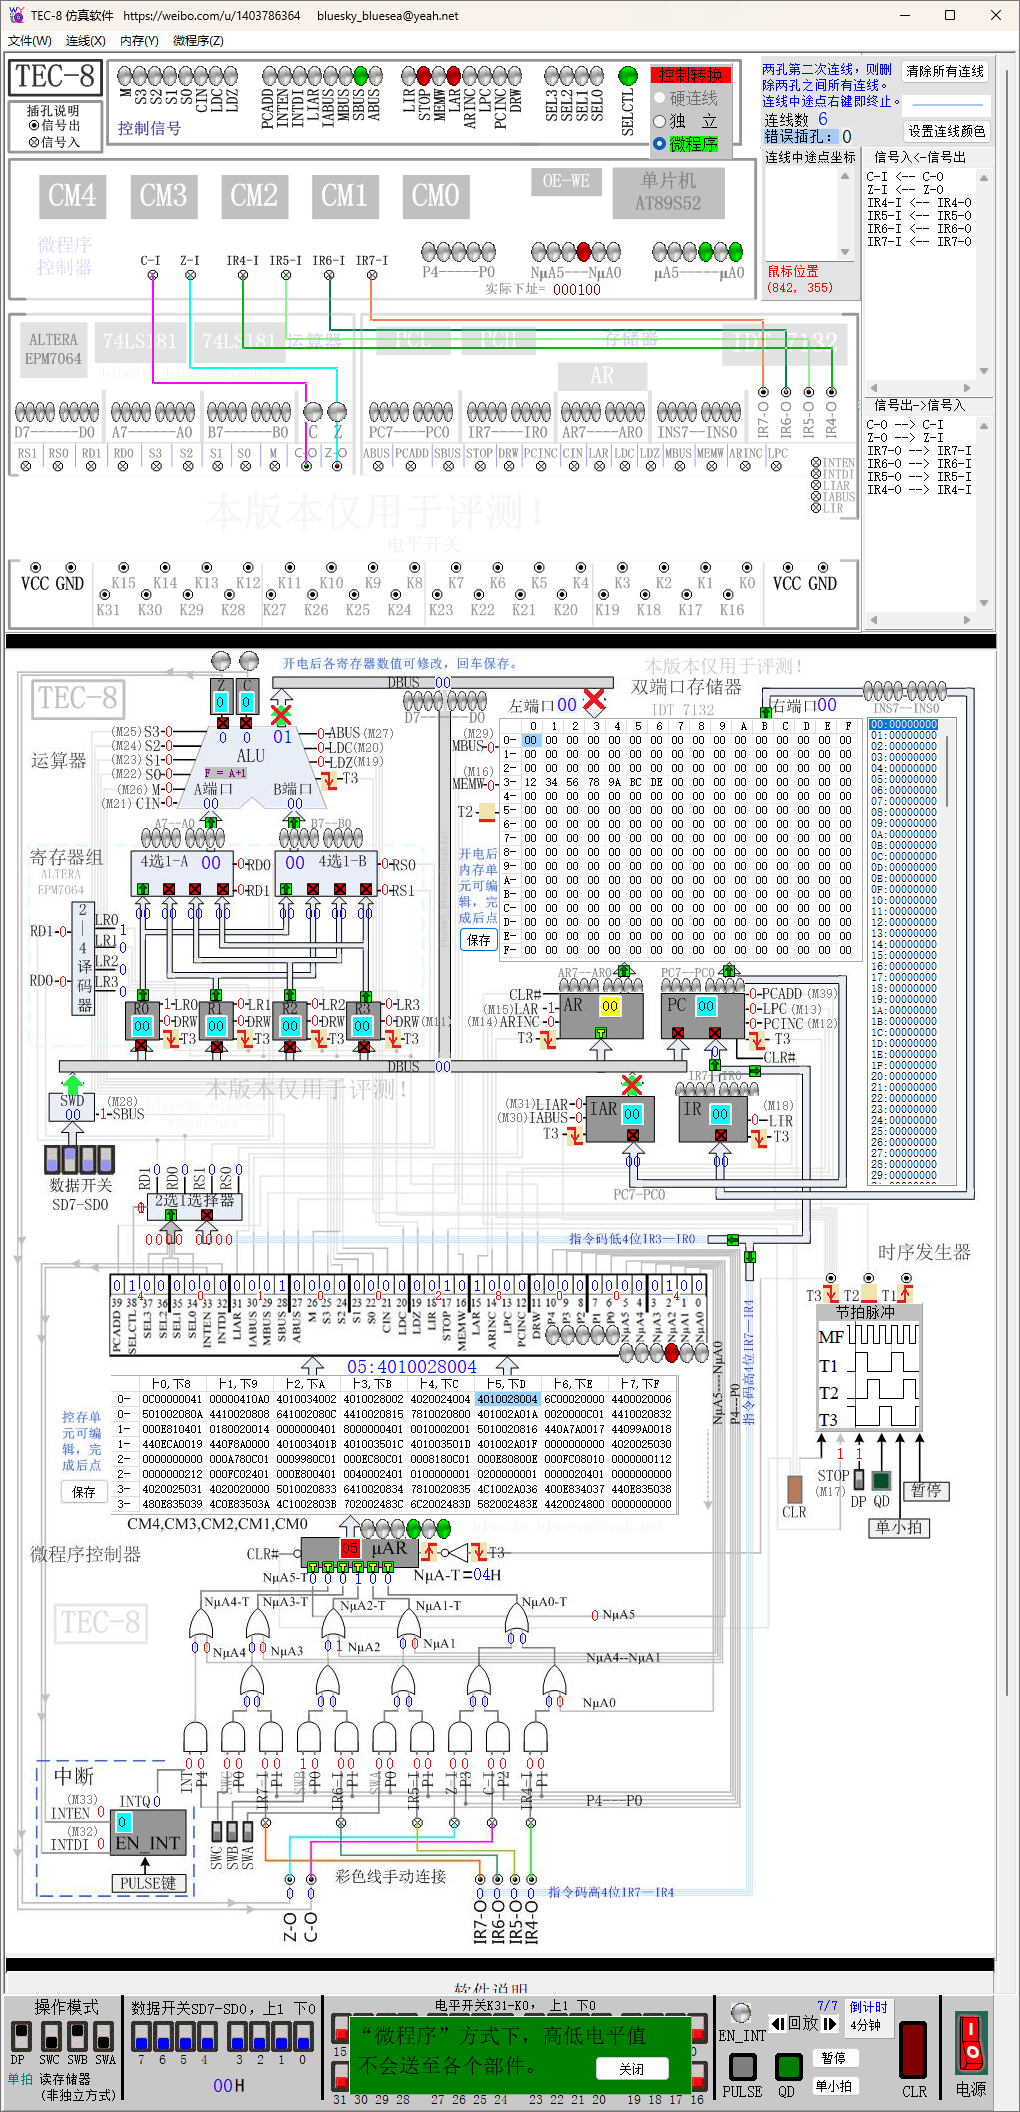
\includegraphics[width=0.3\textwidth]{screenshots/4.1.4.2.png}
    }
    \\
    \subfigure[]{
        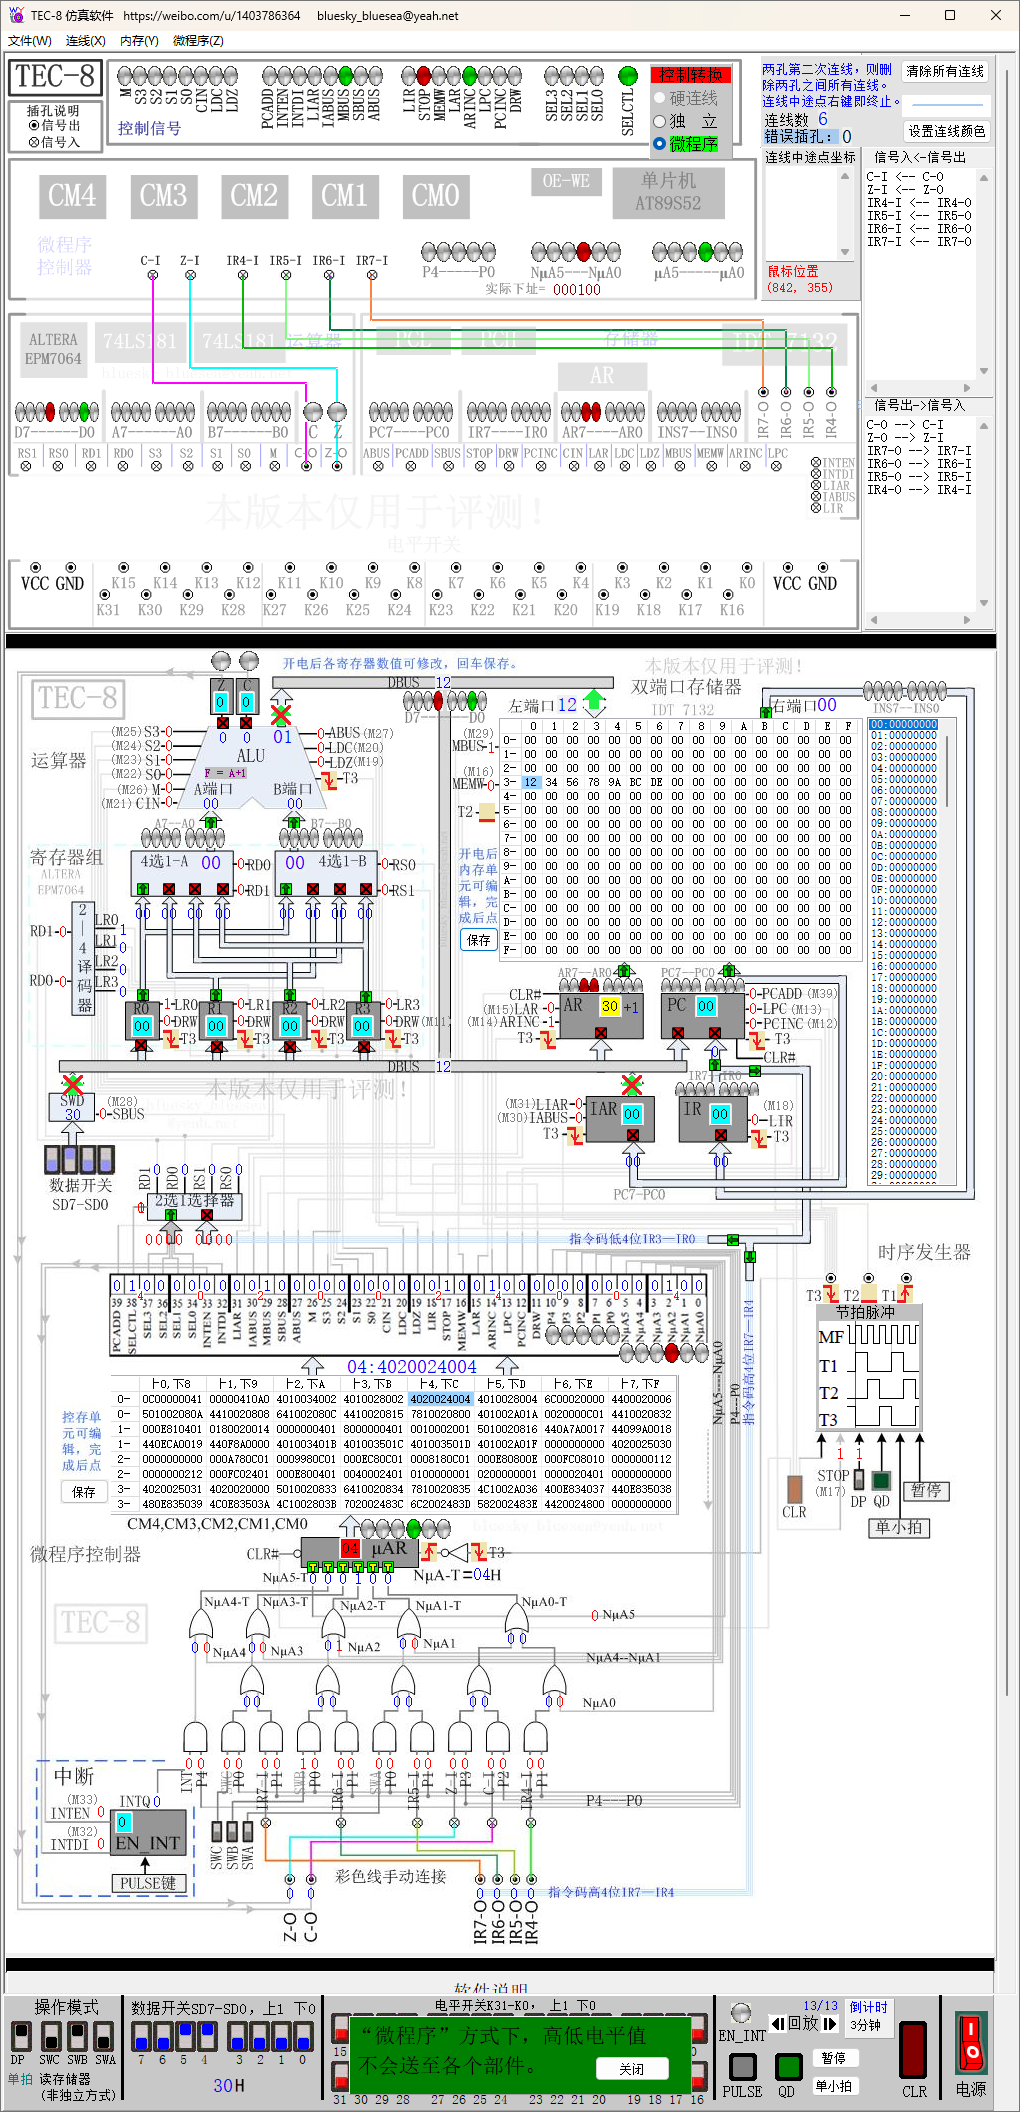
\includegraphics[width=0.3\textwidth]{screenshots/4.1.4.3.png}
    }
    \subfigure[]{
        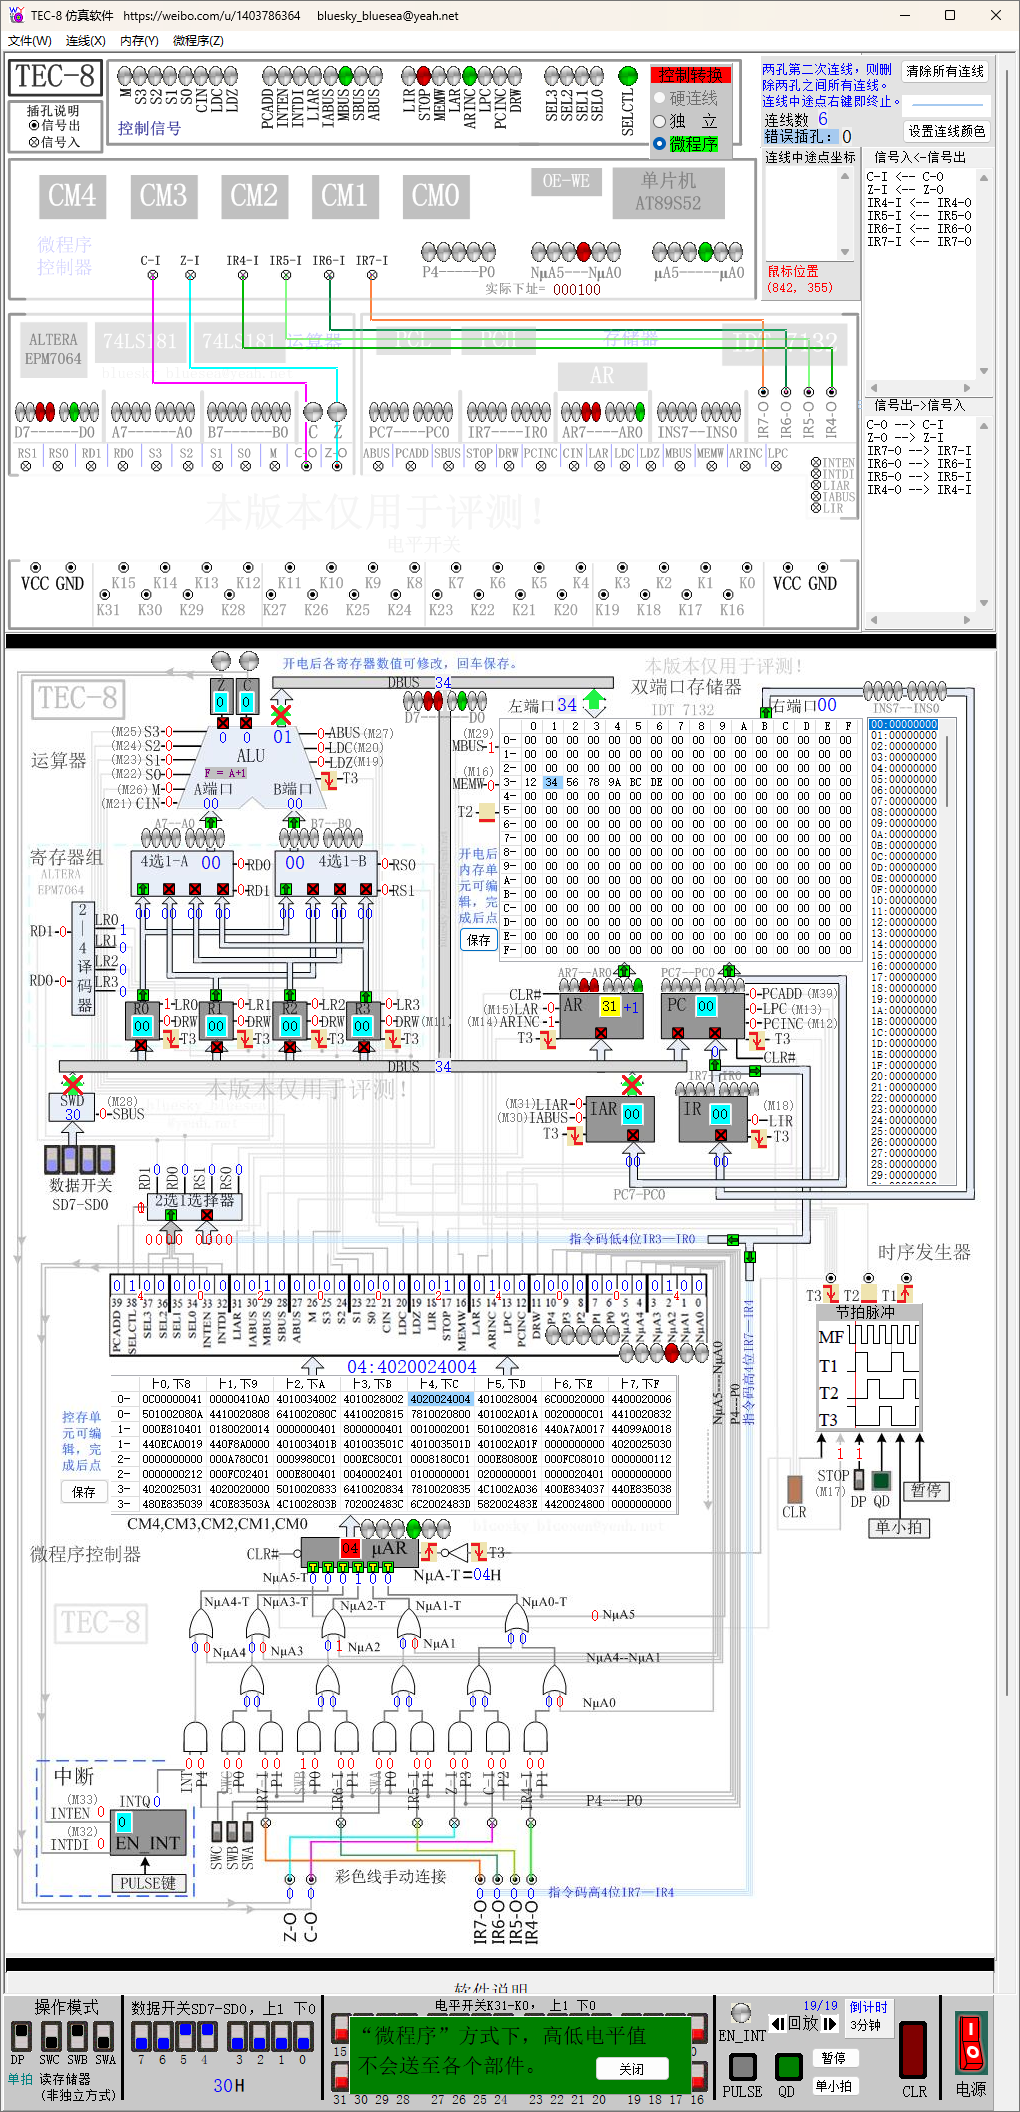
\includegraphics[width=0.3\textwidth]{screenshots/4.1.4.4.png}
    }
    \caption{读存储器}
    \label{fig: read memory}
\end{figure}

\begin{figure}[htbp]
    \centering
    \subfigure[]{
        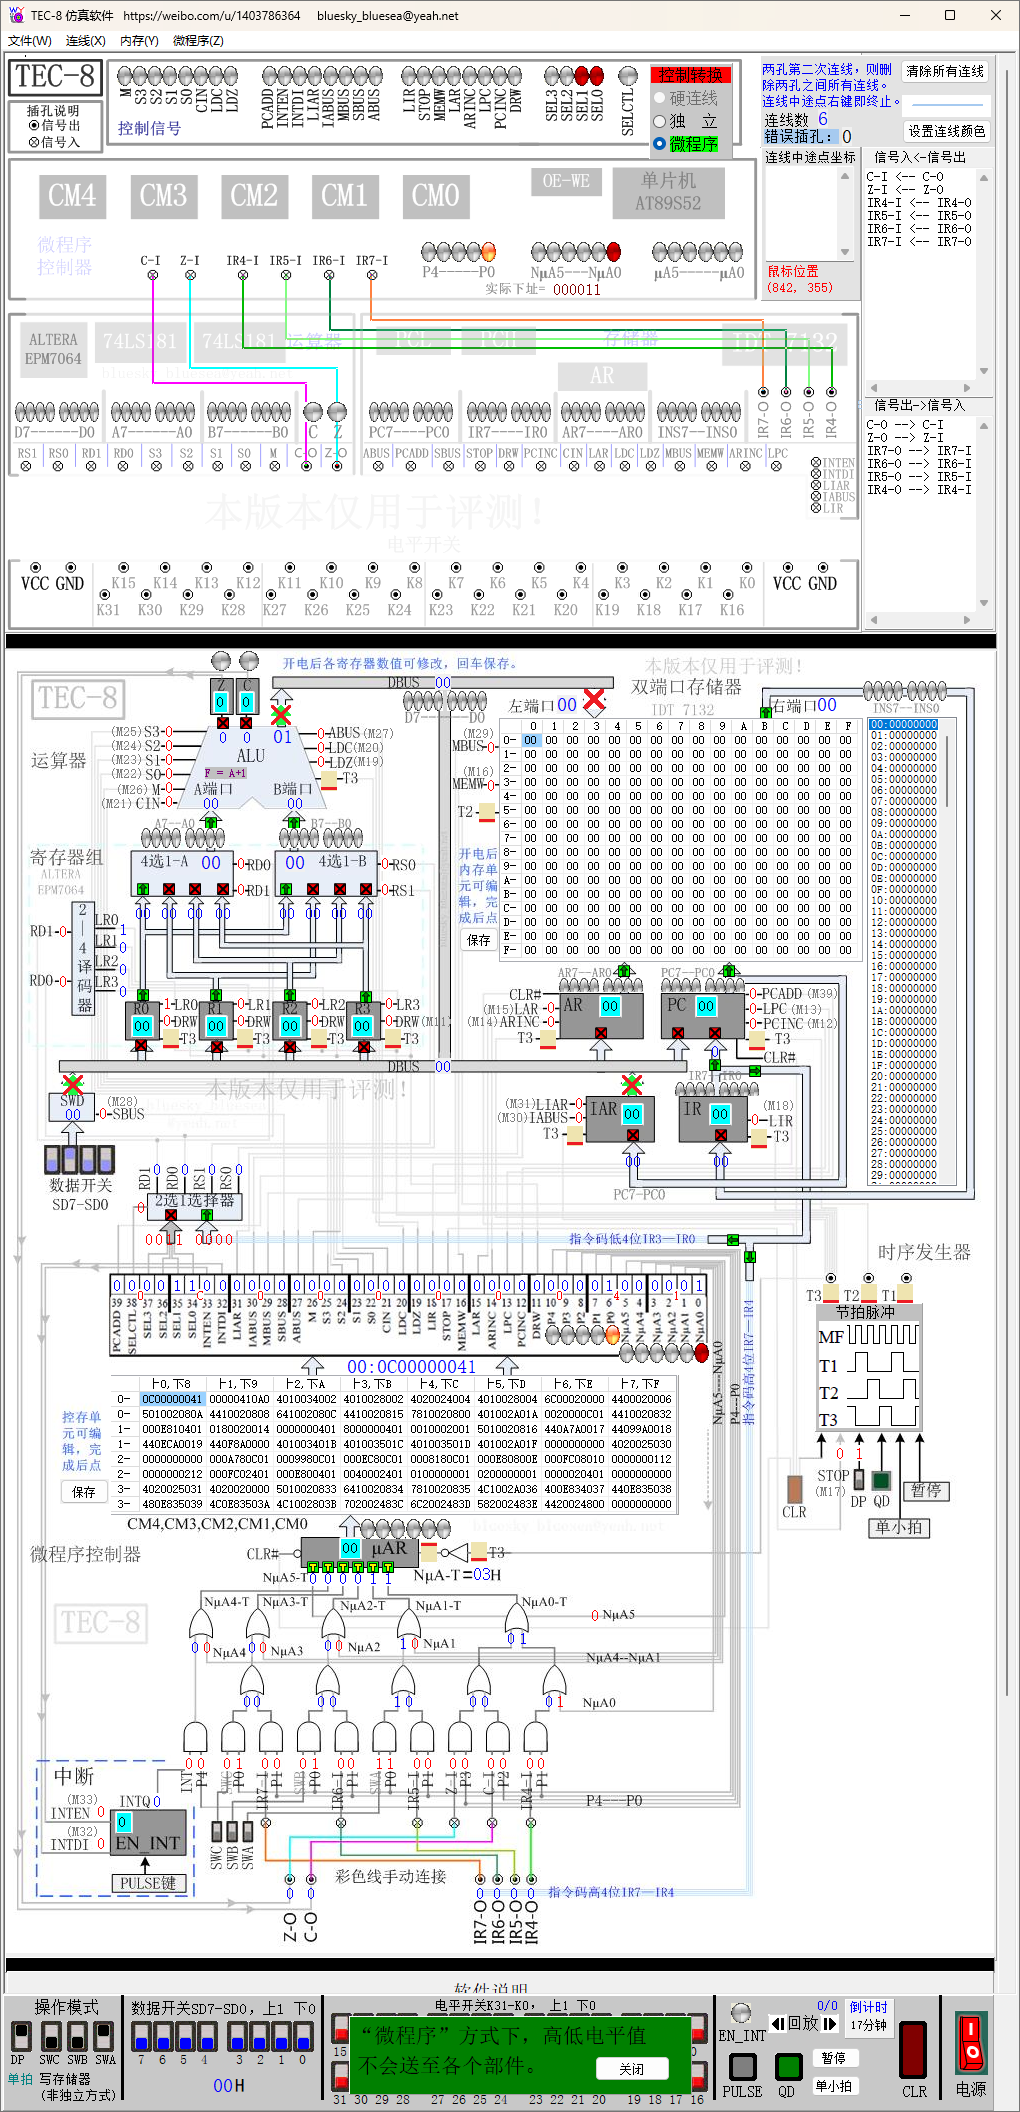
\includegraphics[width=0.3\textwidth]{screenshots/4.1.3.1.png}
    }
    \subfigure[]{
        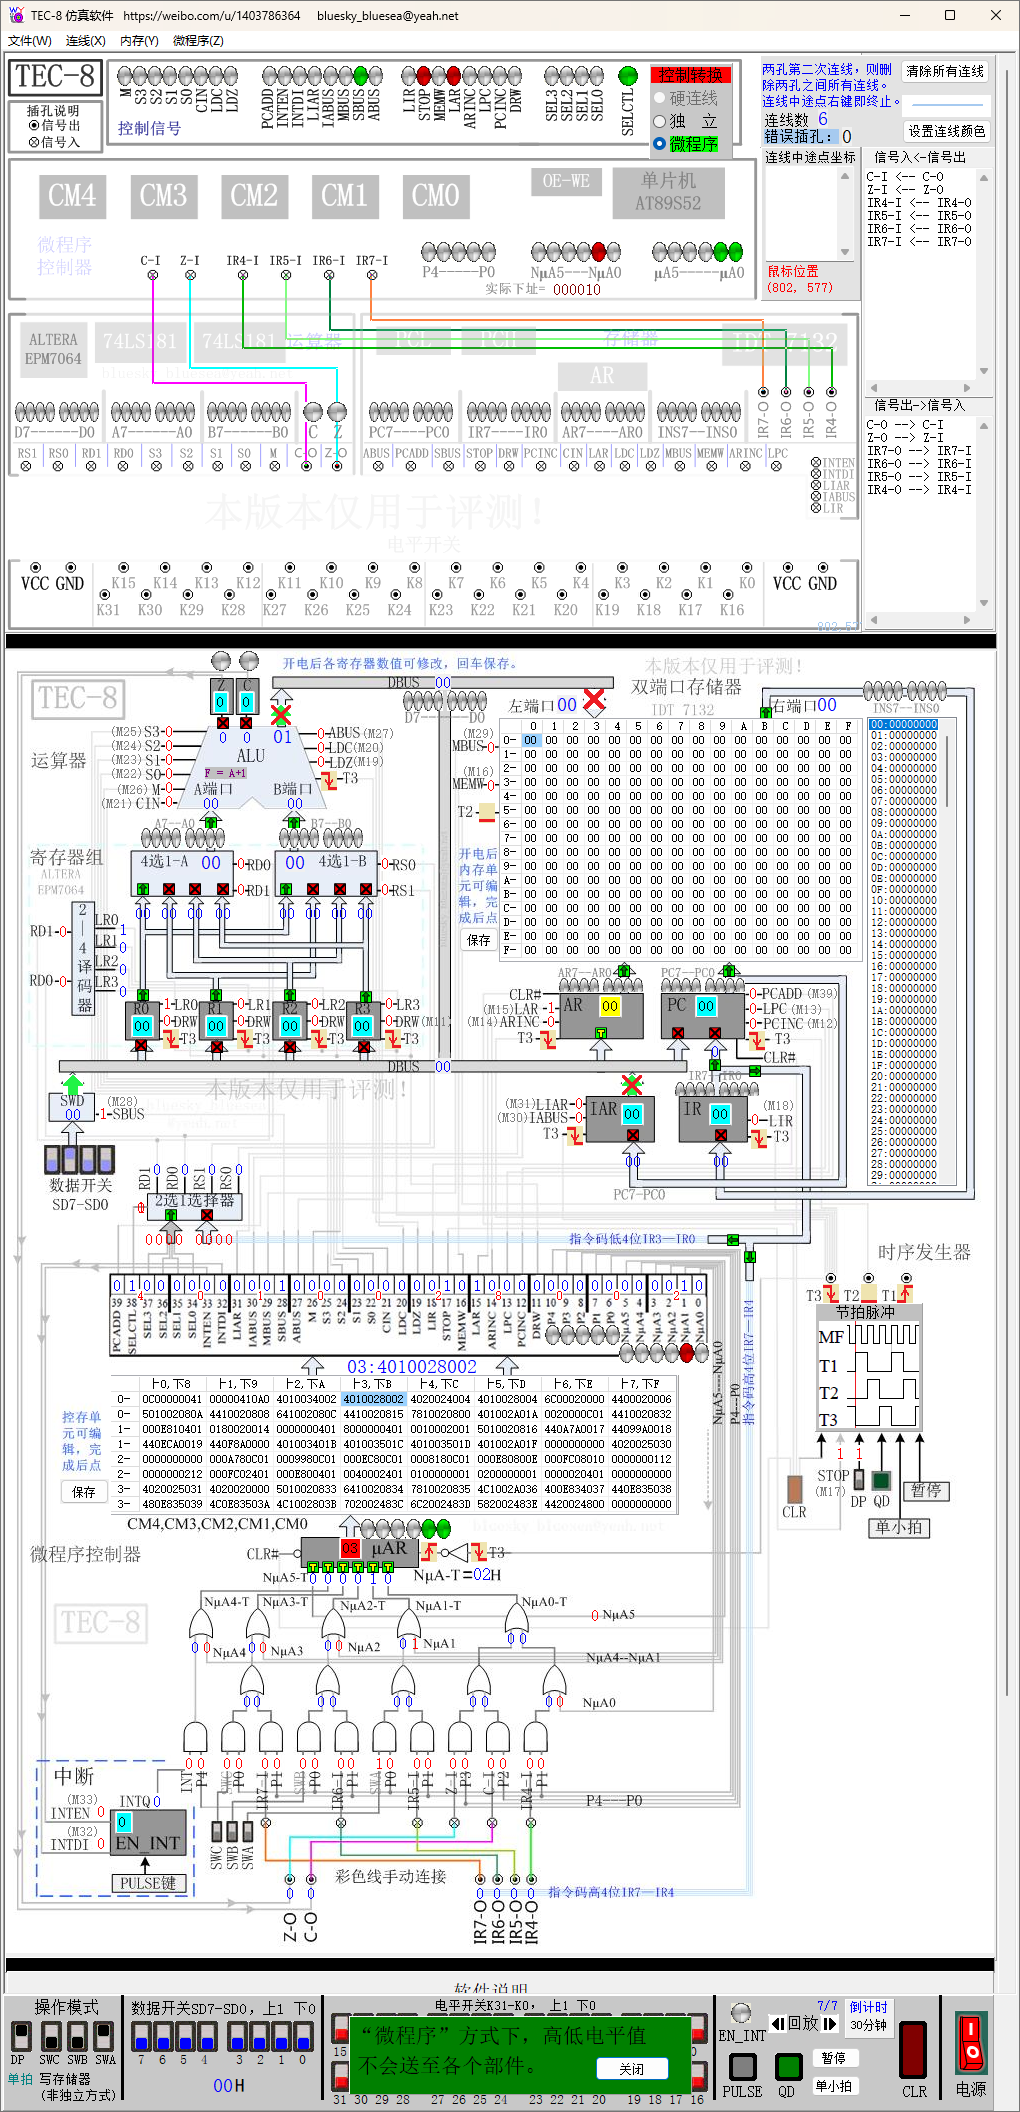
\includegraphics[width=0.3\textwidth]{screenshots/4.1.3.5.png}
    }
    \\
    \subfigure[]{
        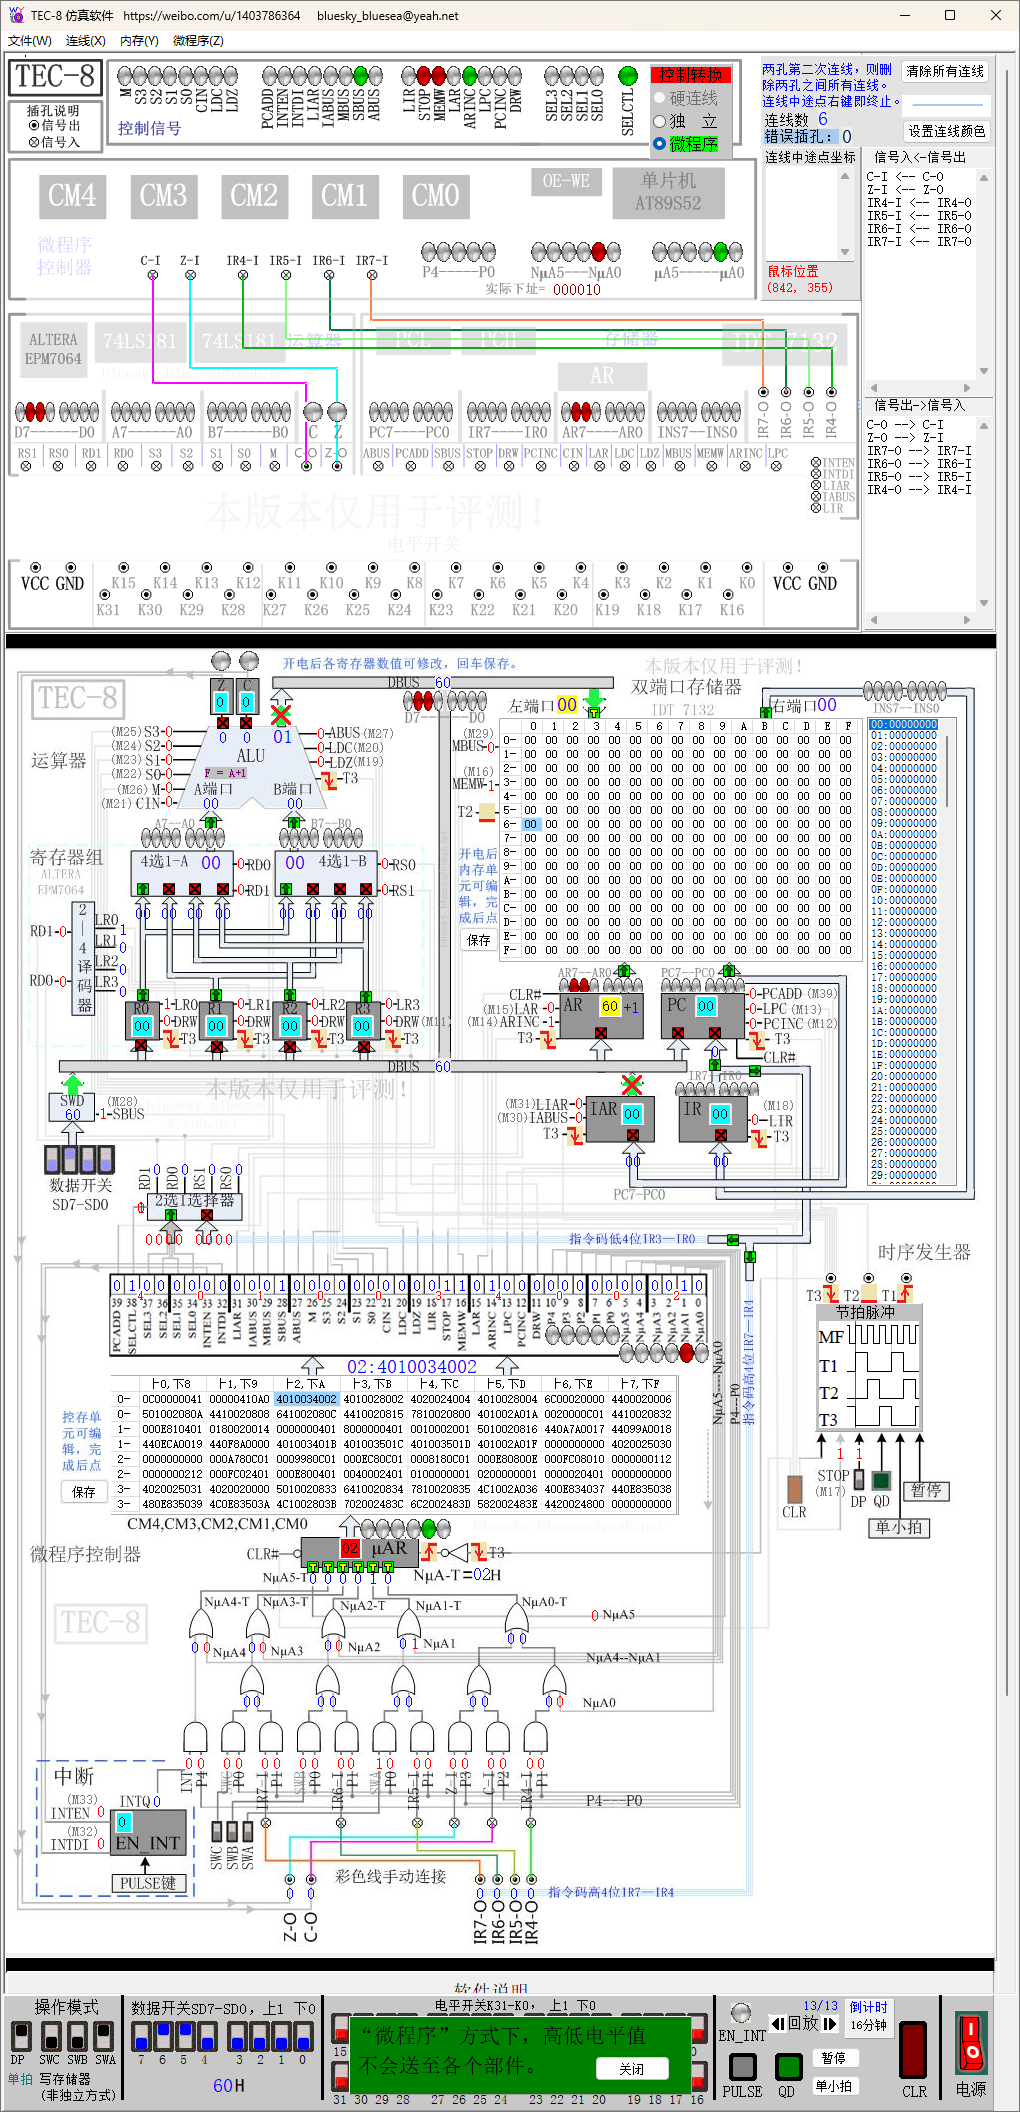
\includegraphics[width=0.3\textwidth]{screenshots/4.1.3.2.png}
    }
    \subfigure[]{
        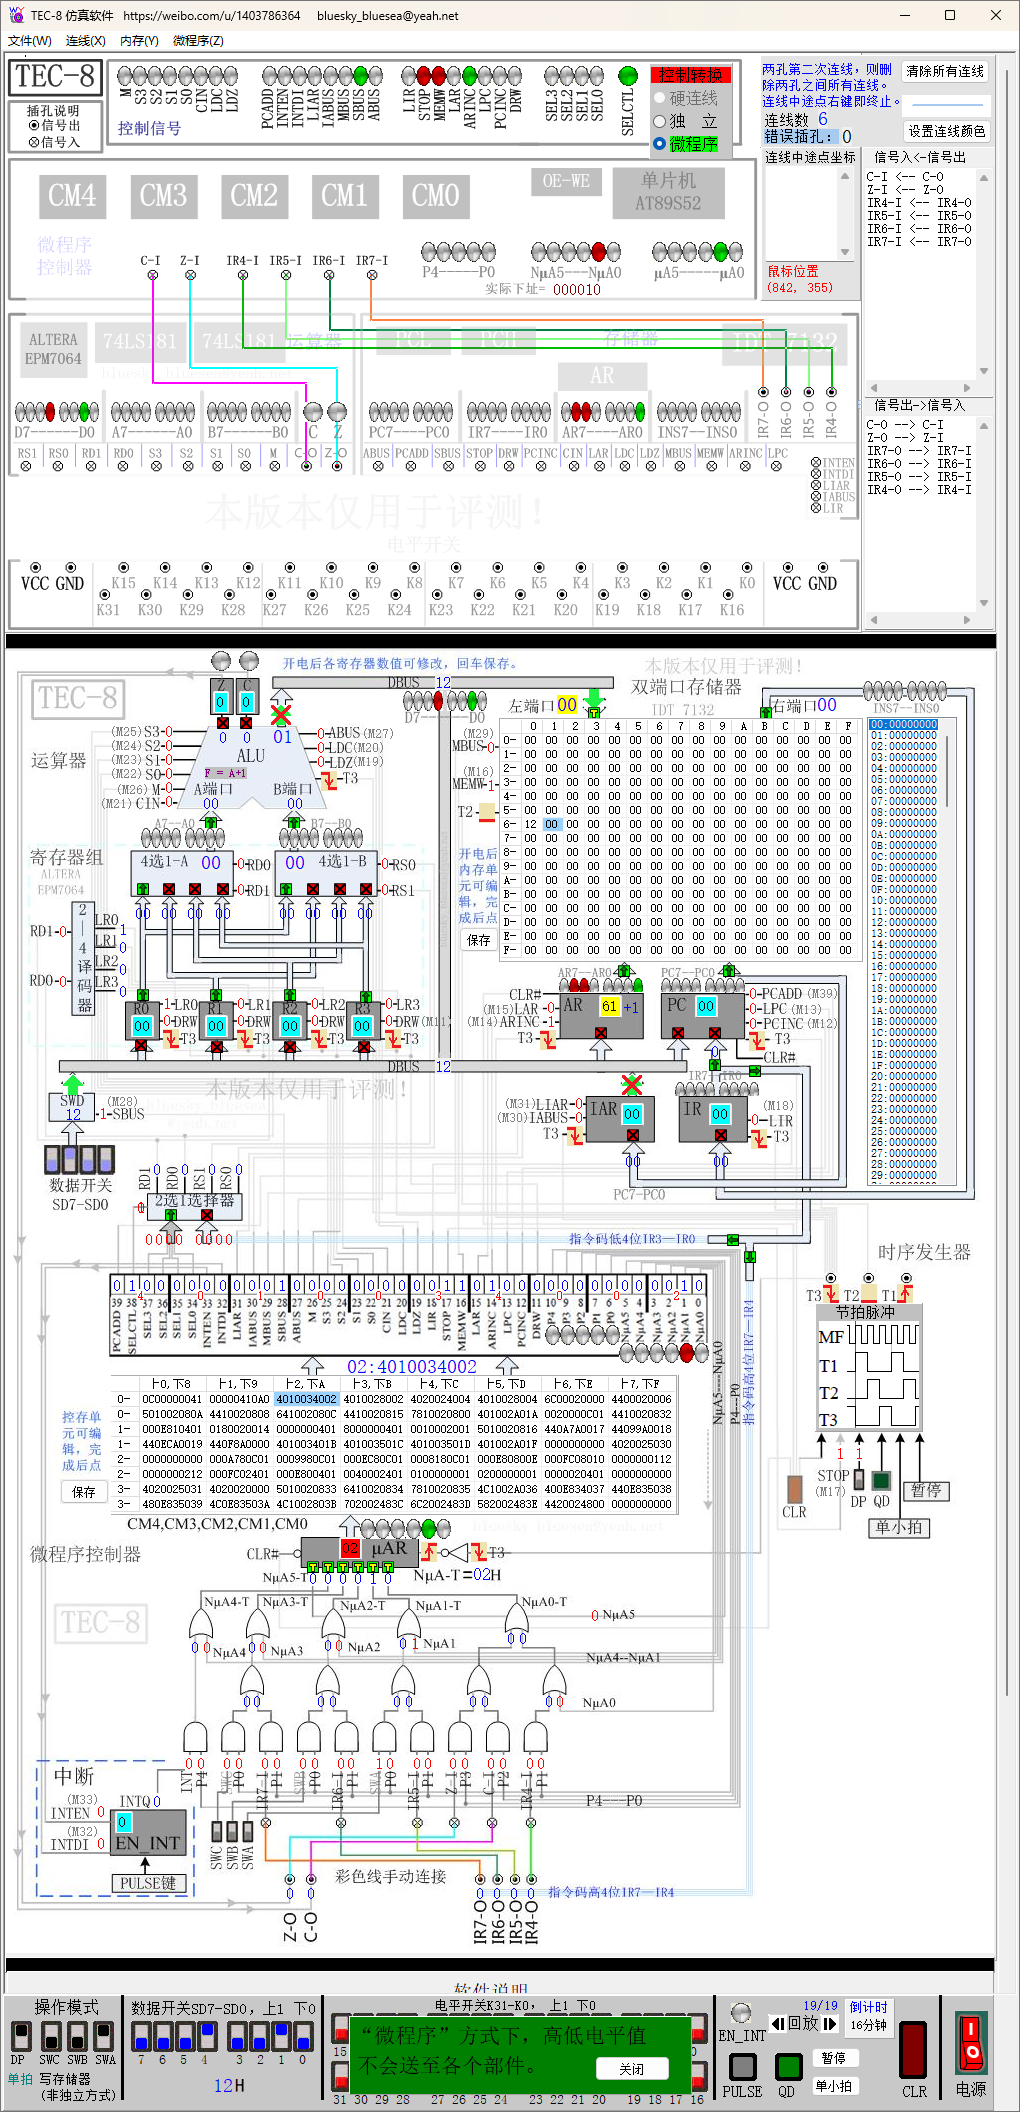
\includegraphics[width=0.3\textwidth]{screenshots/4.1.3.3.png}
    }
    \caption{写存储器}
    \label{fig: write memory}
\end{figure}

\begin{figure}[htbp]
    \centering
    \subfigure[]{
        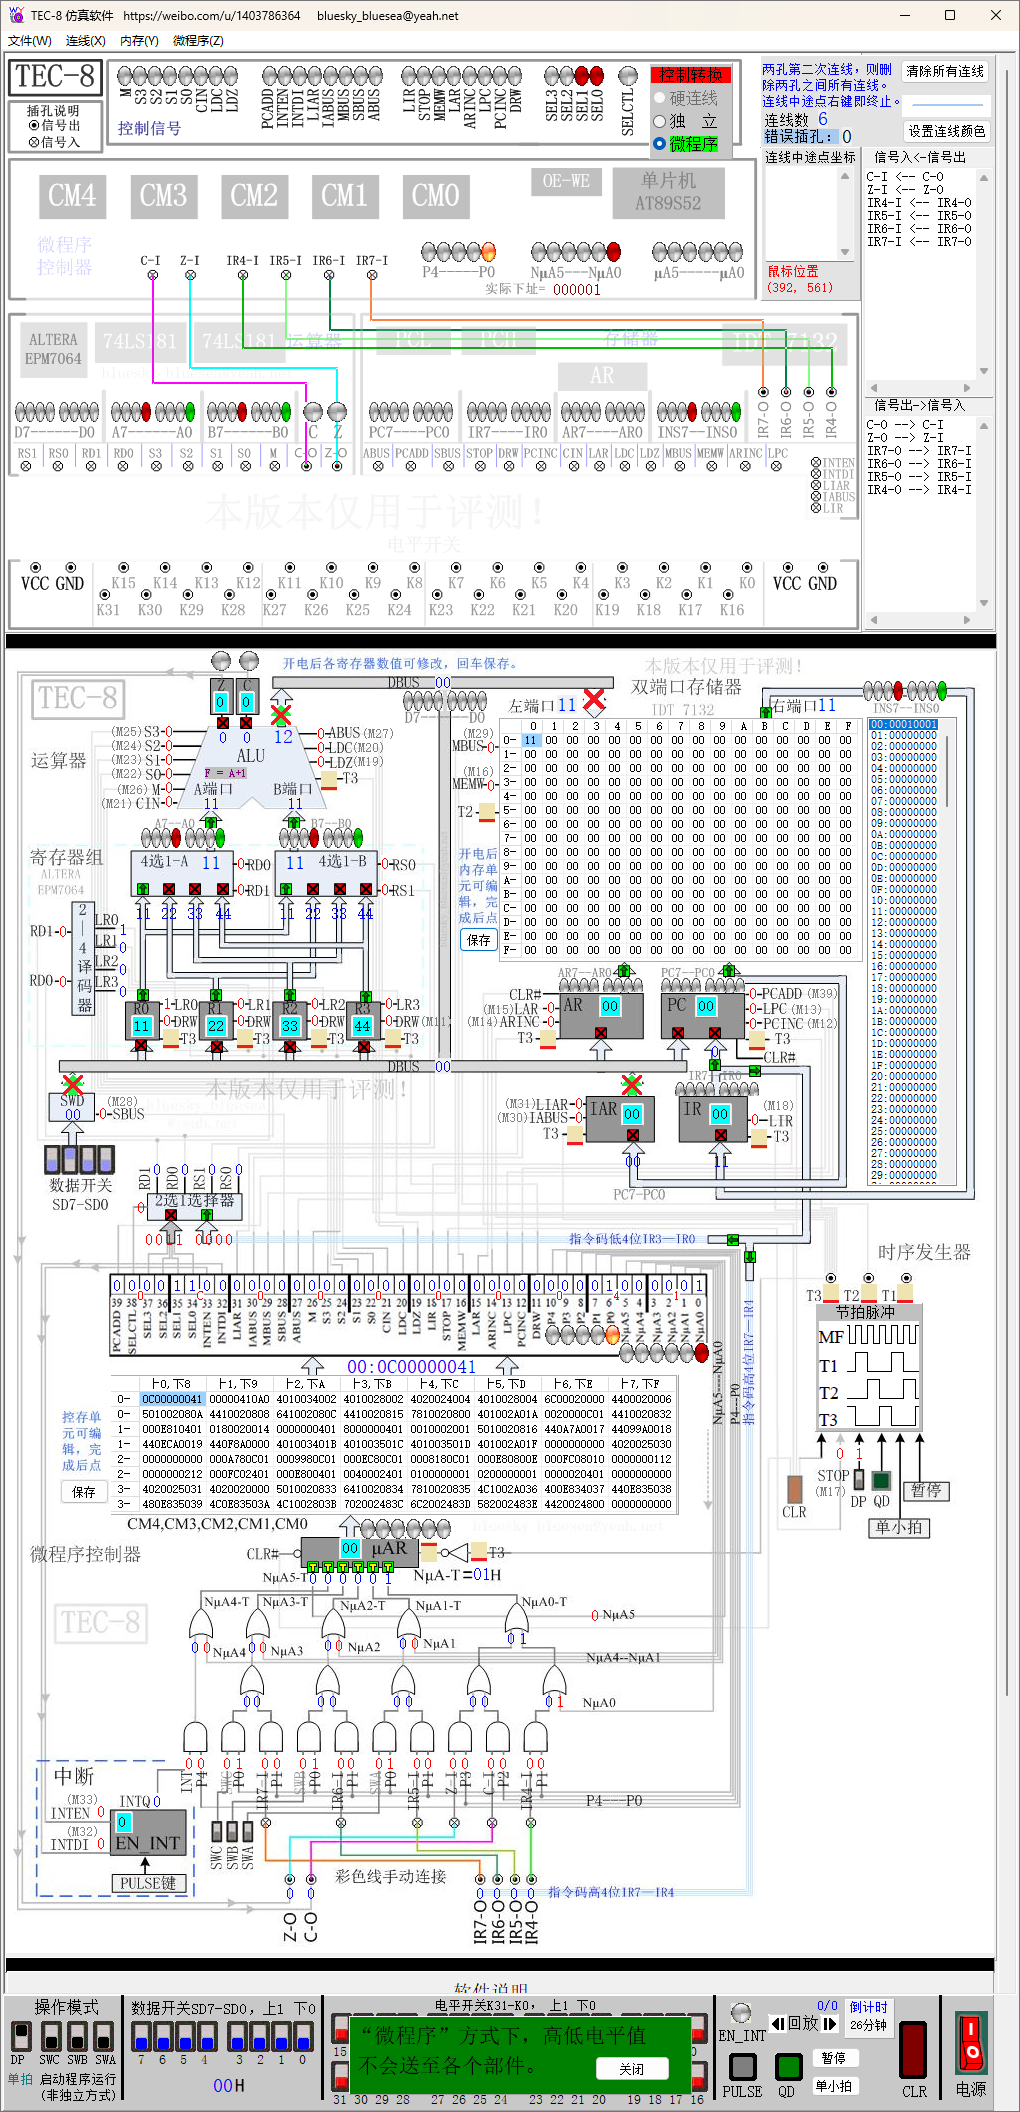
\includegraphics[width=0.3\textwidth]{screenshots/4.2.1.1.png}
    }
    \subfigure[]{
        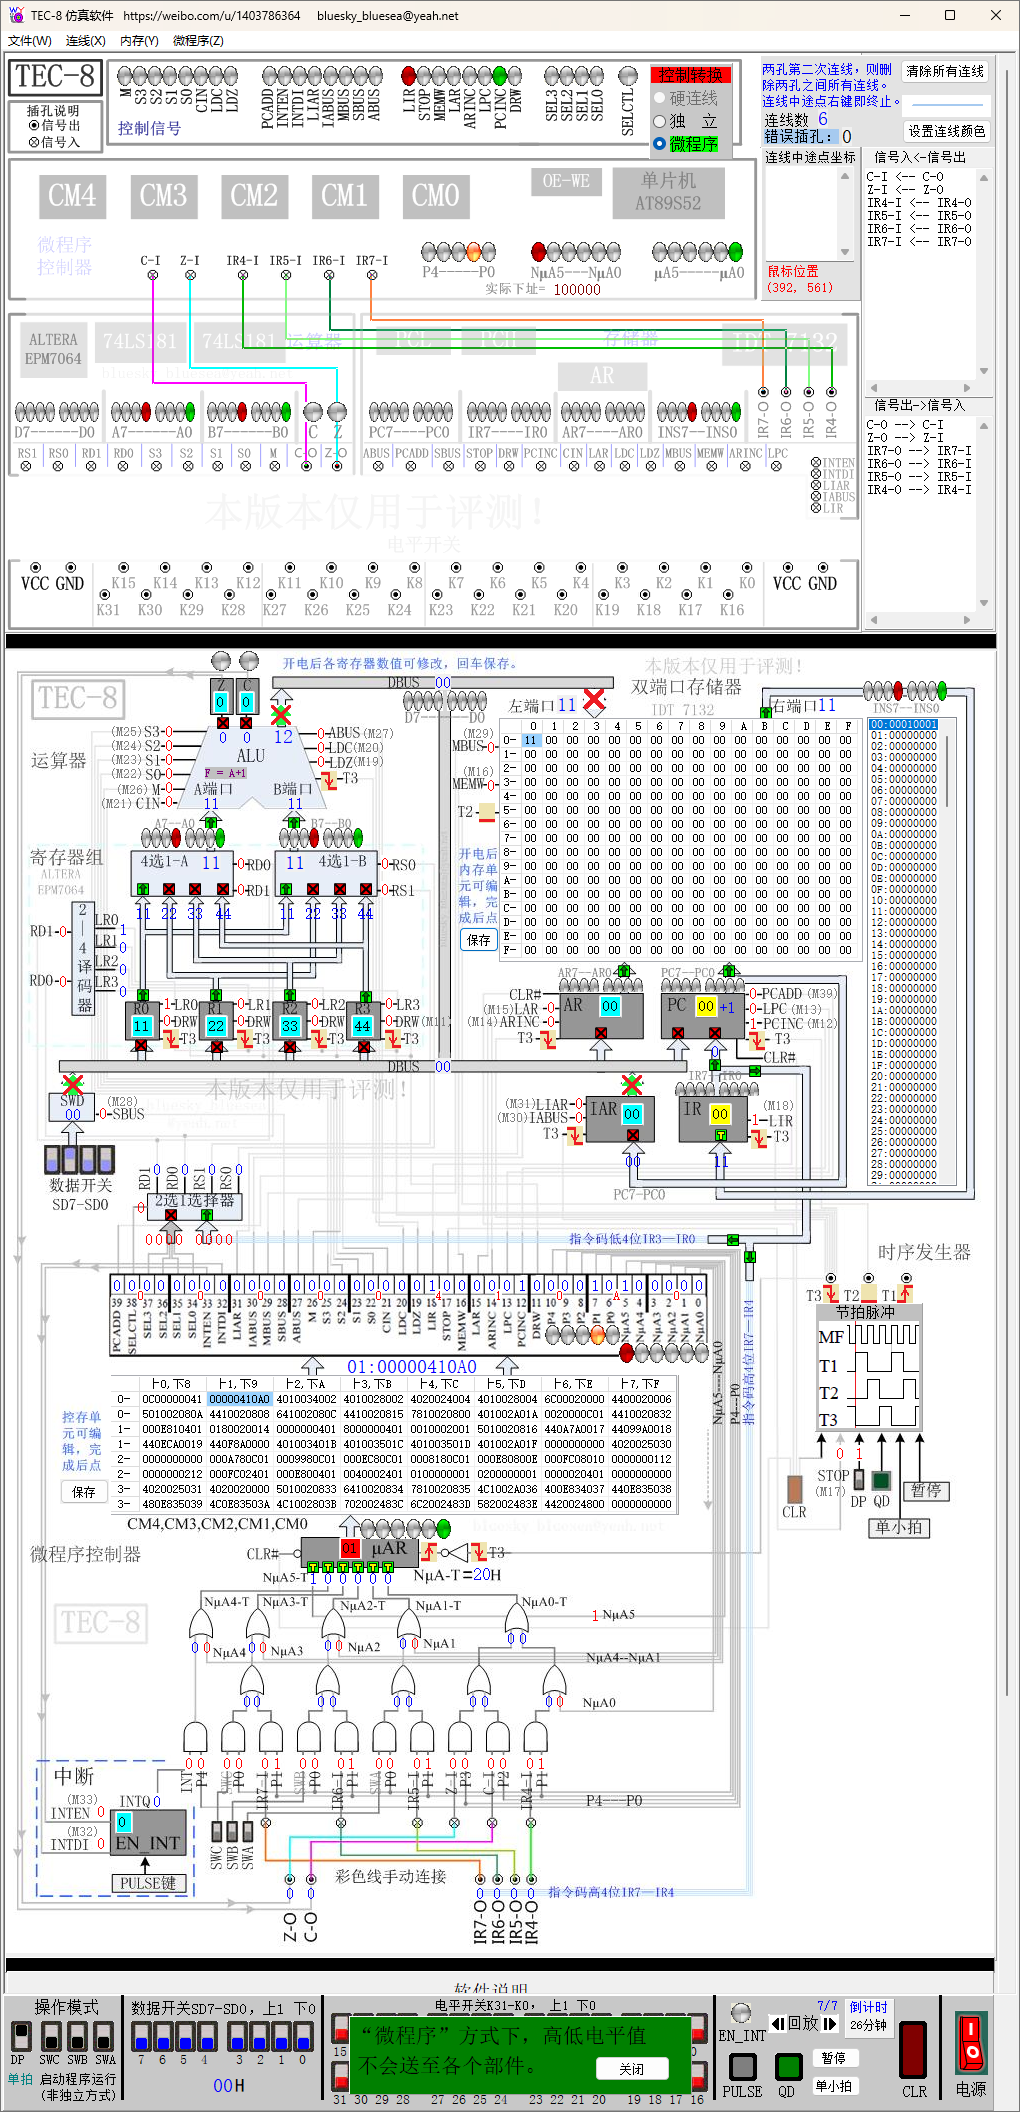
\includegraphics[width=0.3\textwidth]{screenshots/4.2.1.2.png}
    }
    \\
    \subfigure[]{
        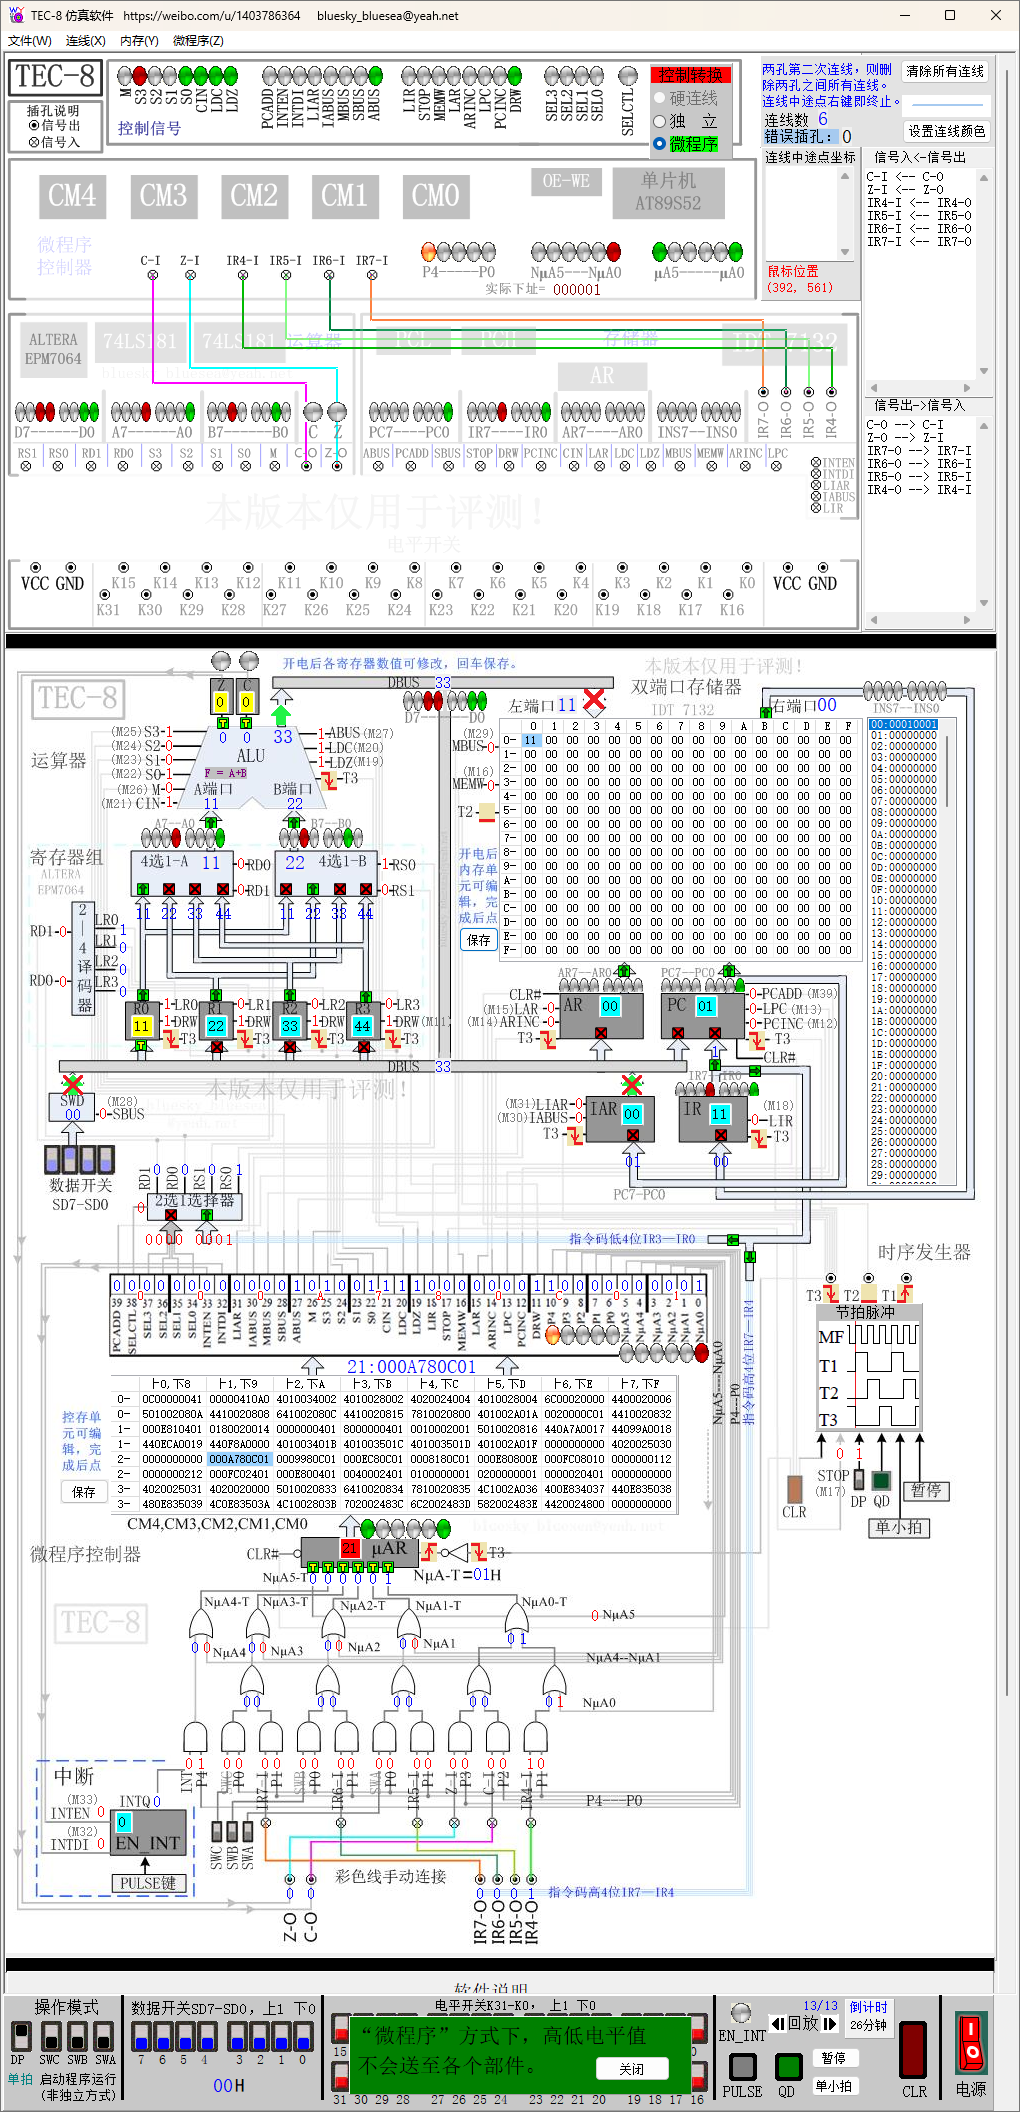
\includegraphics[width=0.3\textwidth]{screenshots/4.2.1.3.png}
    }
    \subfigure[]{
        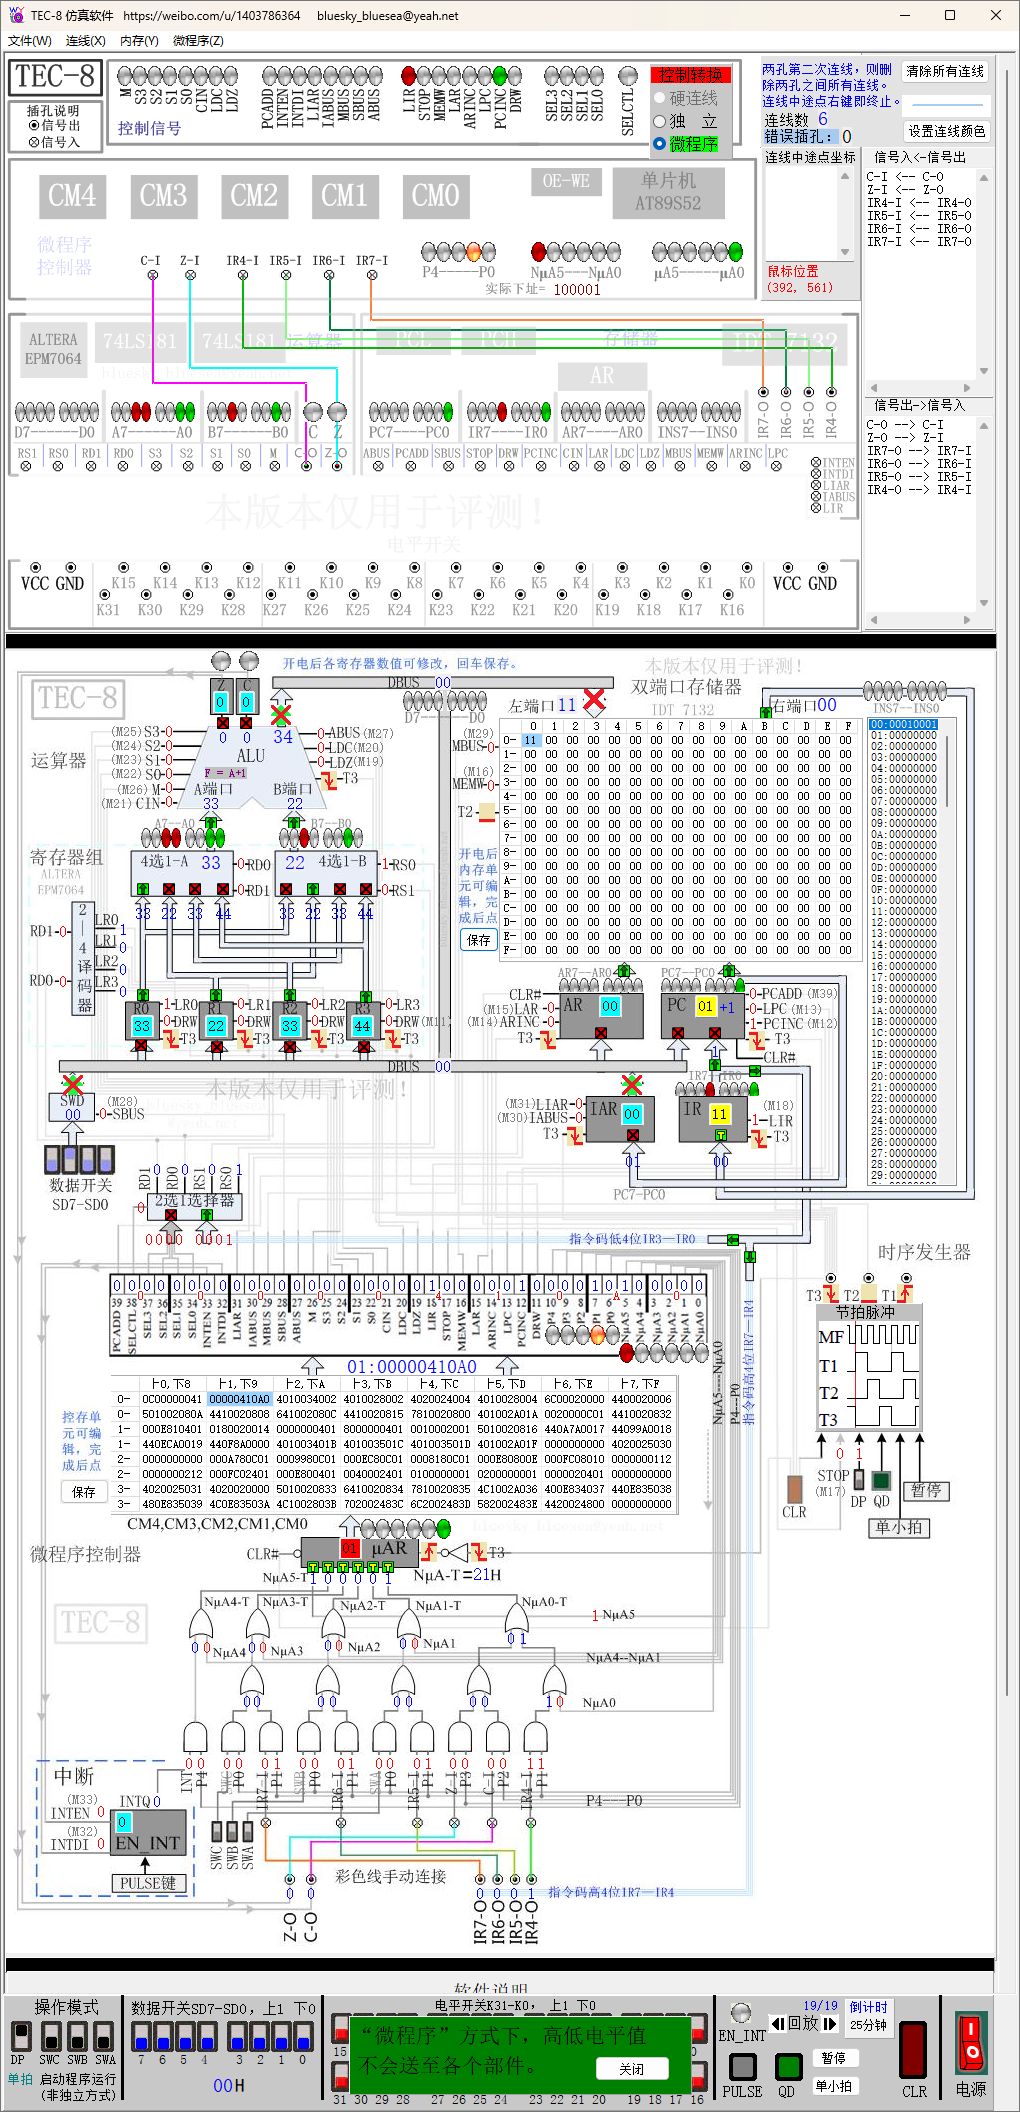
\includegraphics[width=0.3\textwidth]{screenshots/4.2.1.4.png}
    }
    \caption{加法}
    \label{fig: add}
\end{figure}

\begin{figure}[htbp]
    \centering
    \subfigure[]{
        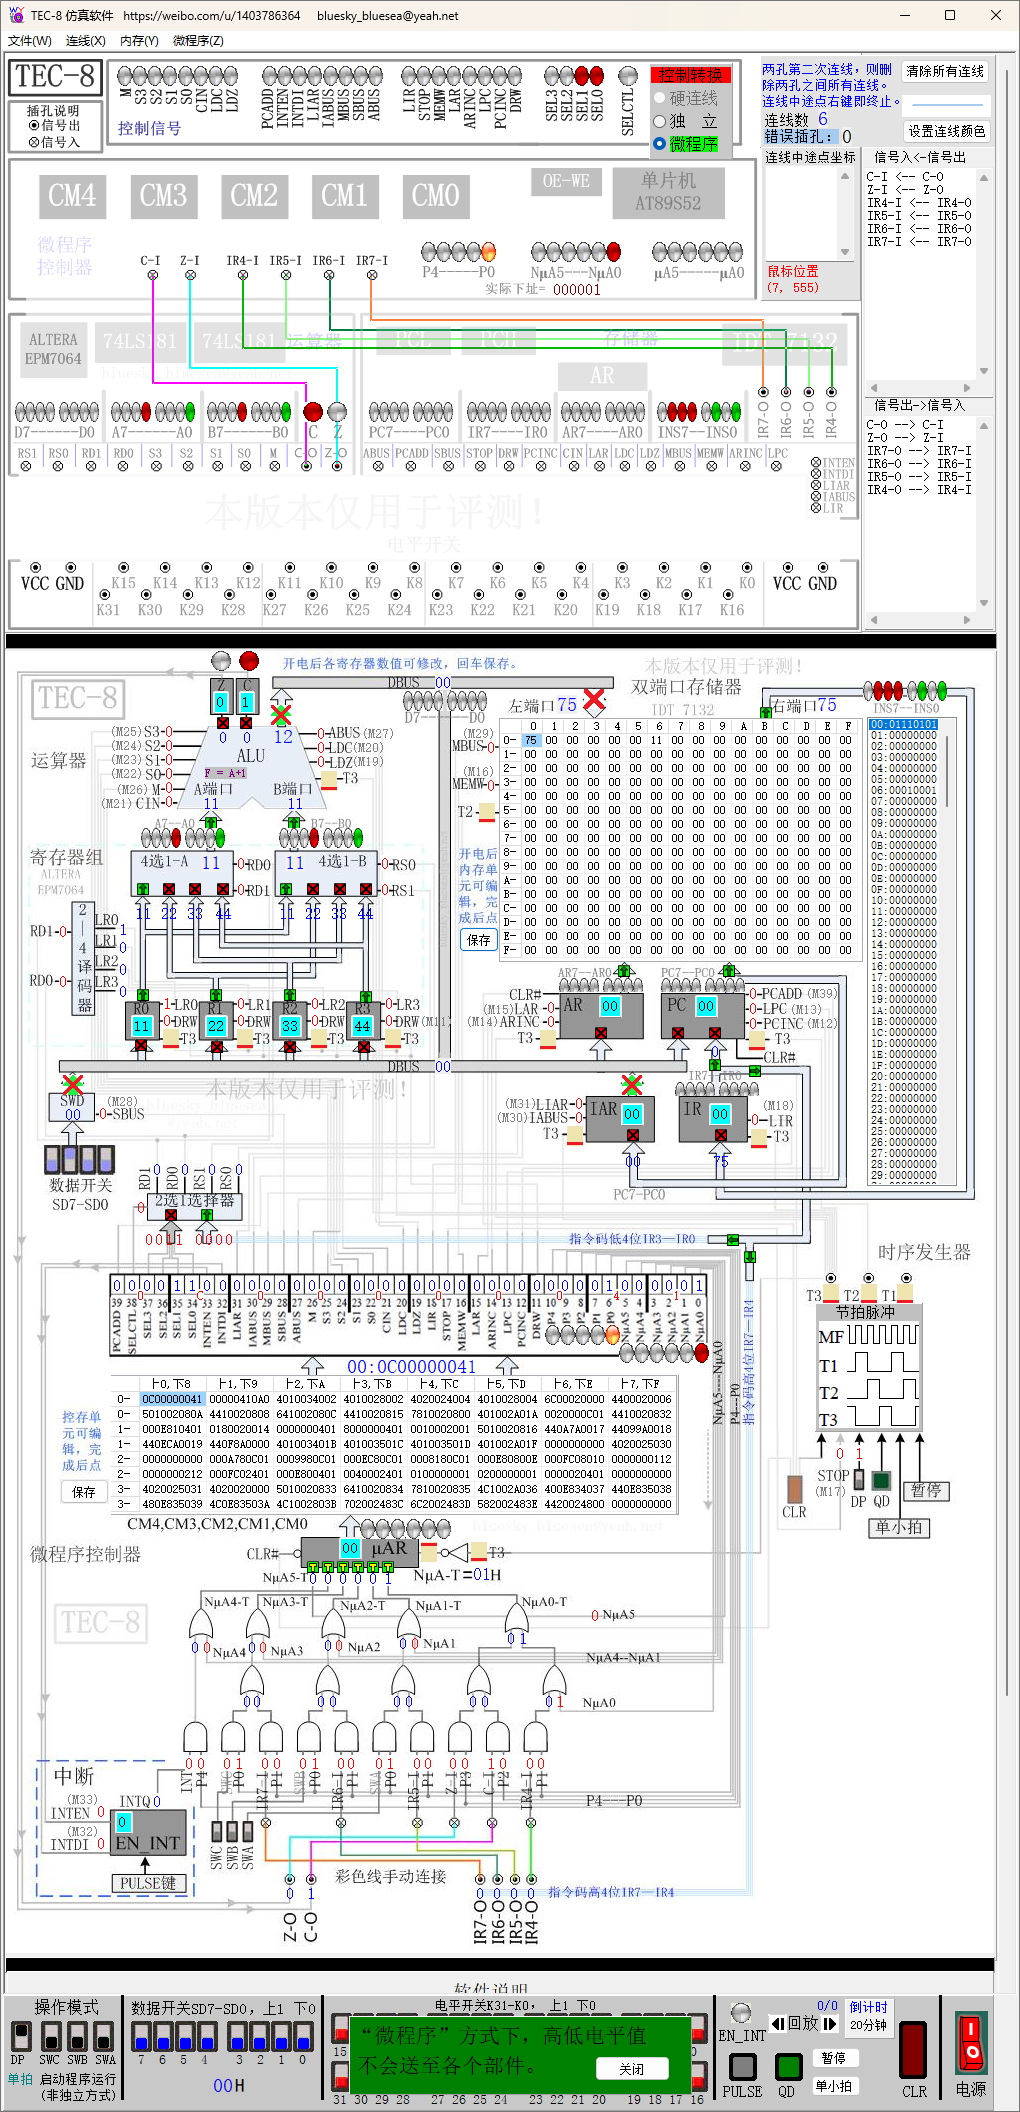
\includegraphics[width=0.3\textwidth]{screenshots/4.2.2.1.png}
    }
    \subfigure[]{
        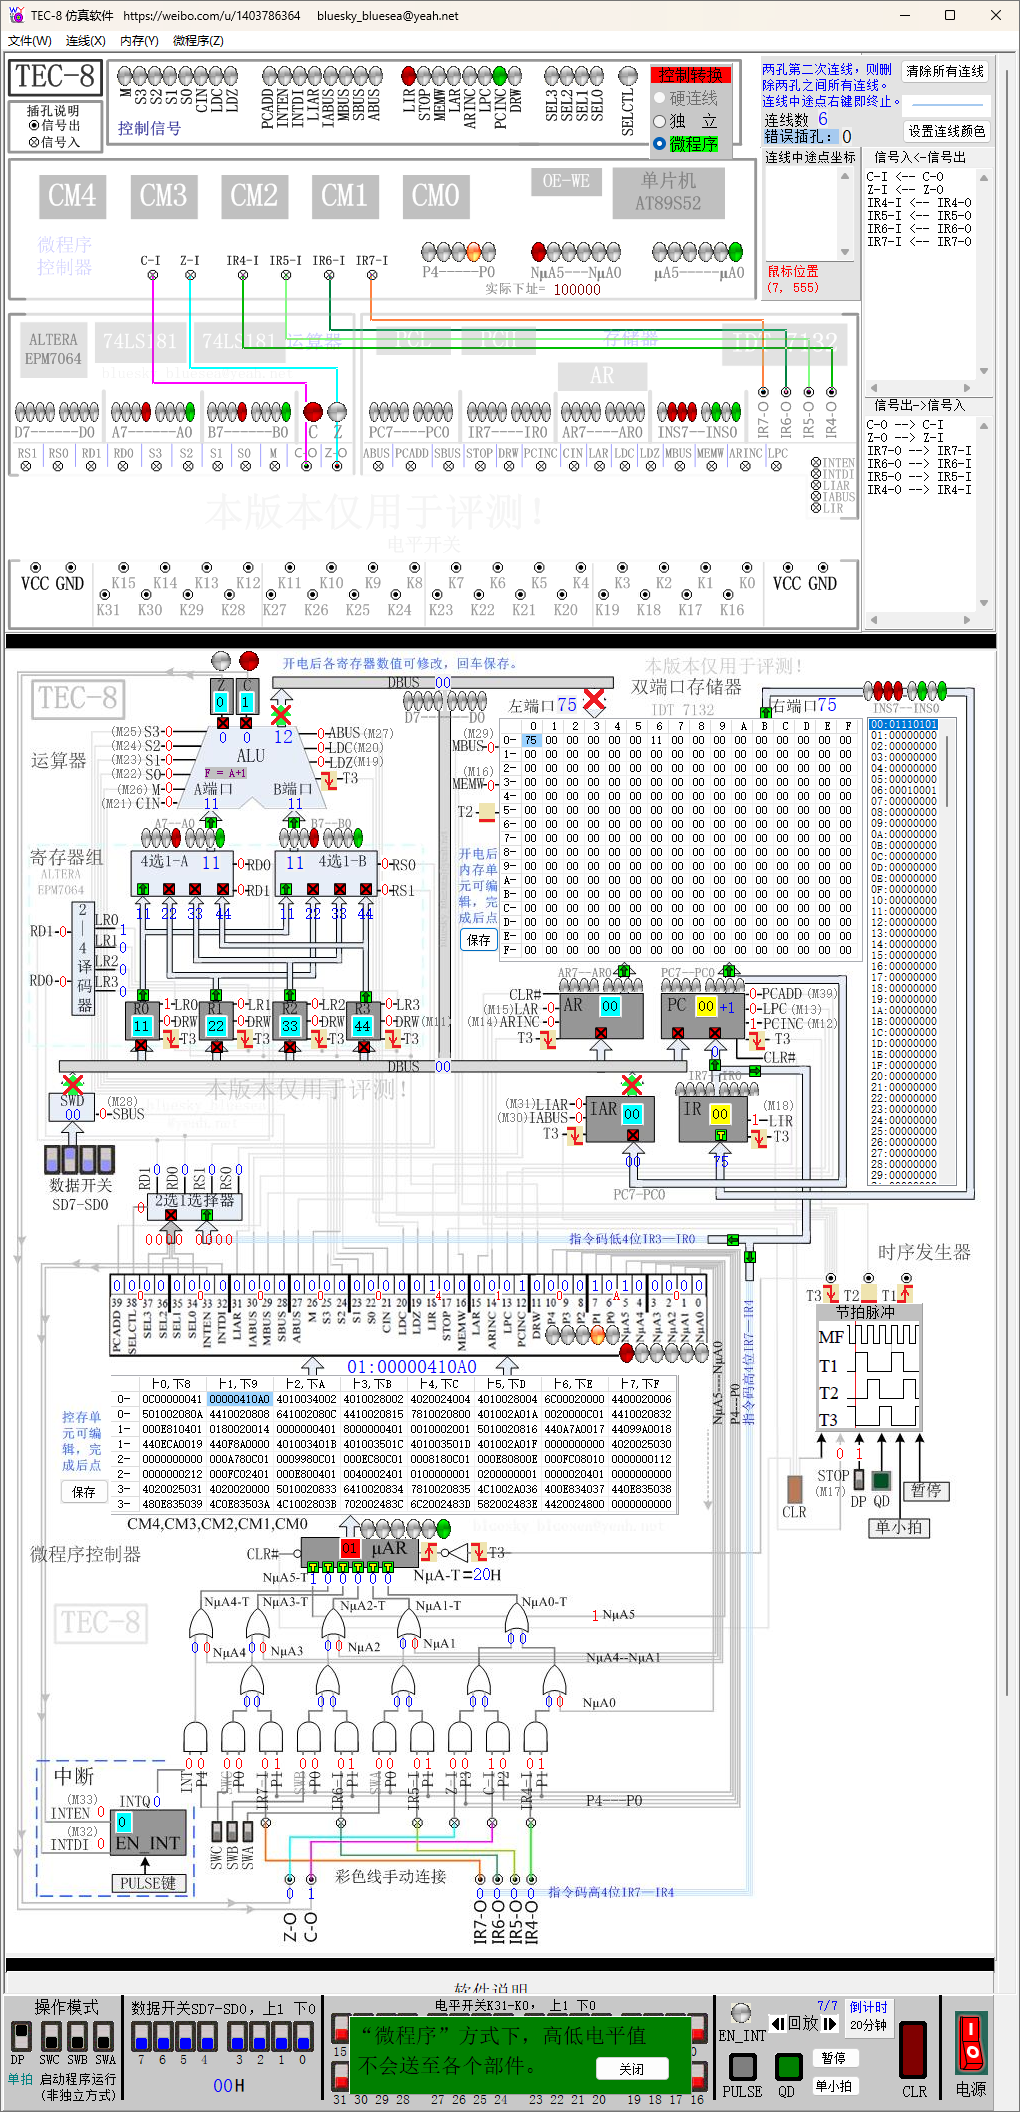
\includegraphics[width=0.3\textwidth]{screenshots/4.2.2.2.png}
    }
    \subfigure[]{
        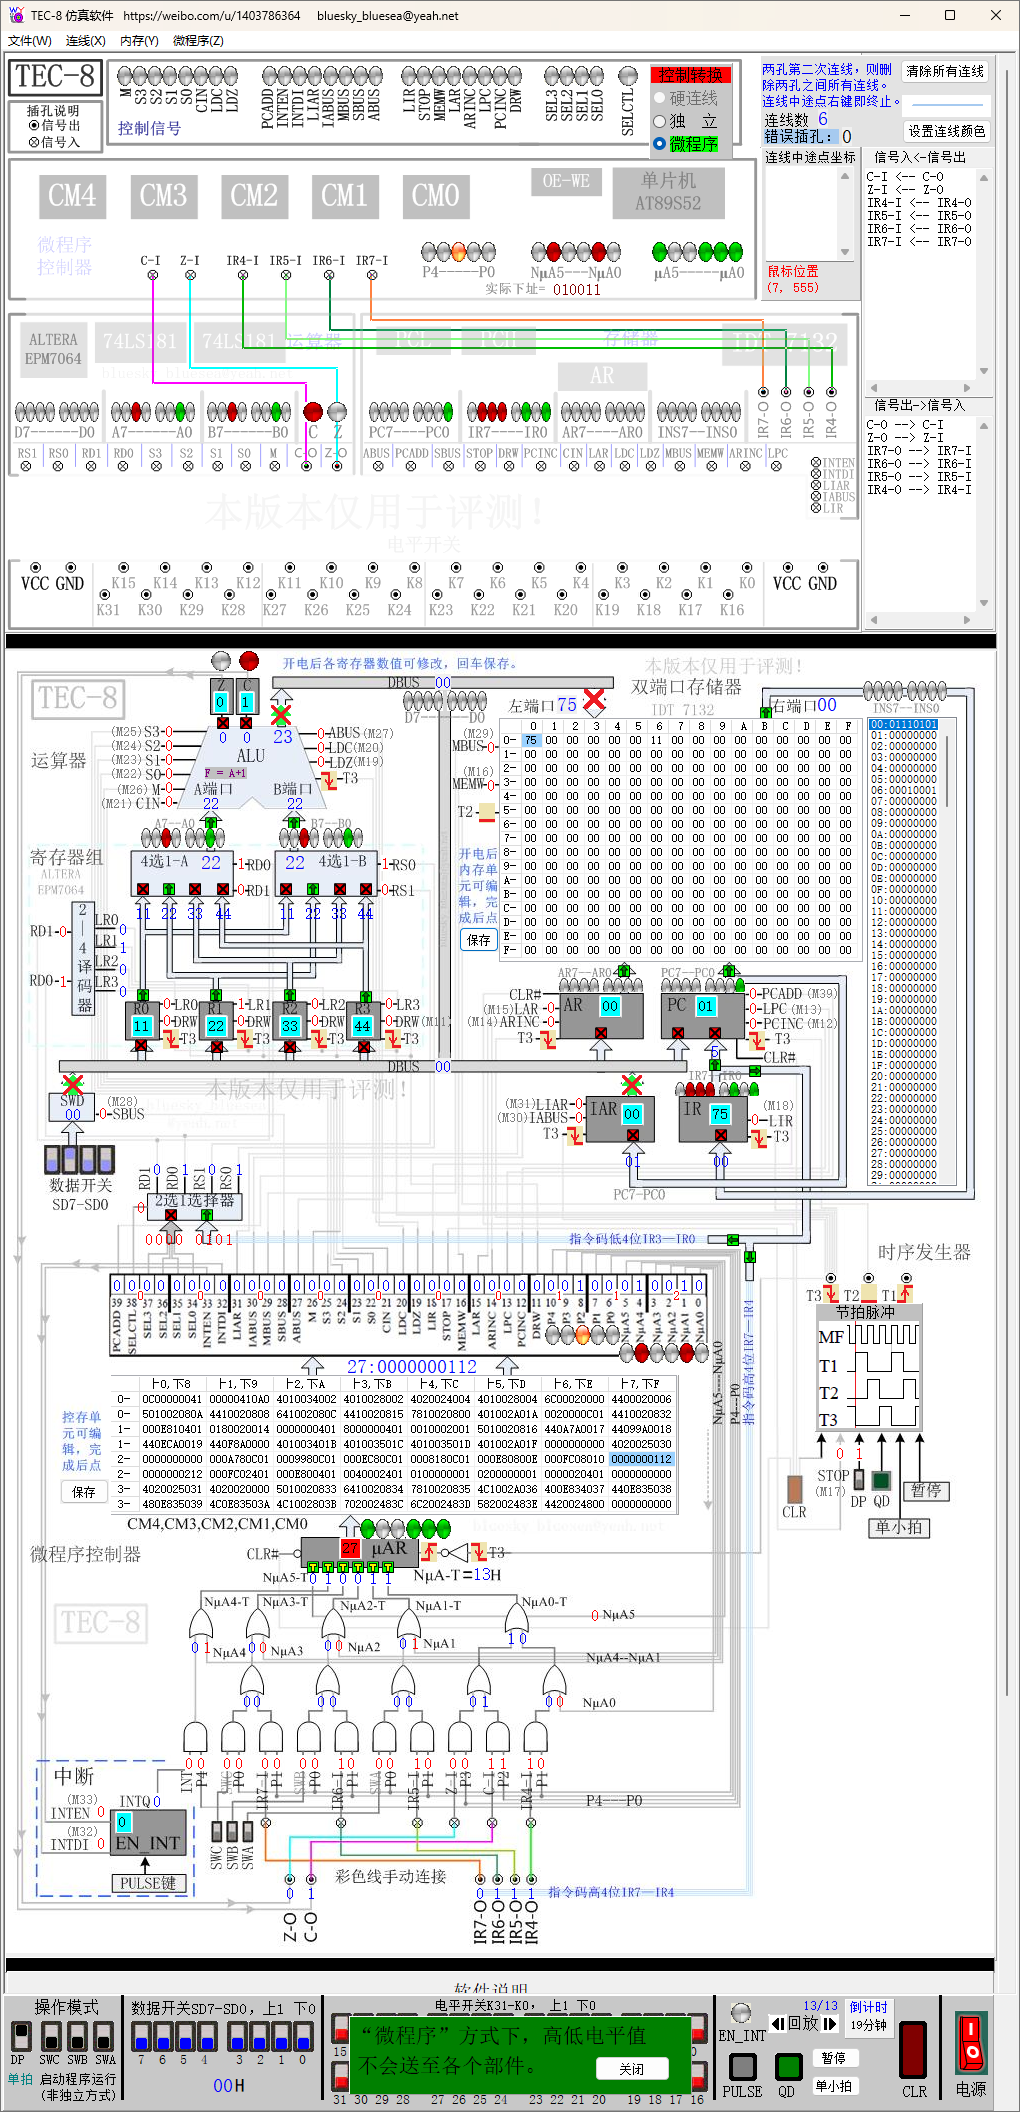
\includegraphics[width=0.3\textwidth]{screenshots/4.2.2.3.png}
    }
    \\
    \subfigure[]{
        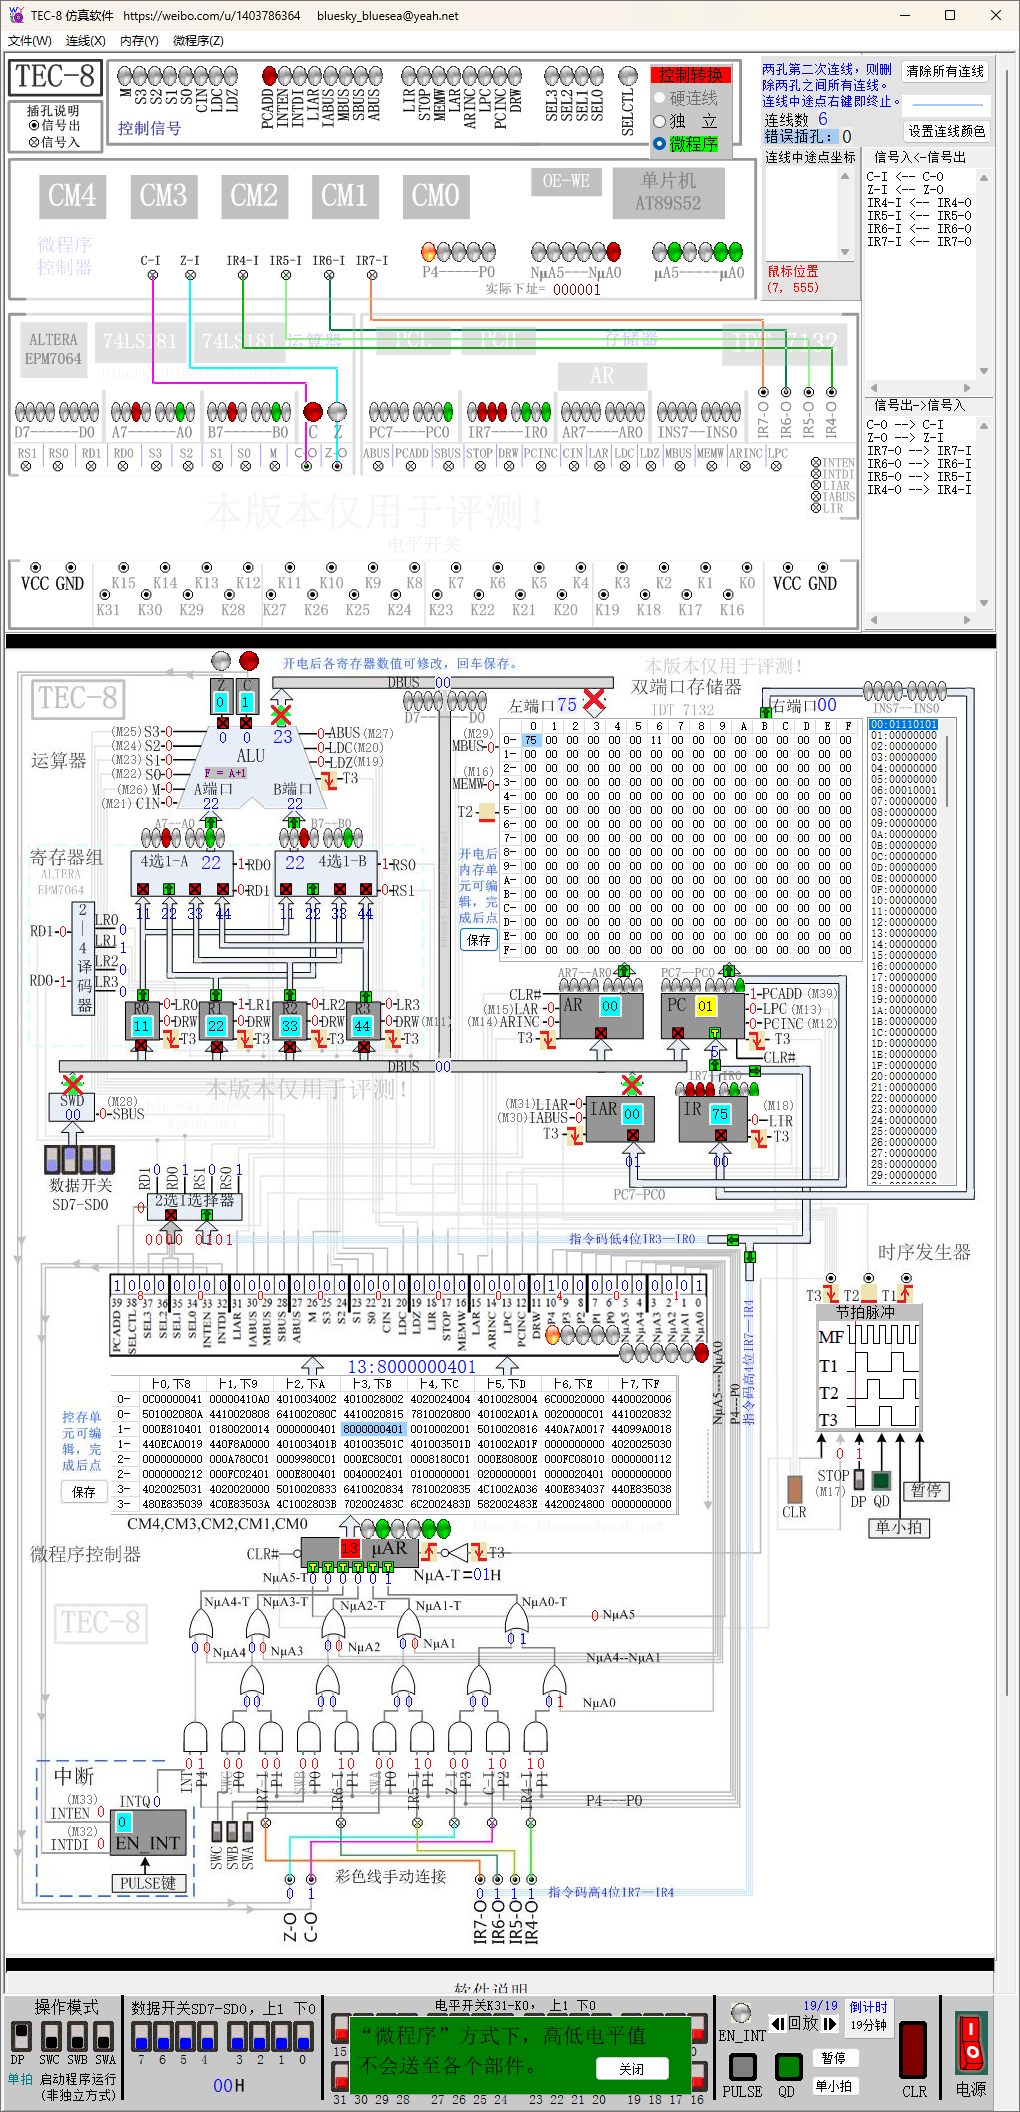
\includegraphics[width=0.3\textwidth]{screenshots/4.2.2.4.png}
    }
    \subfigure[]{
        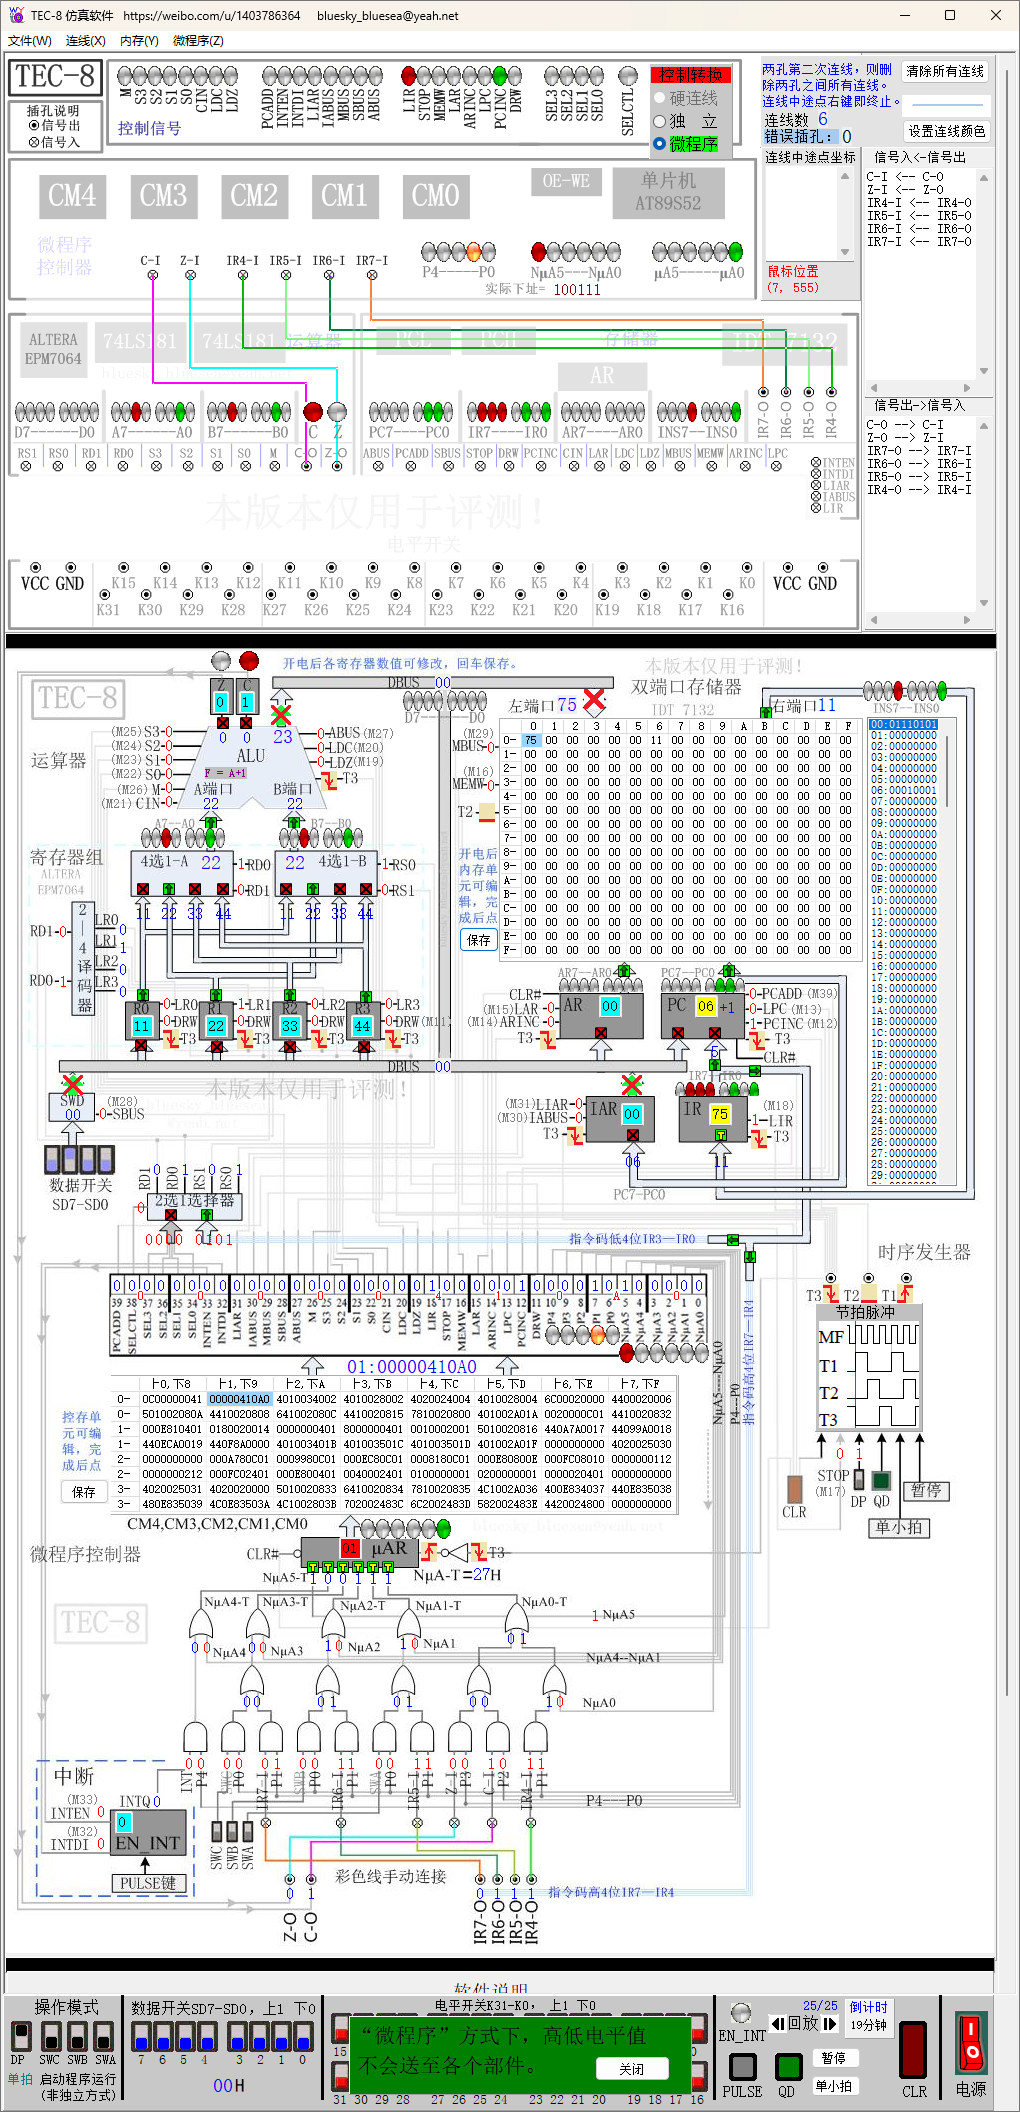
\includegraphics[width=0.3\textwidth]{screenshots/4.2.2.5.png}
    }
    \caption{C条件转移}
    \label{fig: jmp}
\end{figure}

\begin{figure}[htbp]
    \centering
    \subfigure[]{
        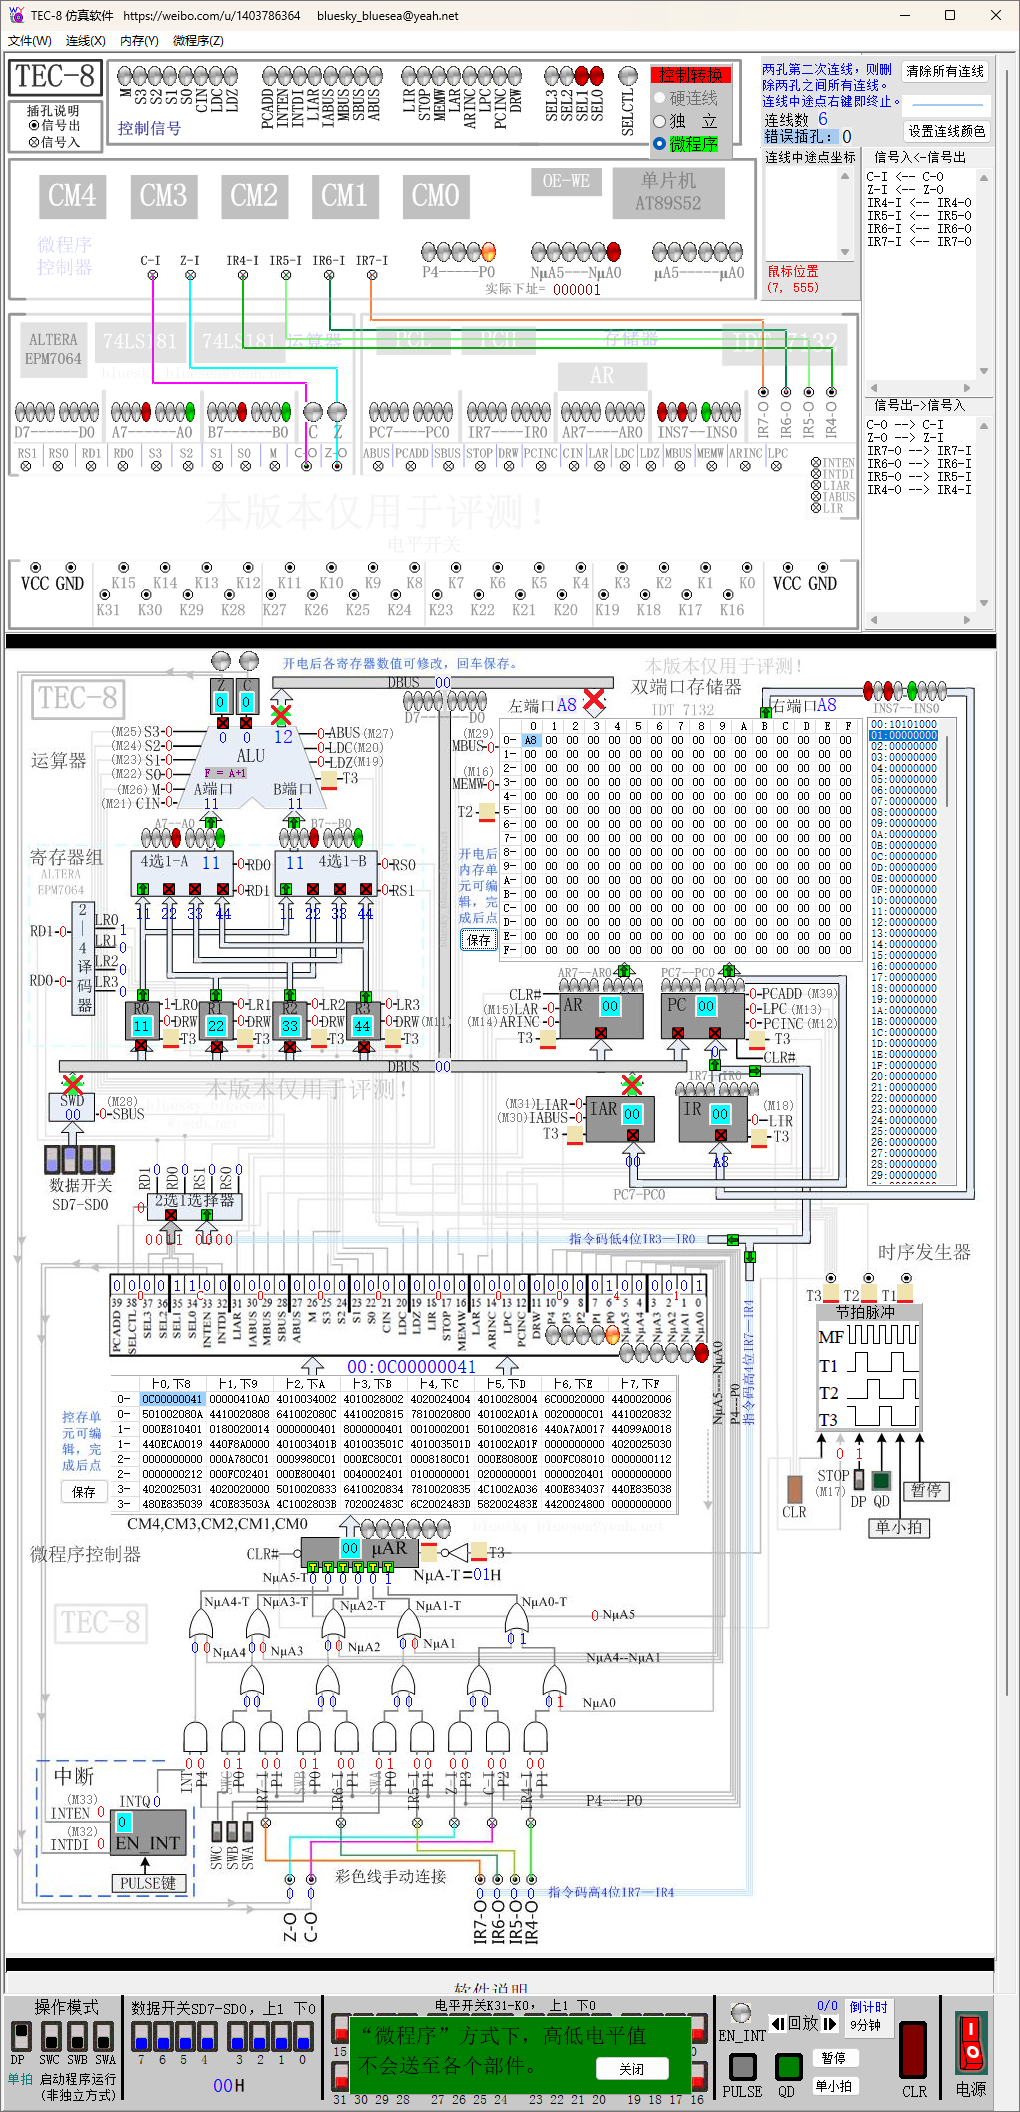
\includegraphics[width=0.3\textwidth]{screenshots/4.2.4.1.png}
    }
    \subfigure[]{
        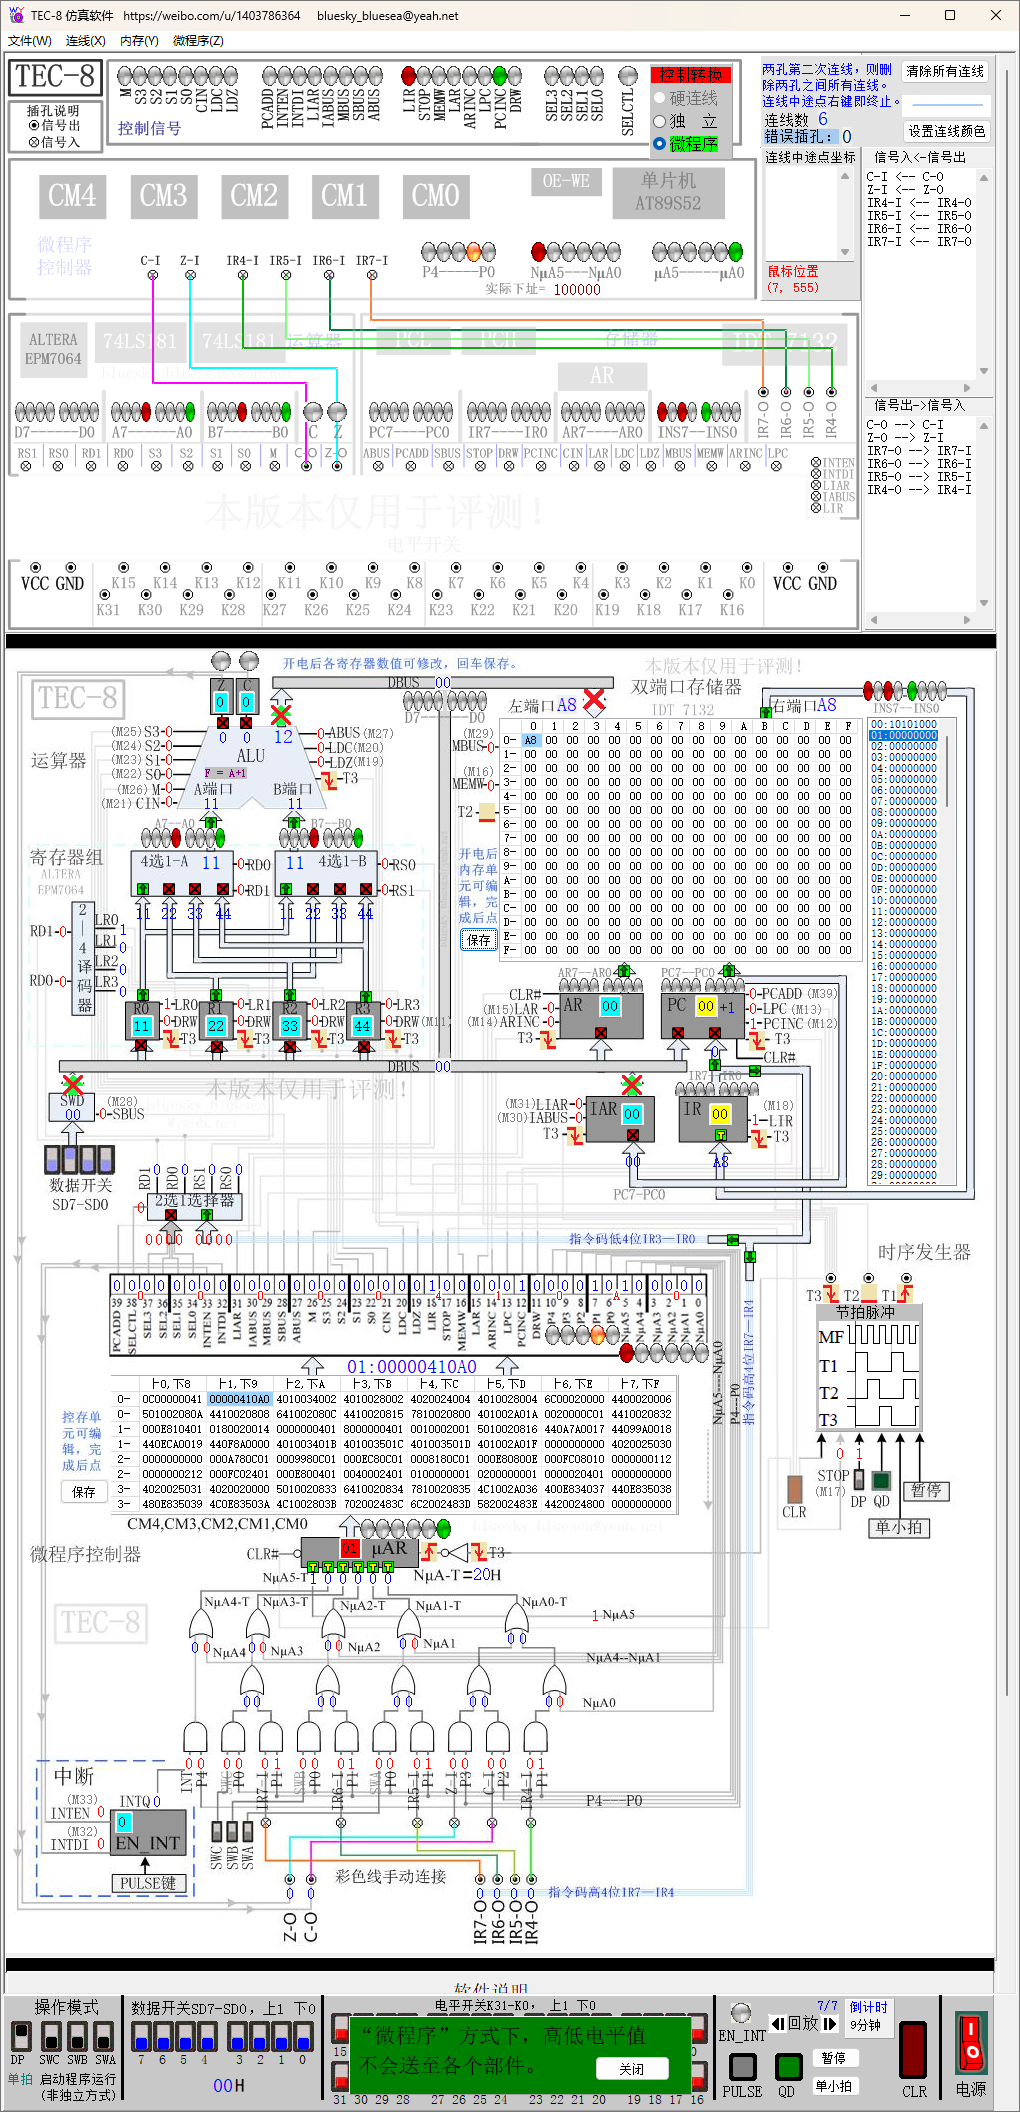
\includegraphics[width=0.3\textwidth]{screenshots/4.2.4.2.png}
    }
    \\
    \subfigure[]{
        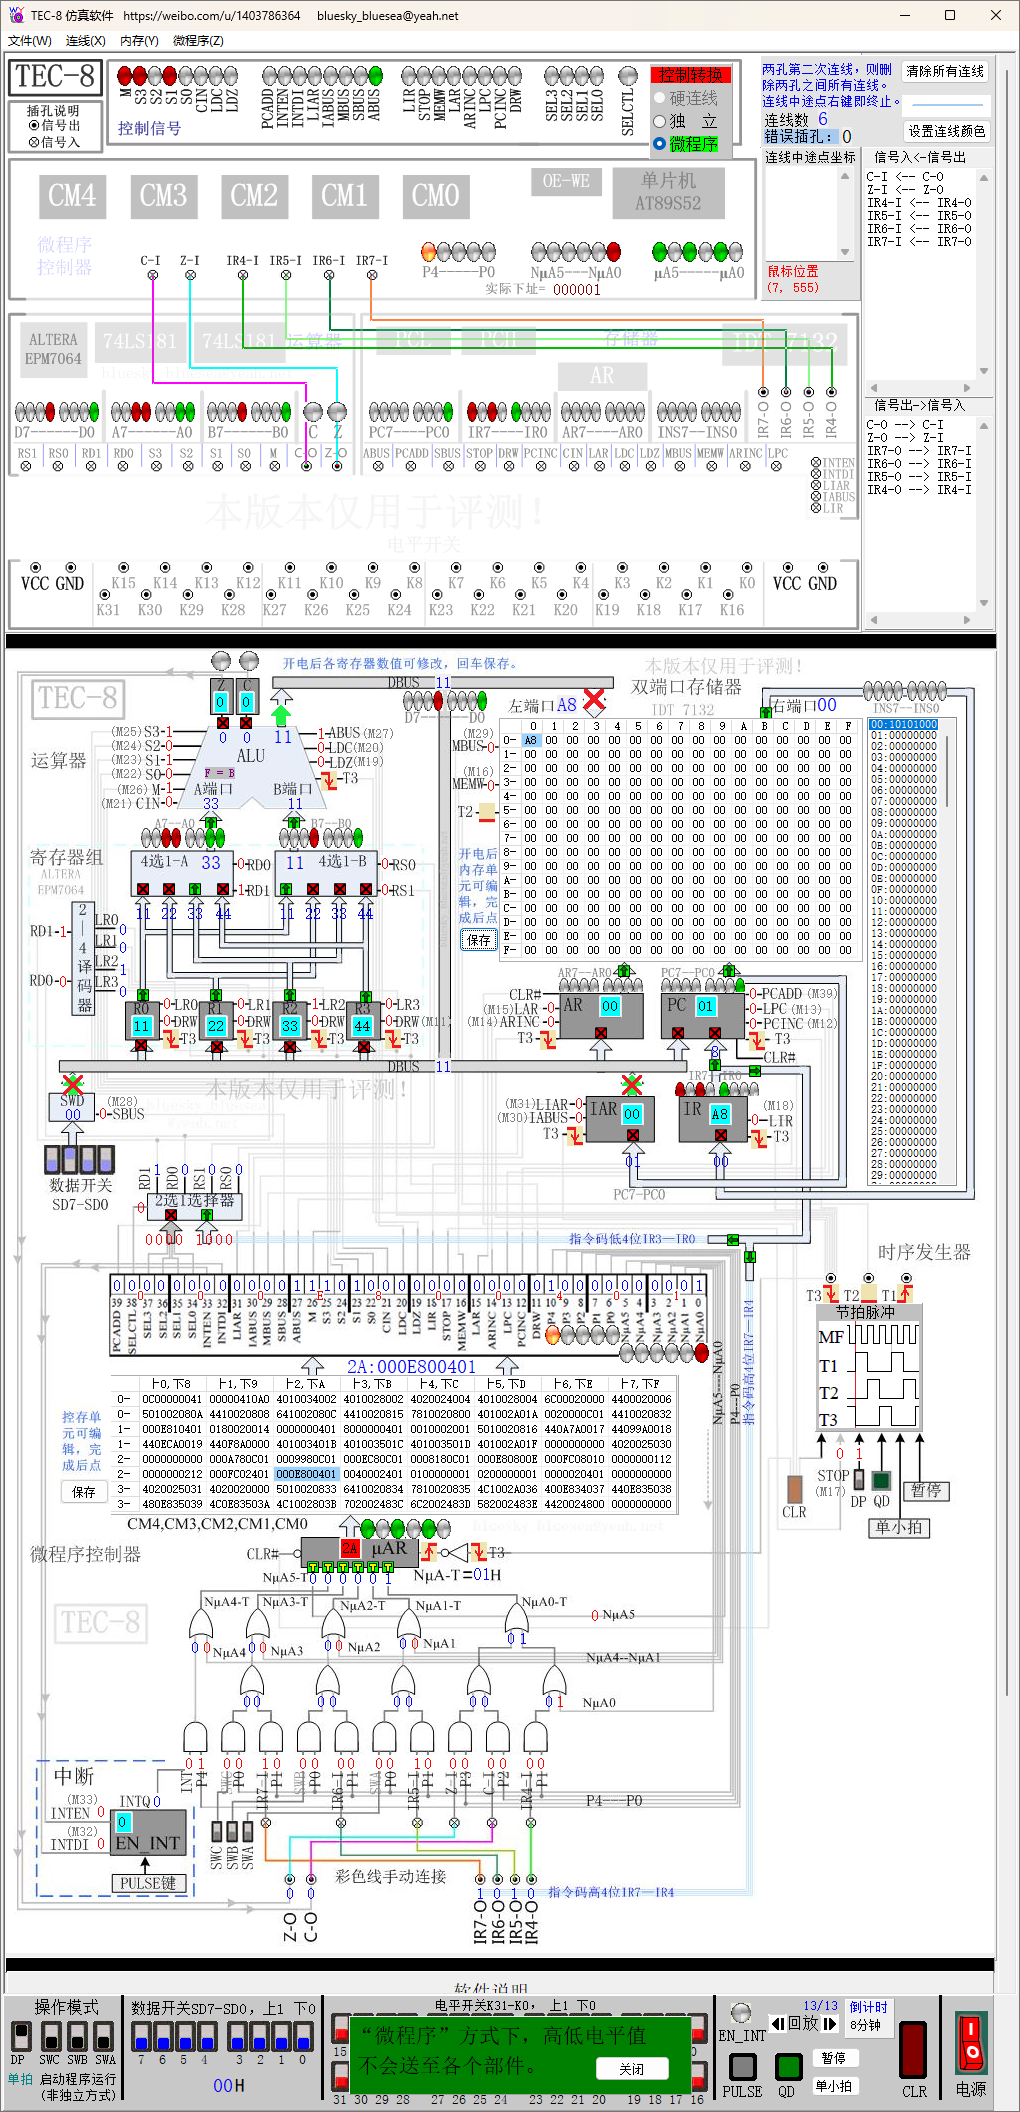
\includegraphics[width=0.3\textwidth]{screenshots/4.2.4.3.png}
    }
    \subfigure[]{
        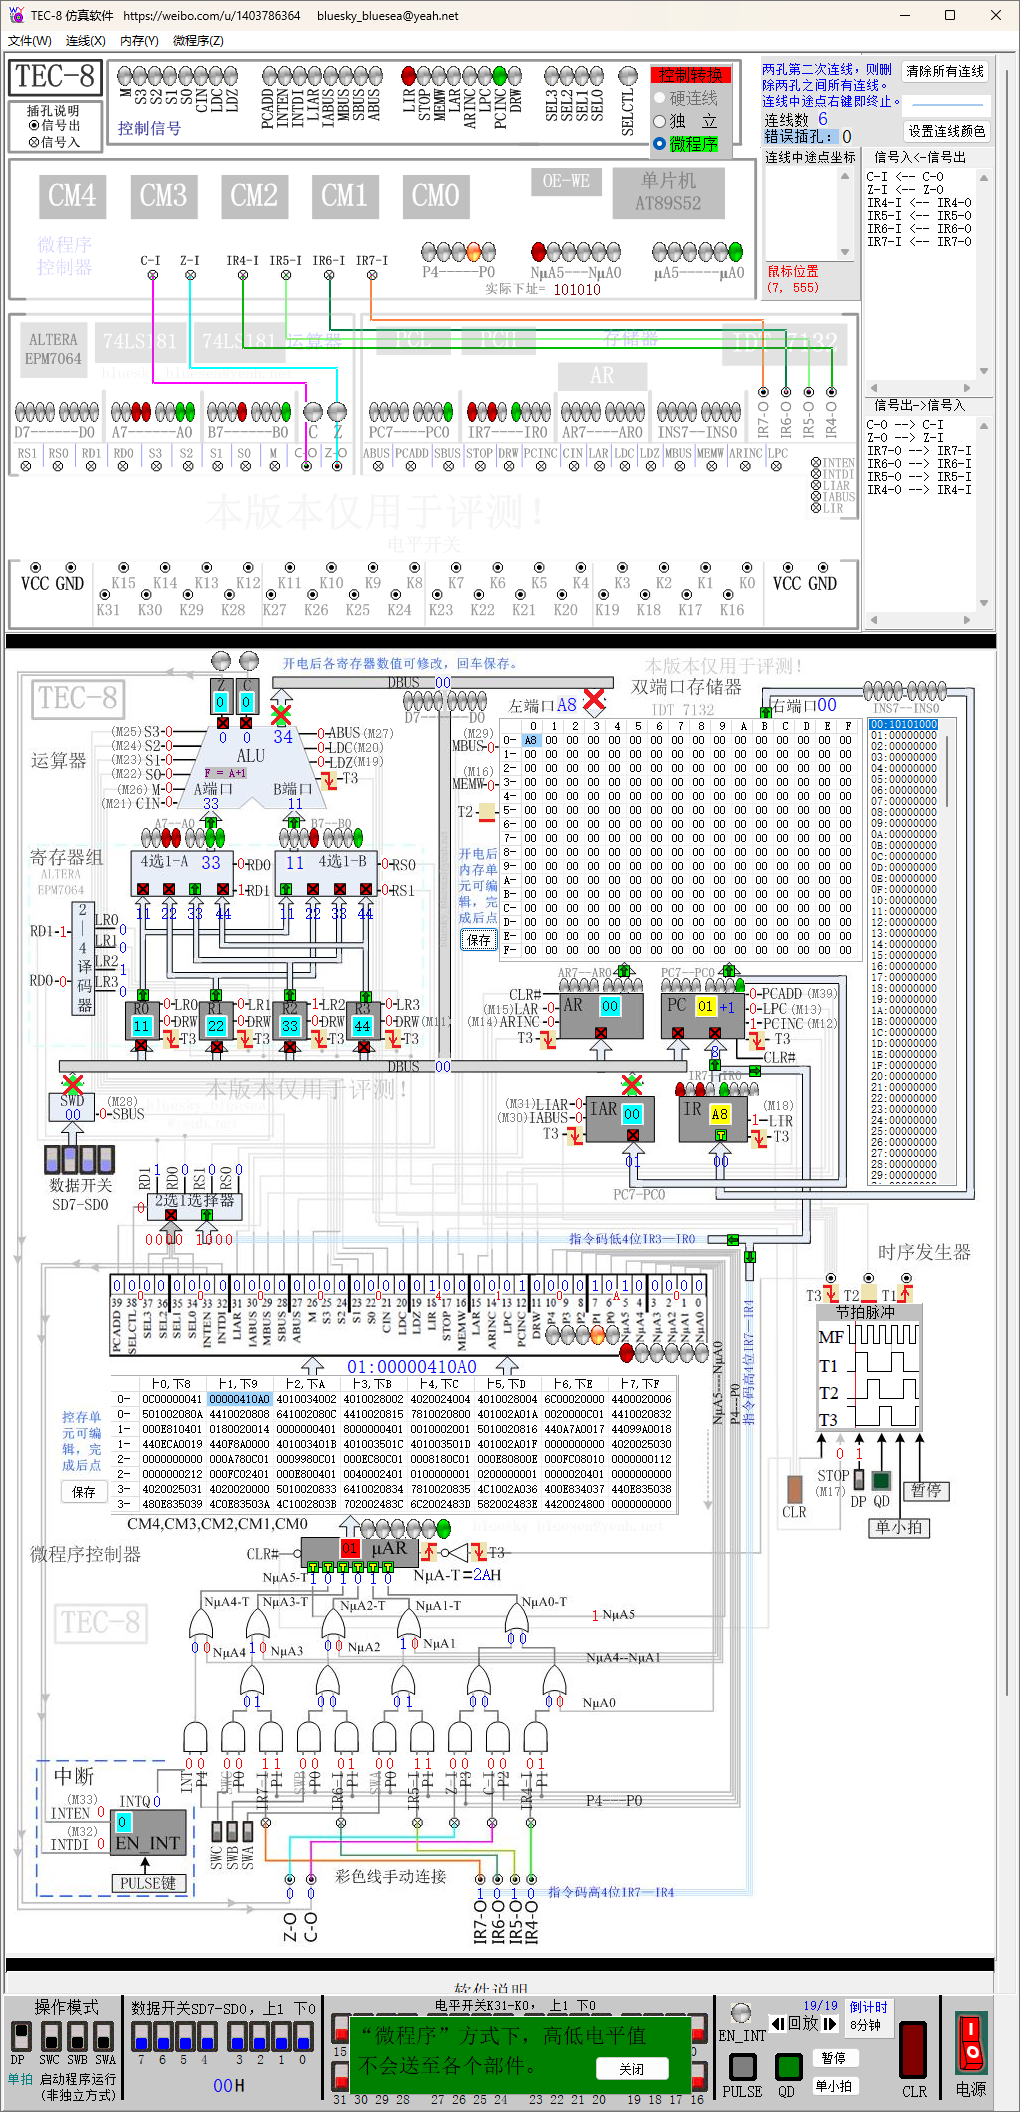
\includegraphics[width=0.3\textwidth]{screenshots/4.2.4.4.png}
    }
    \caption{输出}
    \label{fig: out}
\end{figure}

\begin{figure}[htbp]
    \centering
    \subfigure[]{
        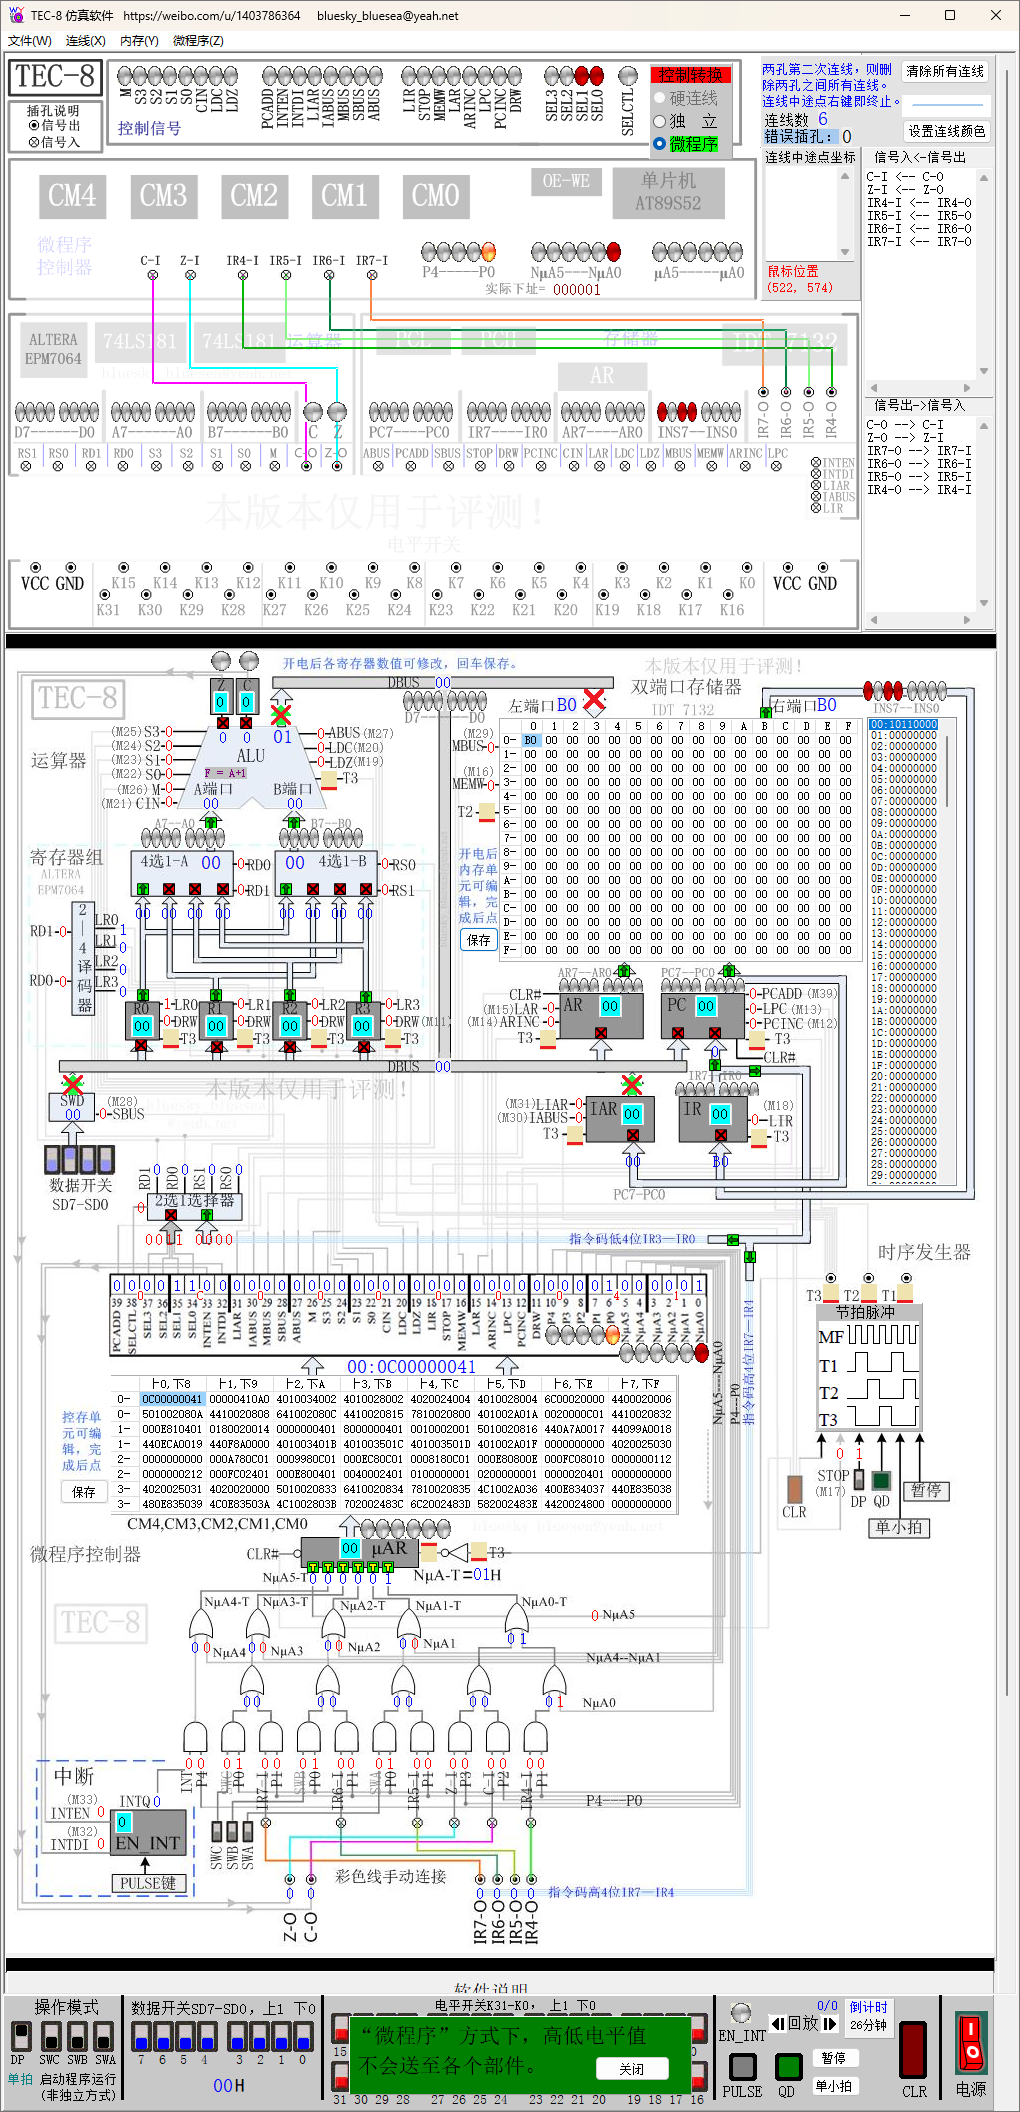
\includegraphics[width=0.3\textwidth]{screenshots/4.2.5.1.png}
    }
    \subfigure[]{
        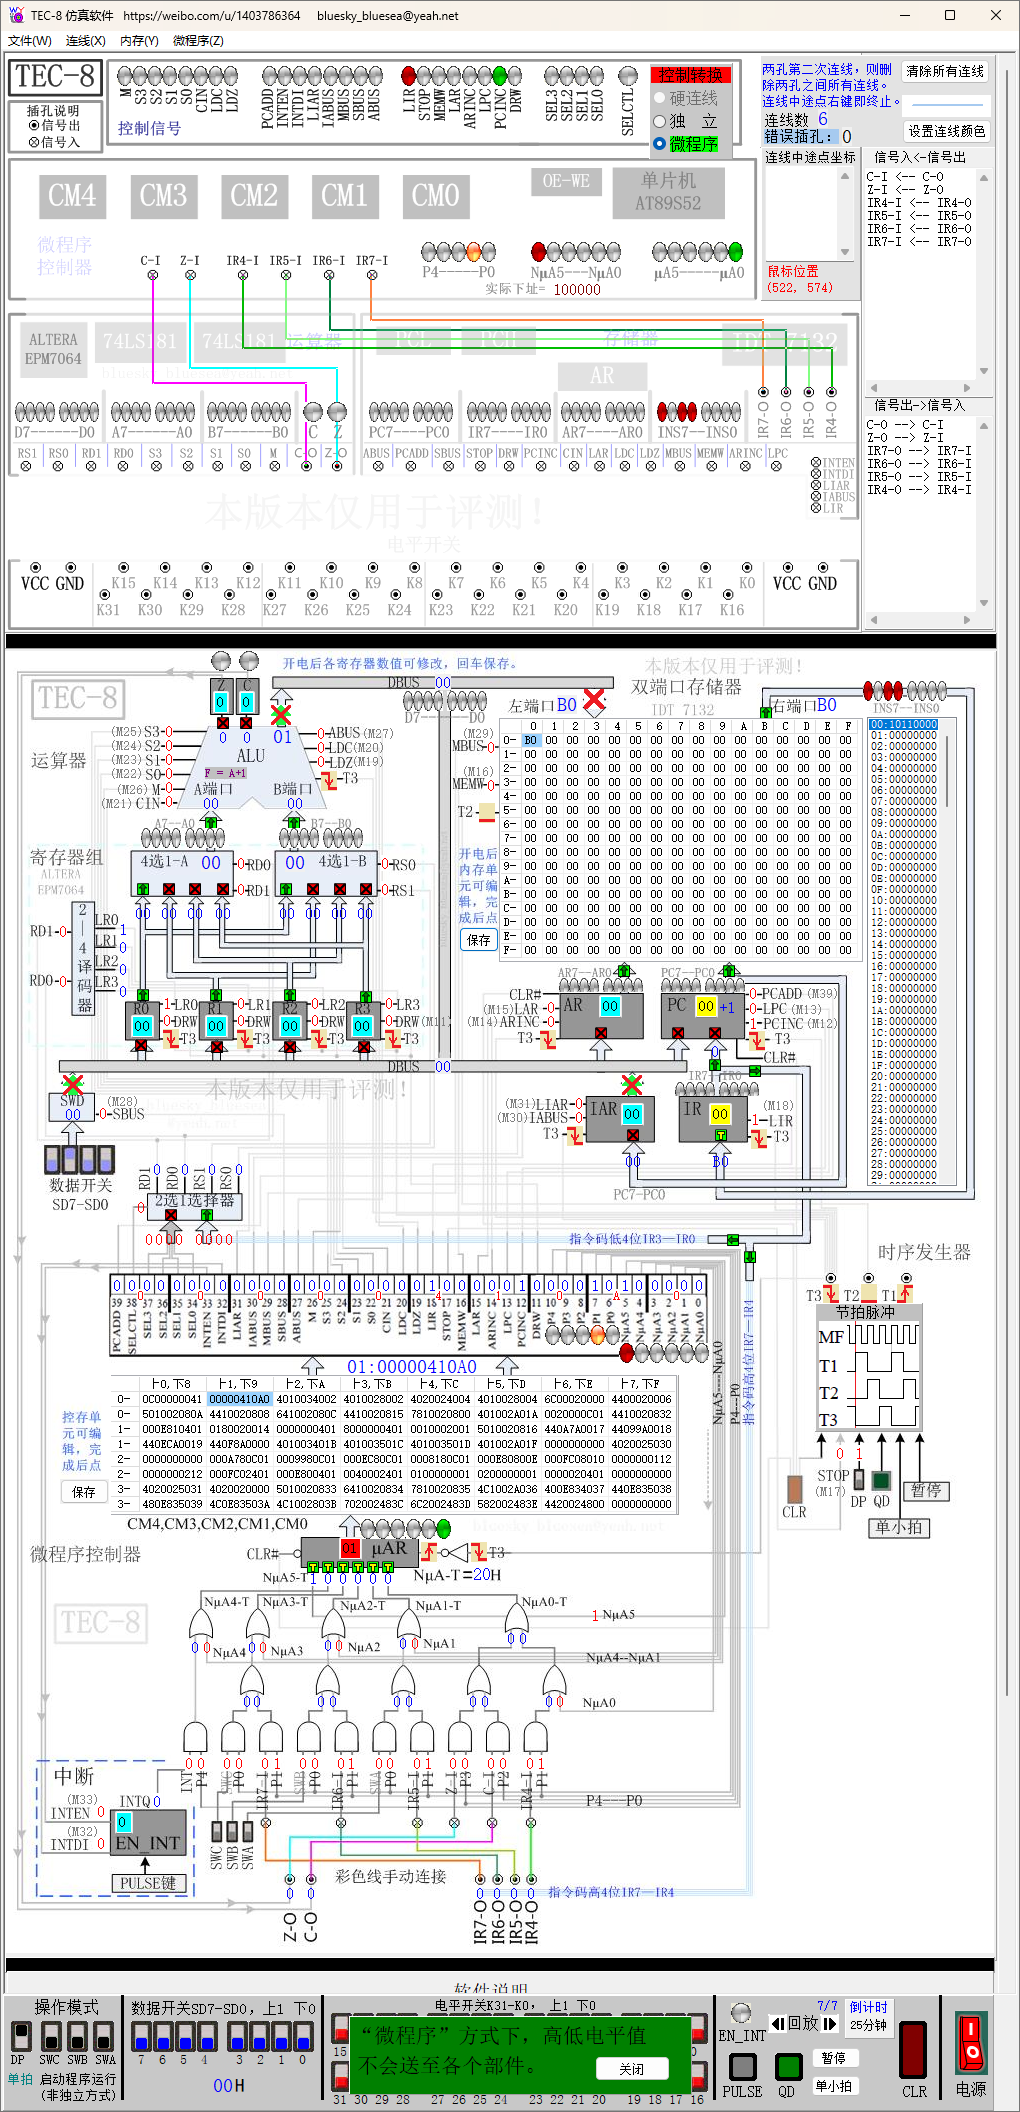
\includegraphics[width=0.3\textwidth]{screenshots/4.2.5.2.png}
    }
    \subfigure[]{
        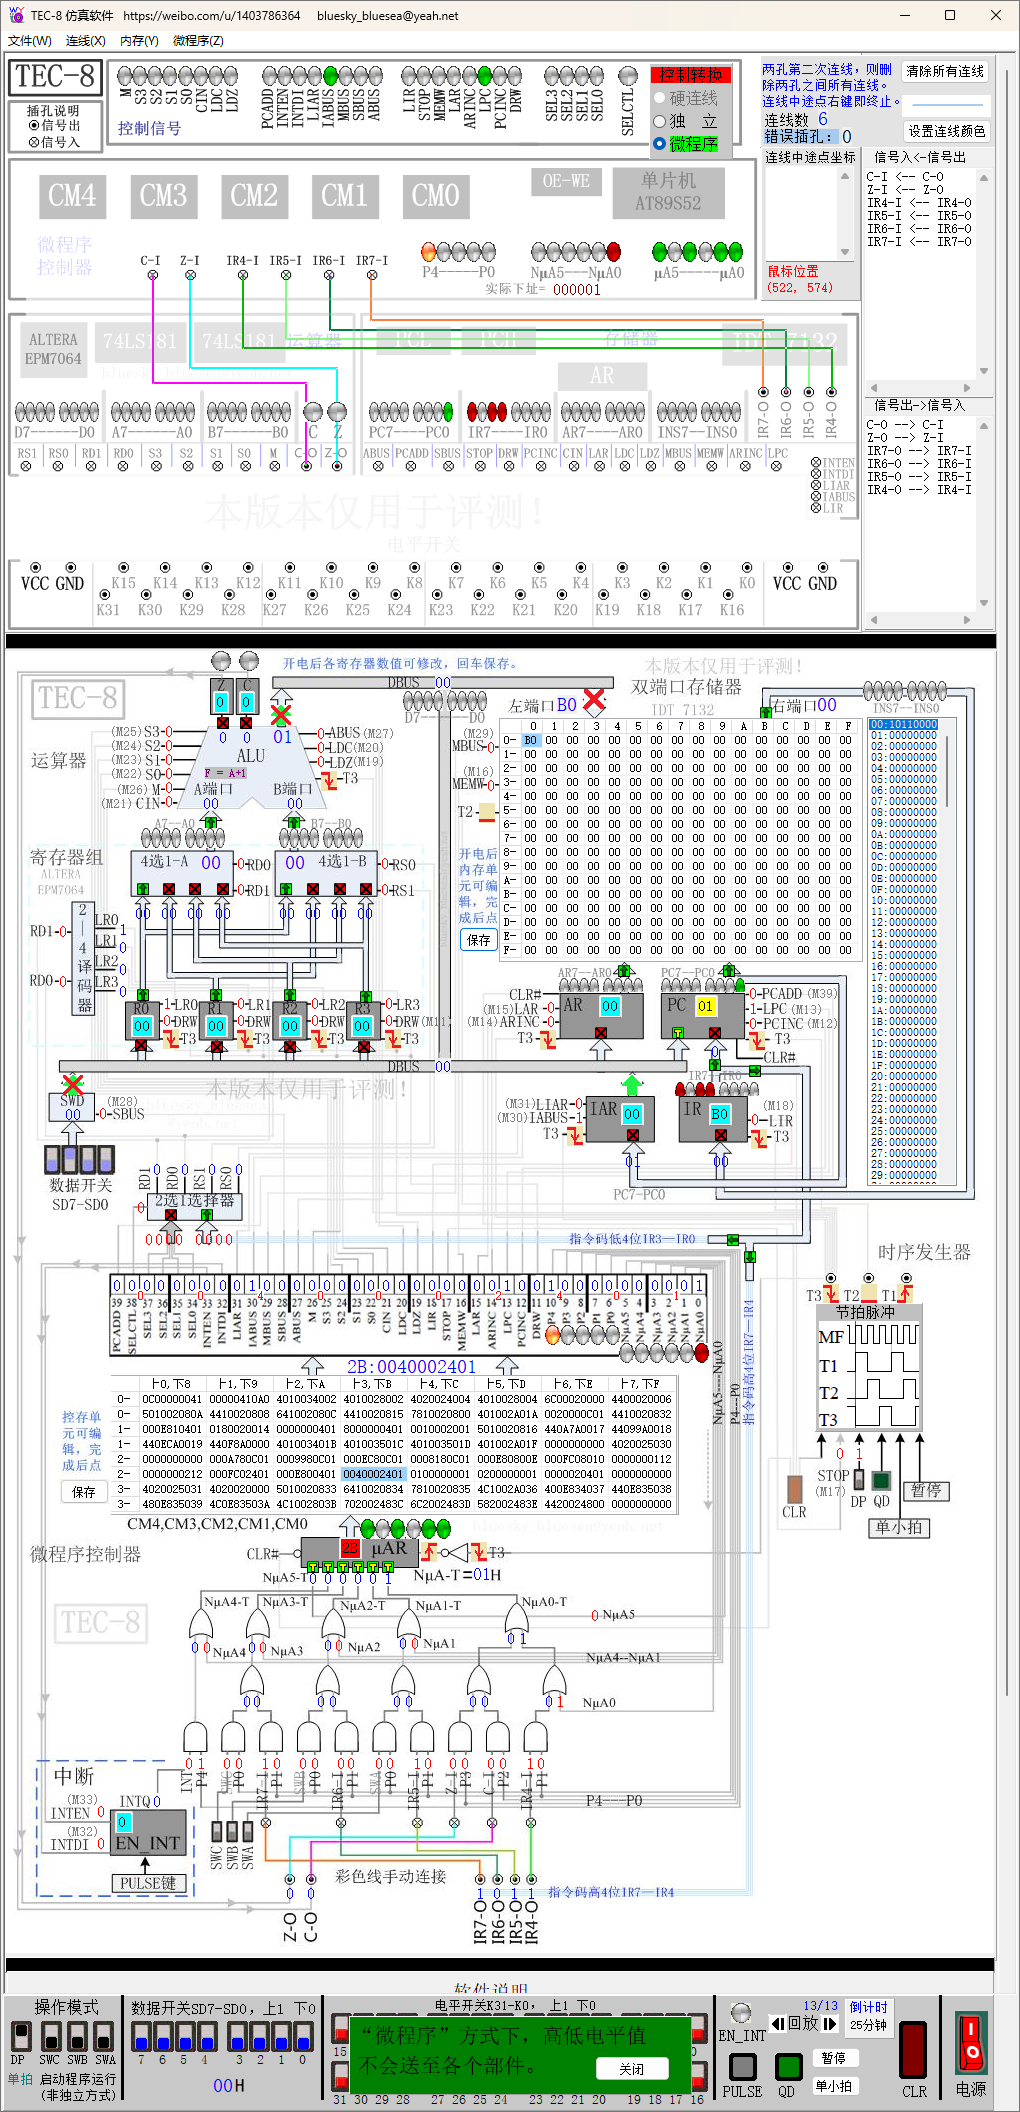
\includegraphics[width=0.3\textwidth]{screenshots/4.2.5.3.png}
    }
    \\
    \subfigure[]{
        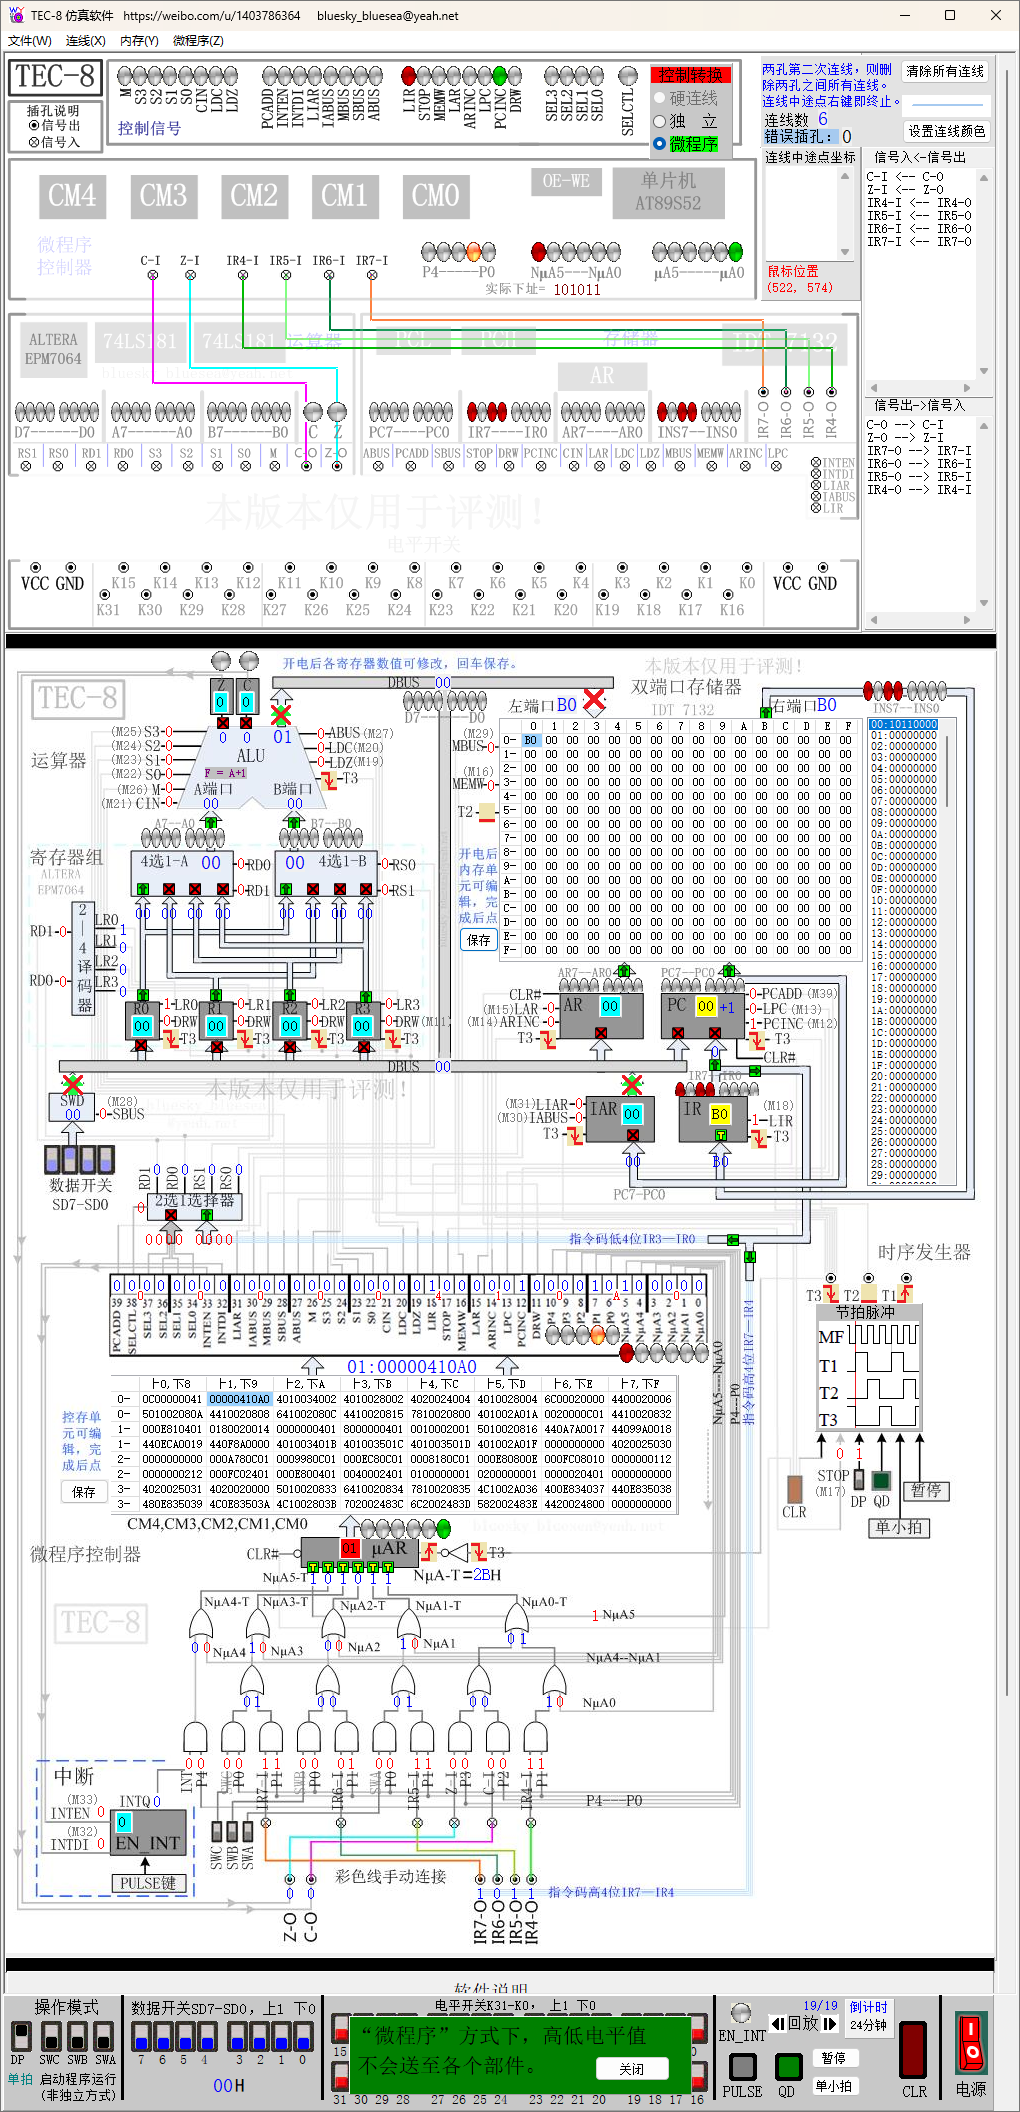
\includegraphics[width=0.3\textwidth]{screenshots/4.2.5.4.png}
    }
    \subfigure[]{
        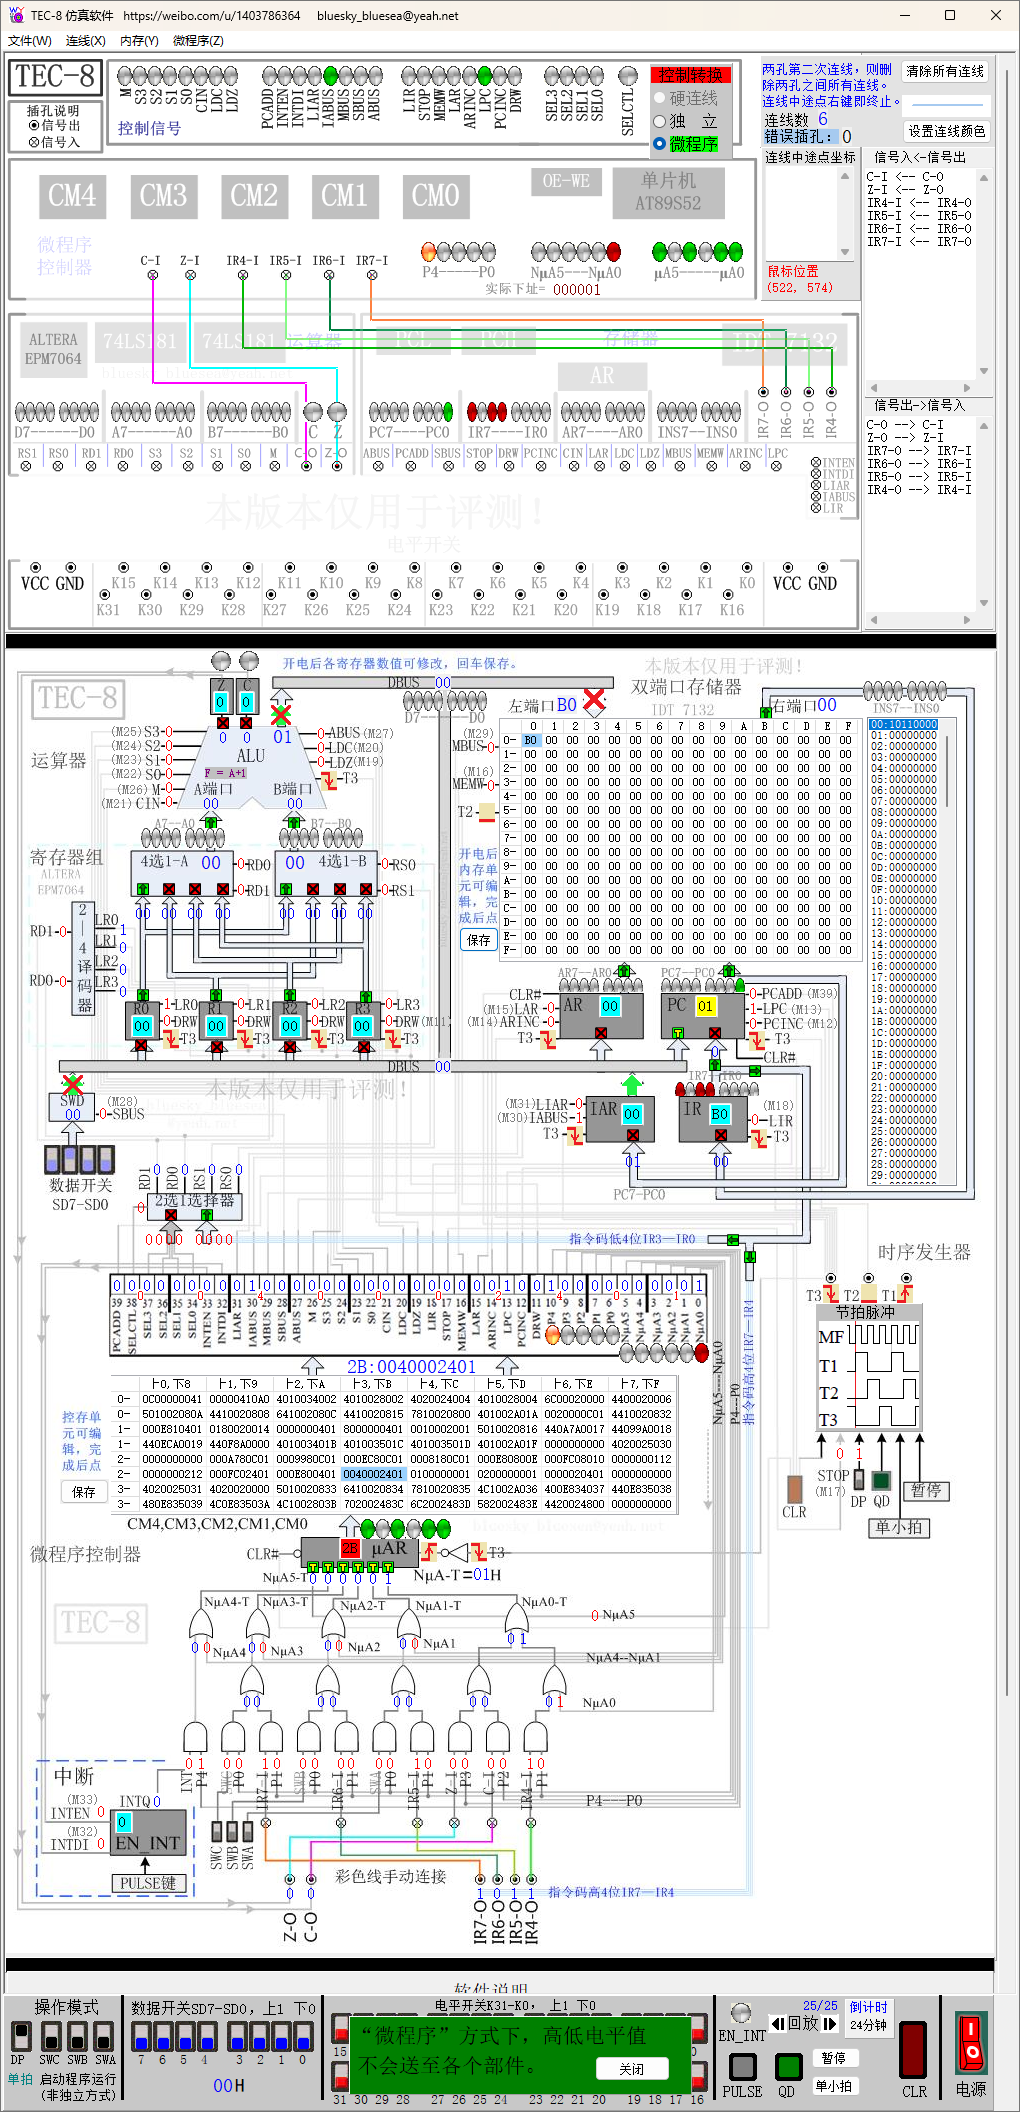
\includegraphics[width=0.3\textwidth]{screenshots/4.2.5.5.png}
    }
    \subfigure[]{
        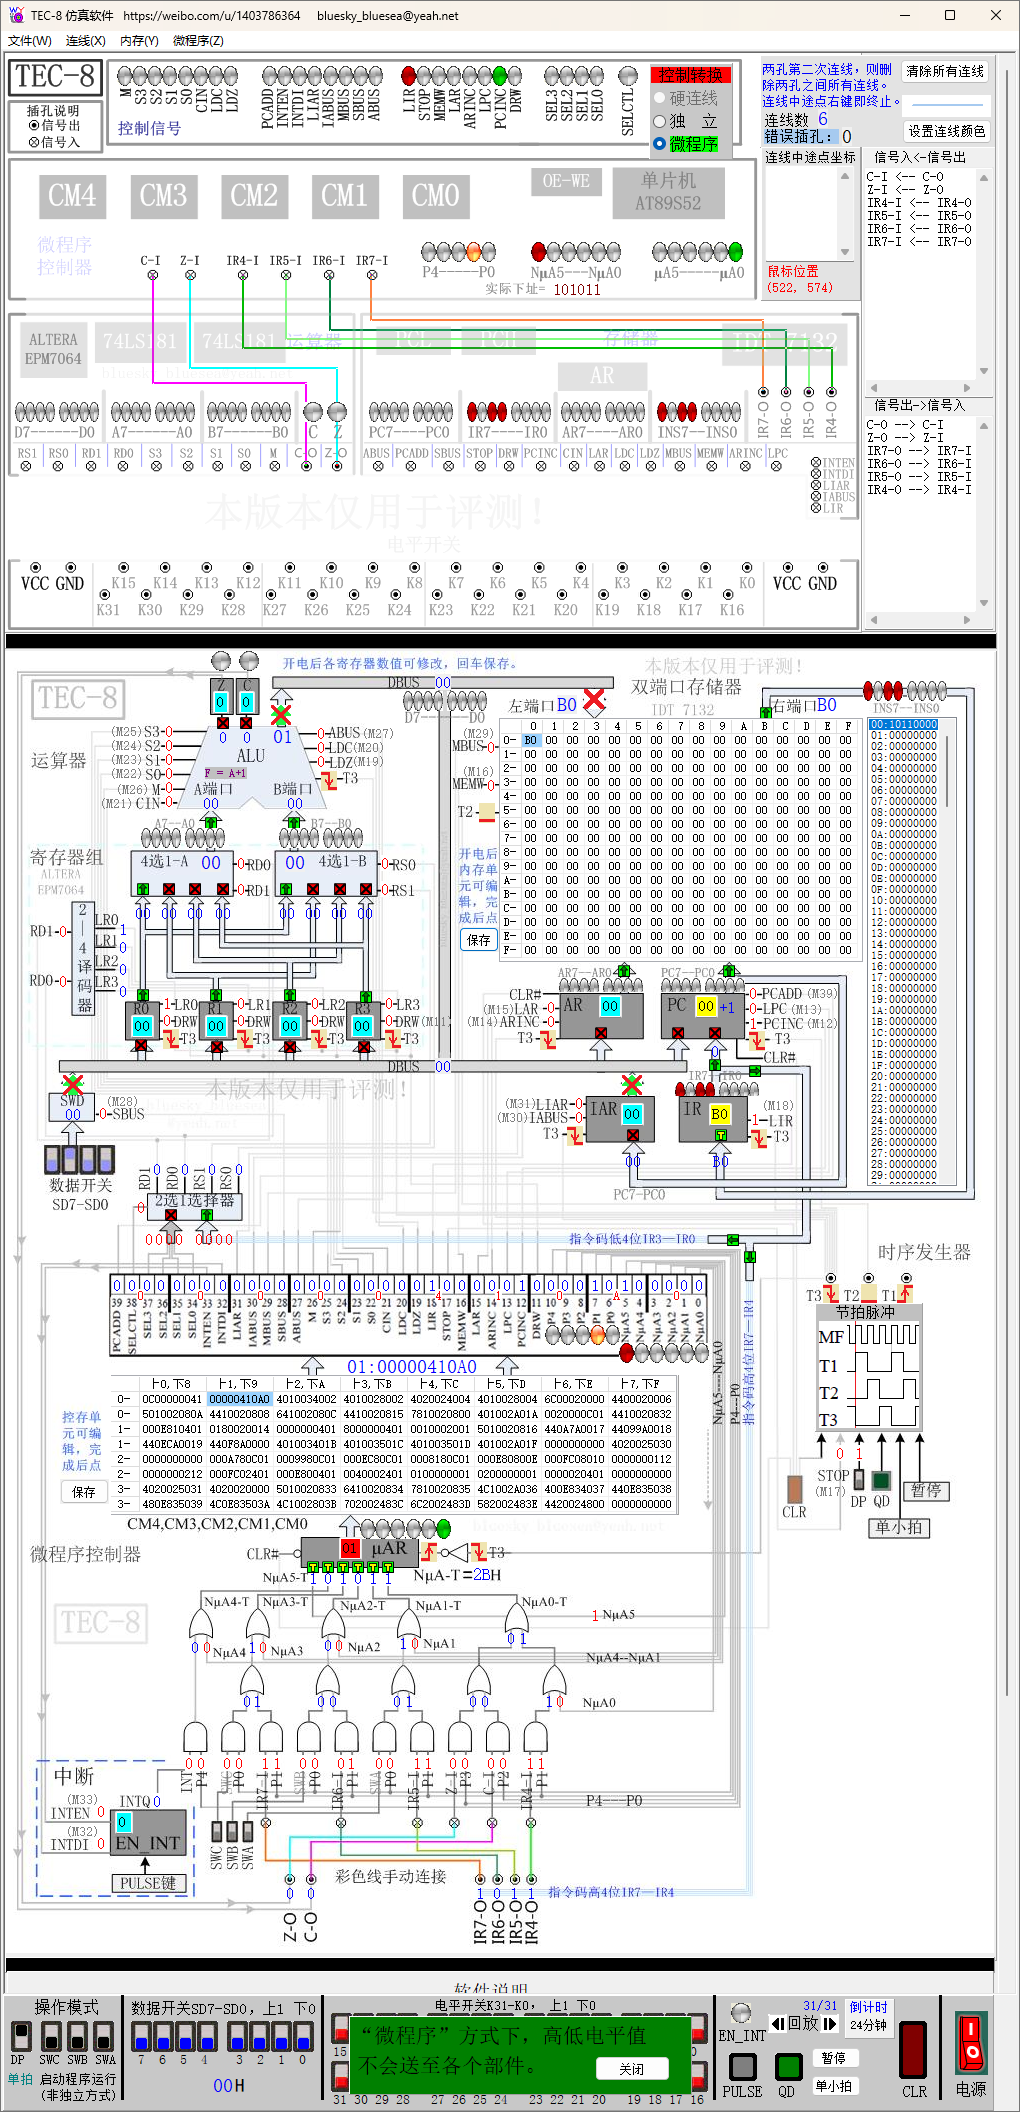
\includegraphics[width=0.3\textwidth]{screenshots/4.2.5.6.png}
    }
    \caption{中断返回}
    \label{fig: iret}
\end{figure}

\begin{figure}[htbp]
    \centering
    \subfigure[]{
        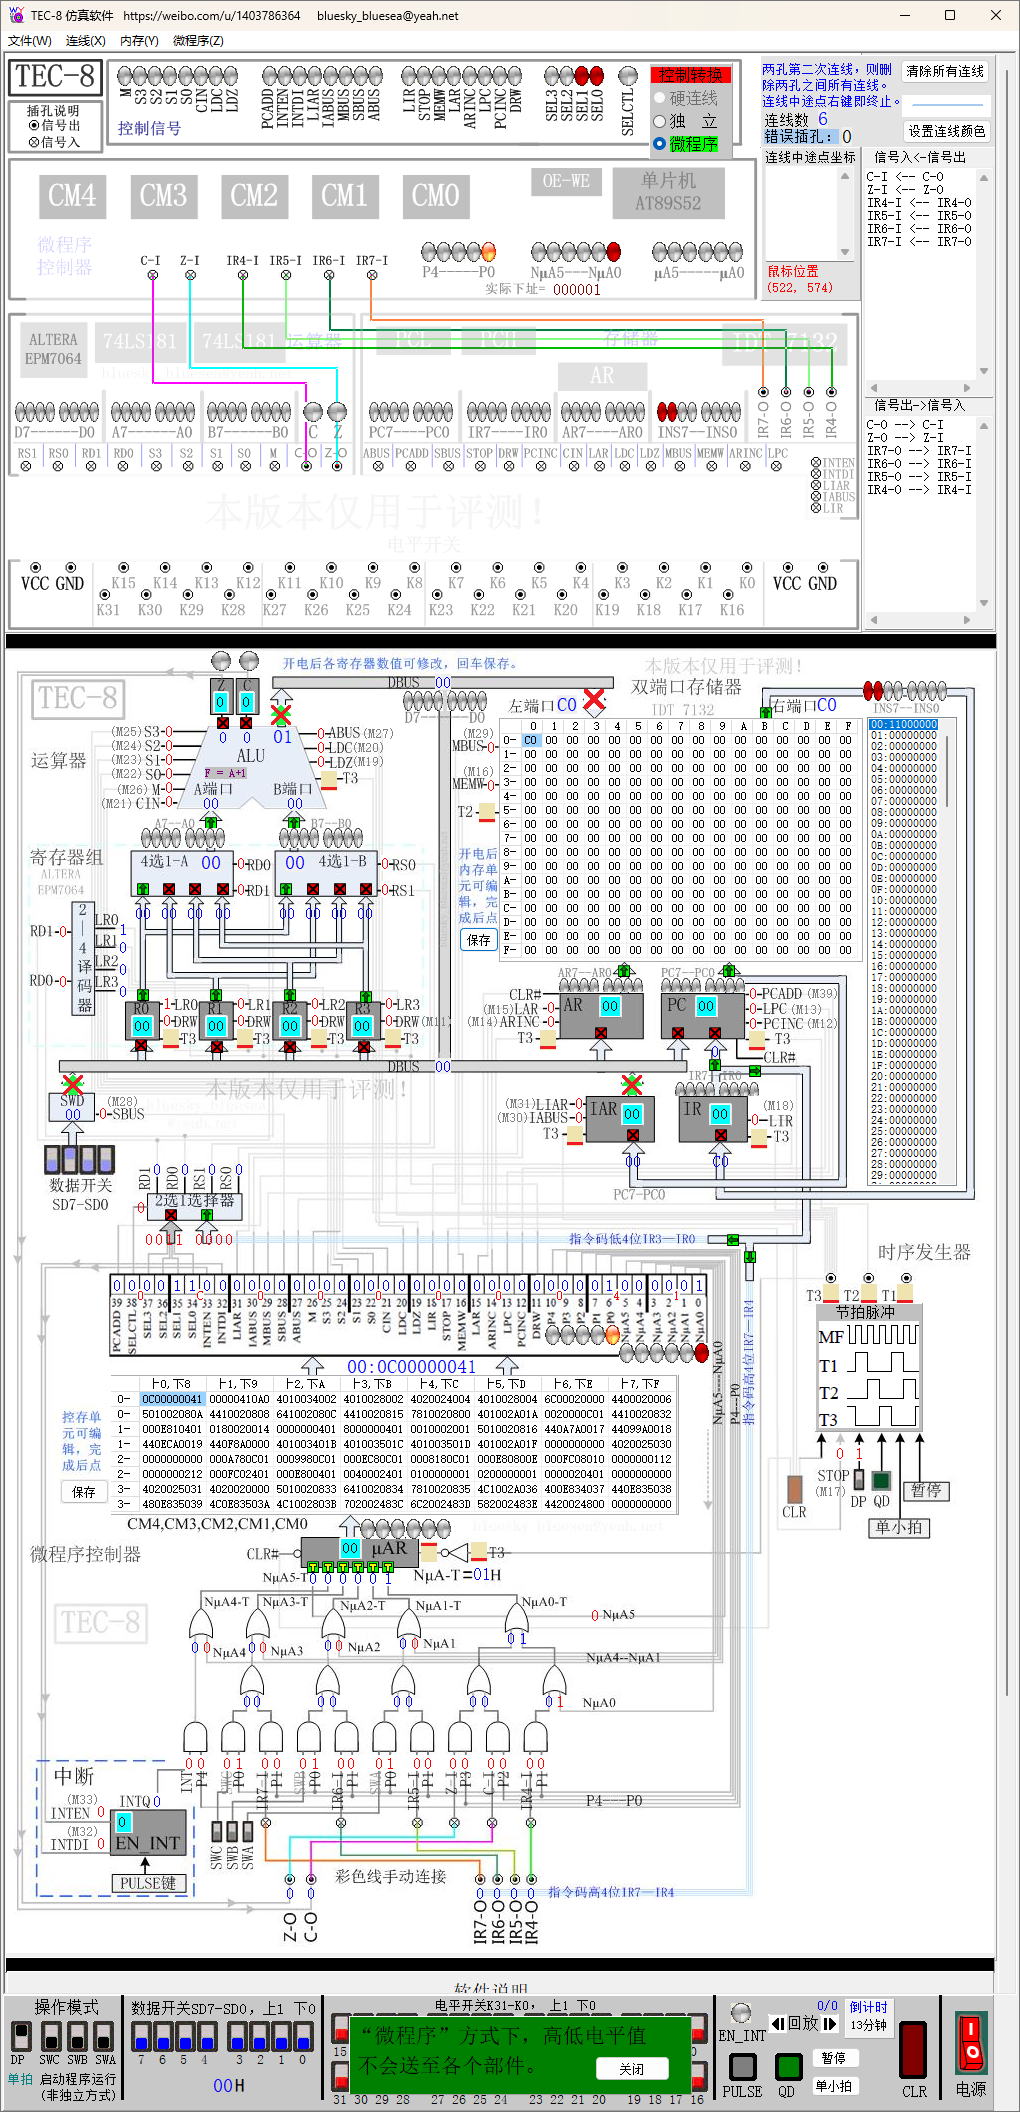
\includegraphics[width=0.3\textwidth]{screenshots/4.2.6.1.png}
    }
    \subfigure[]{
        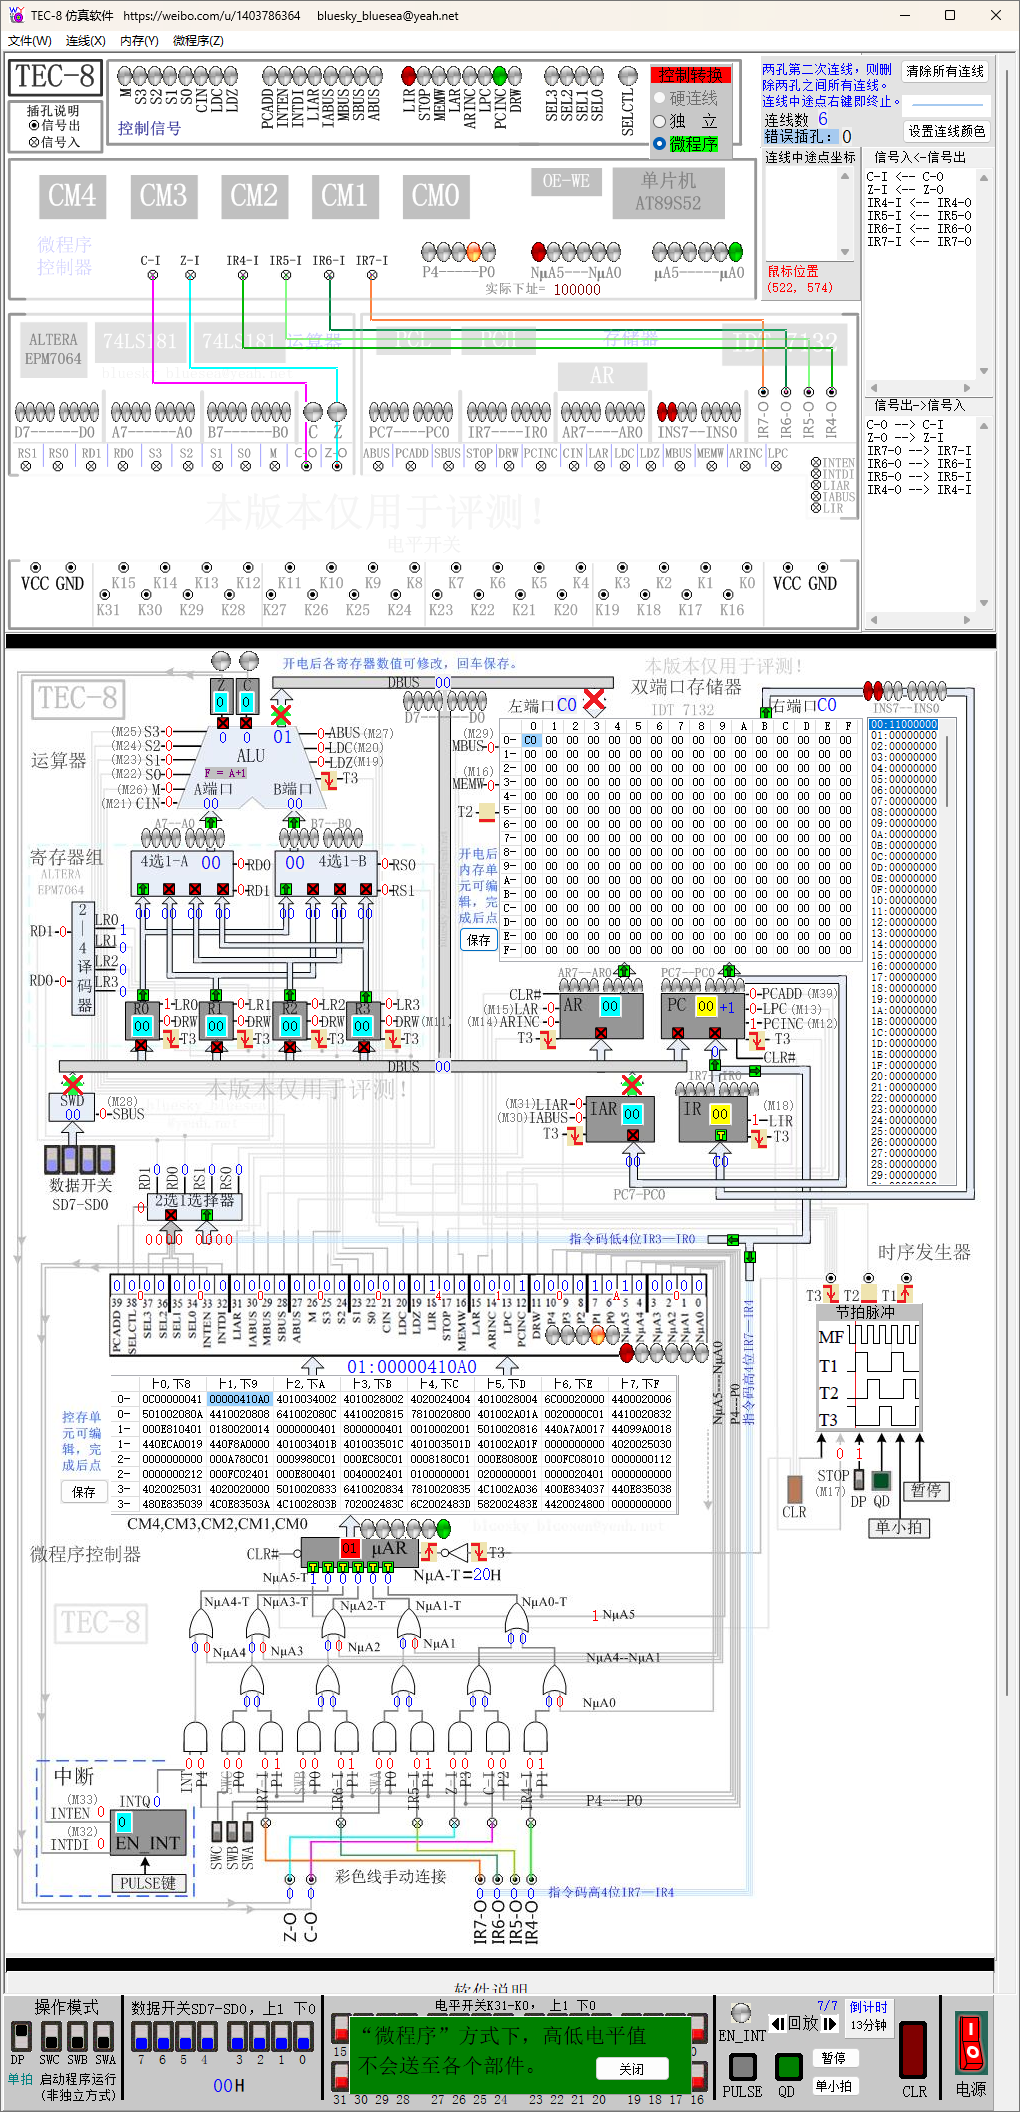
\includegraphics[width=0.3\textwidth]{screenshots/4.2.6.2.png}
    }
    \\
    \subfigure[]{
        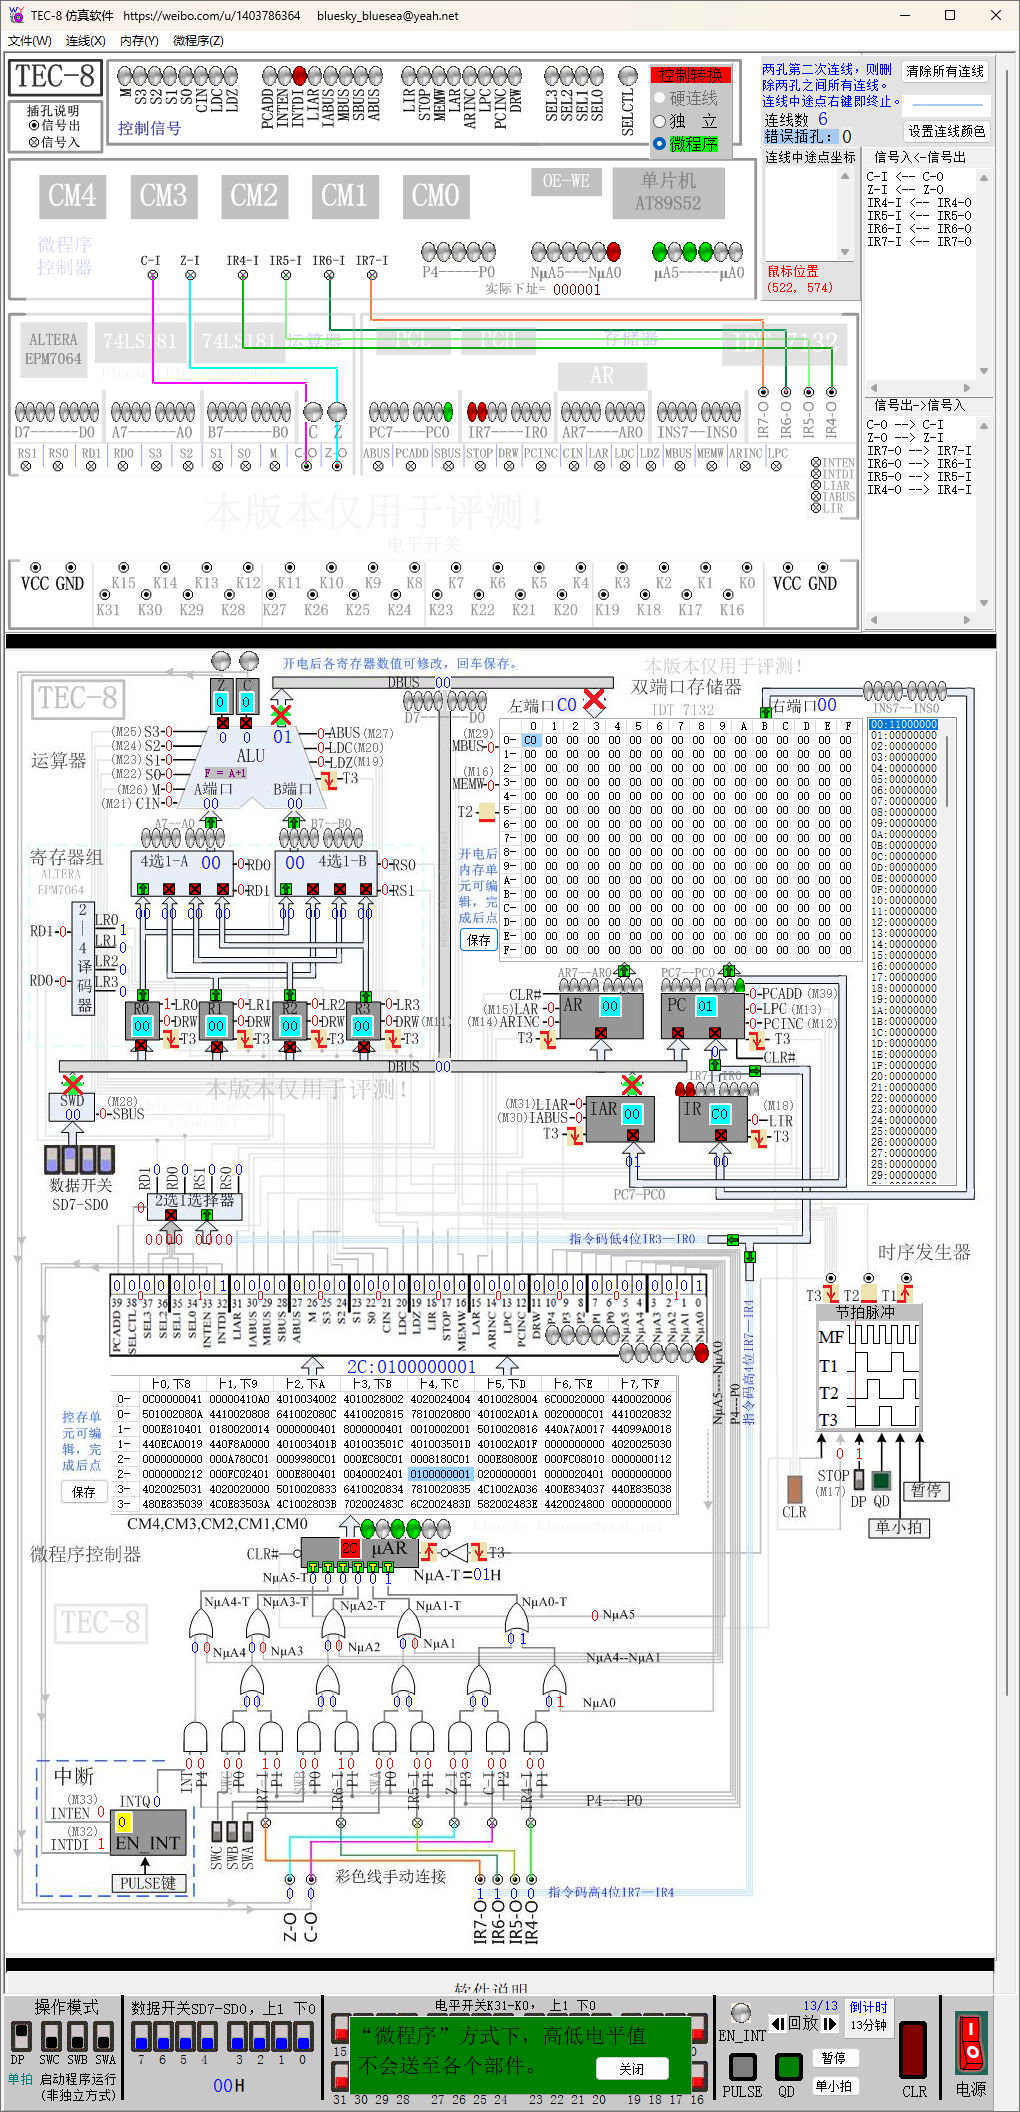
\includegraphics[width=0.3\textwidth]{screenshots/4.2.6.3.png}
    }
    \subfigure[]{
        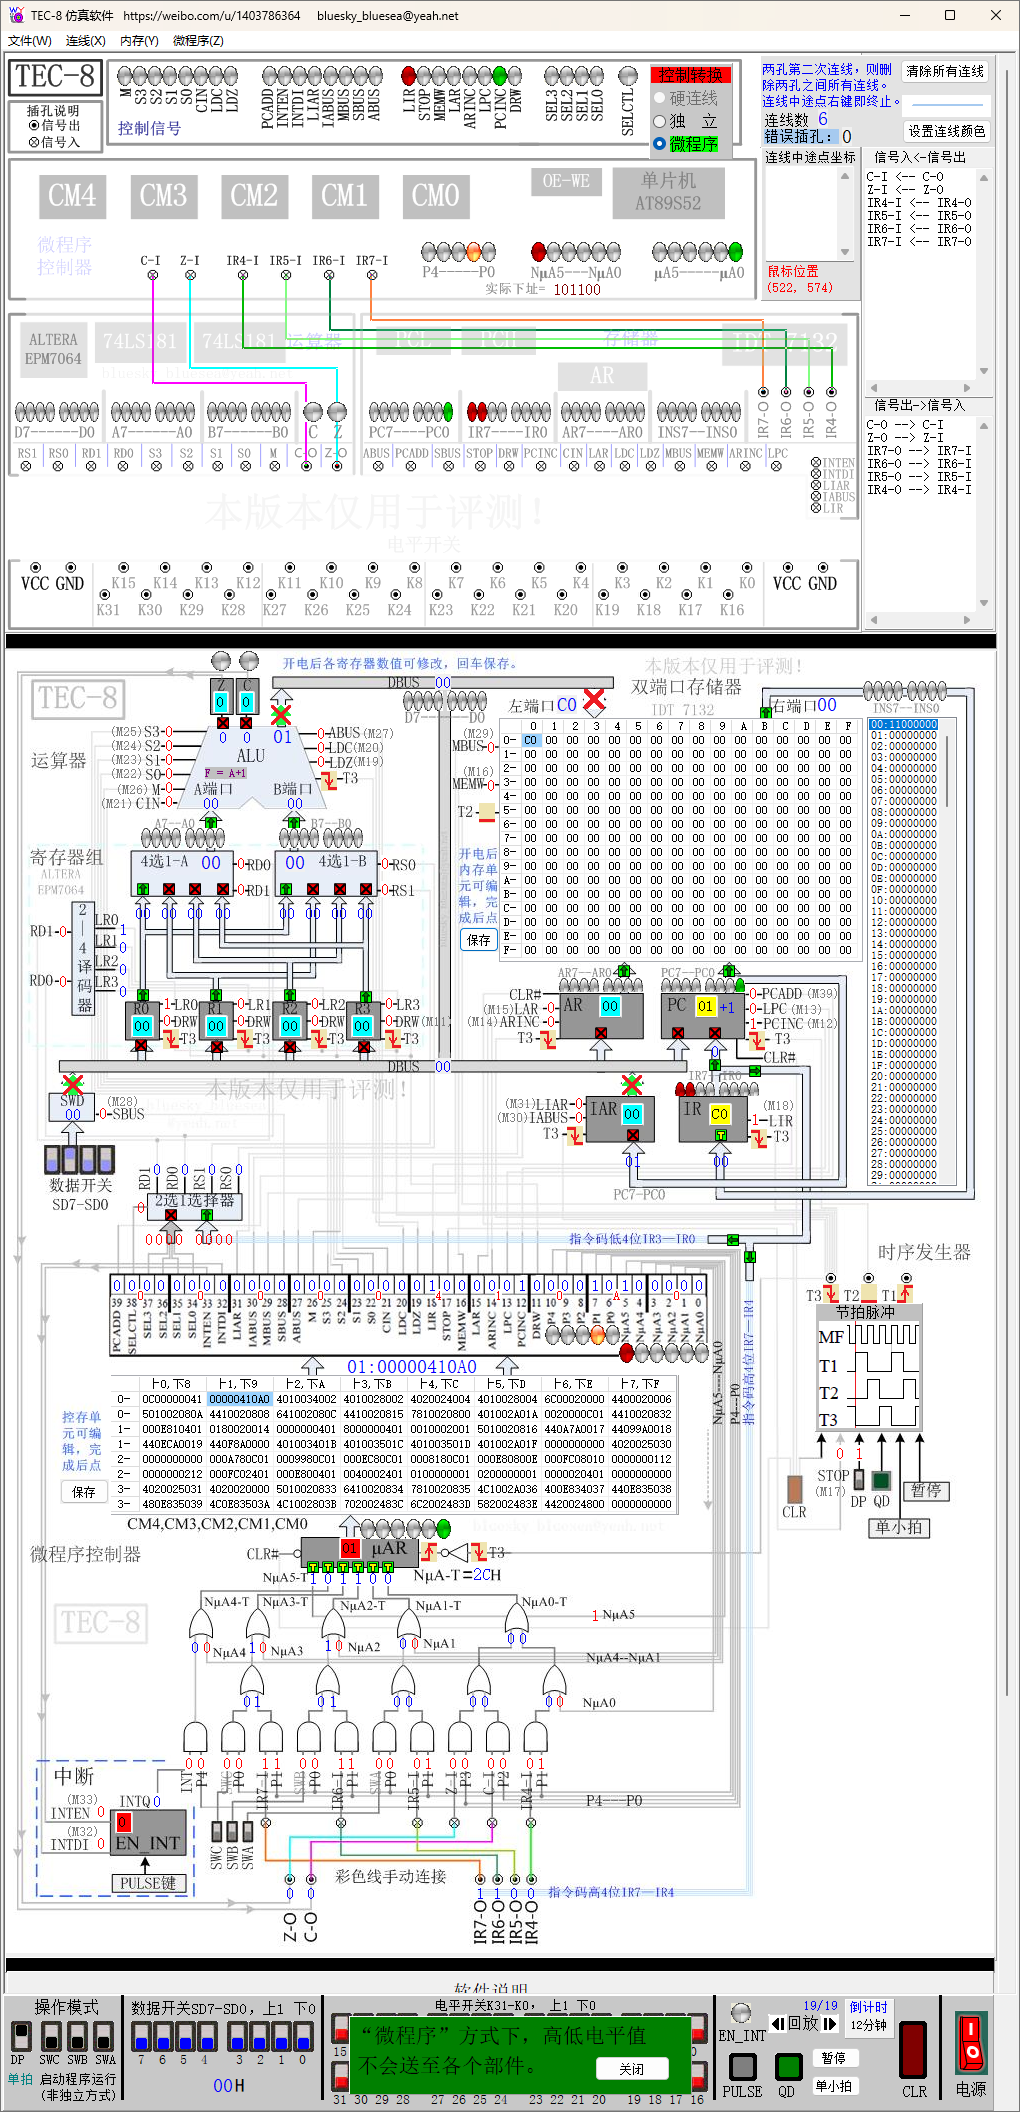
\includegraphics[width=0.3\textwidth]{screenshots/4.2.6.4.png}
    }
    \caption{开中断}
    \label{fig: di}
\end{figure}

\begin{figure}[htbp]
    \centering
    \subfigure[]{
        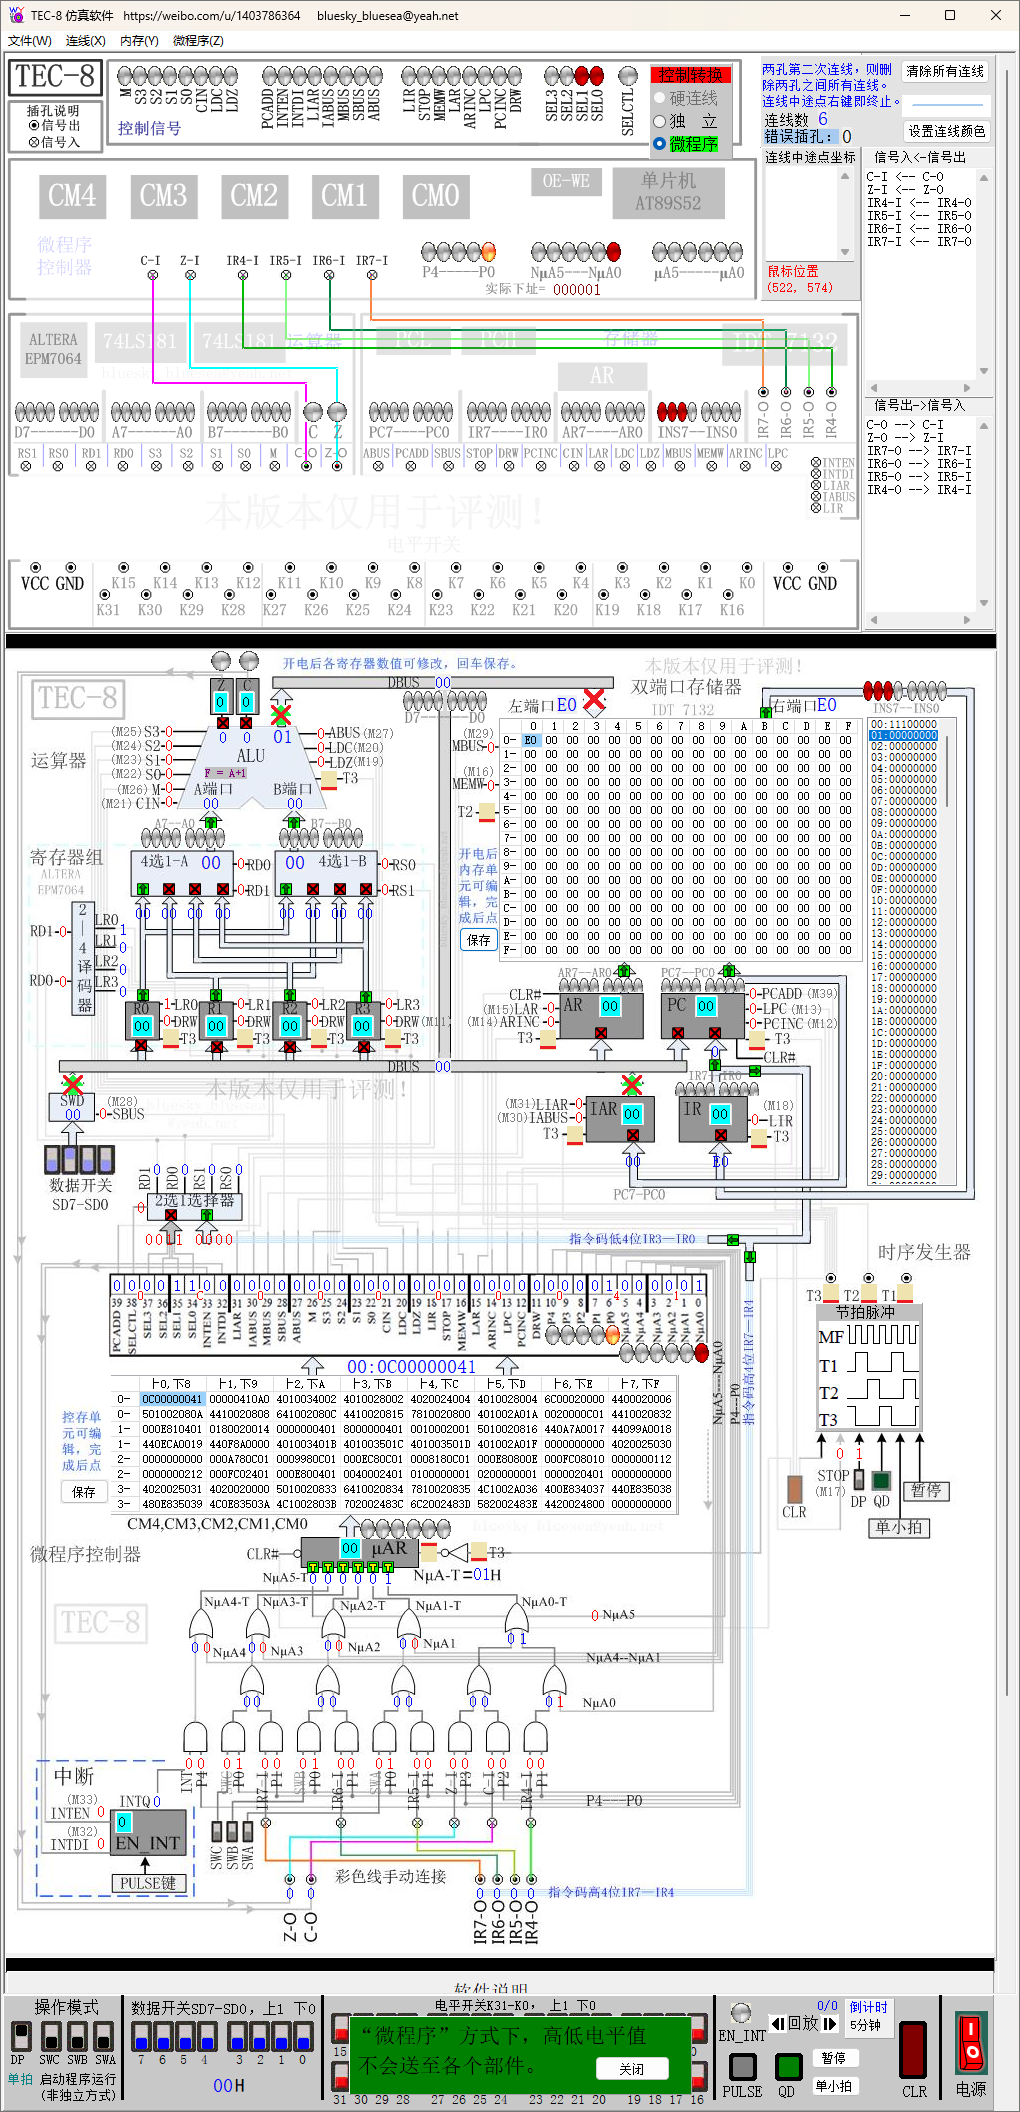
\includegraphics[width=0.3\textwidth]{screenshots/4.2.7.1.png}
    }
    \subfigure[]{
        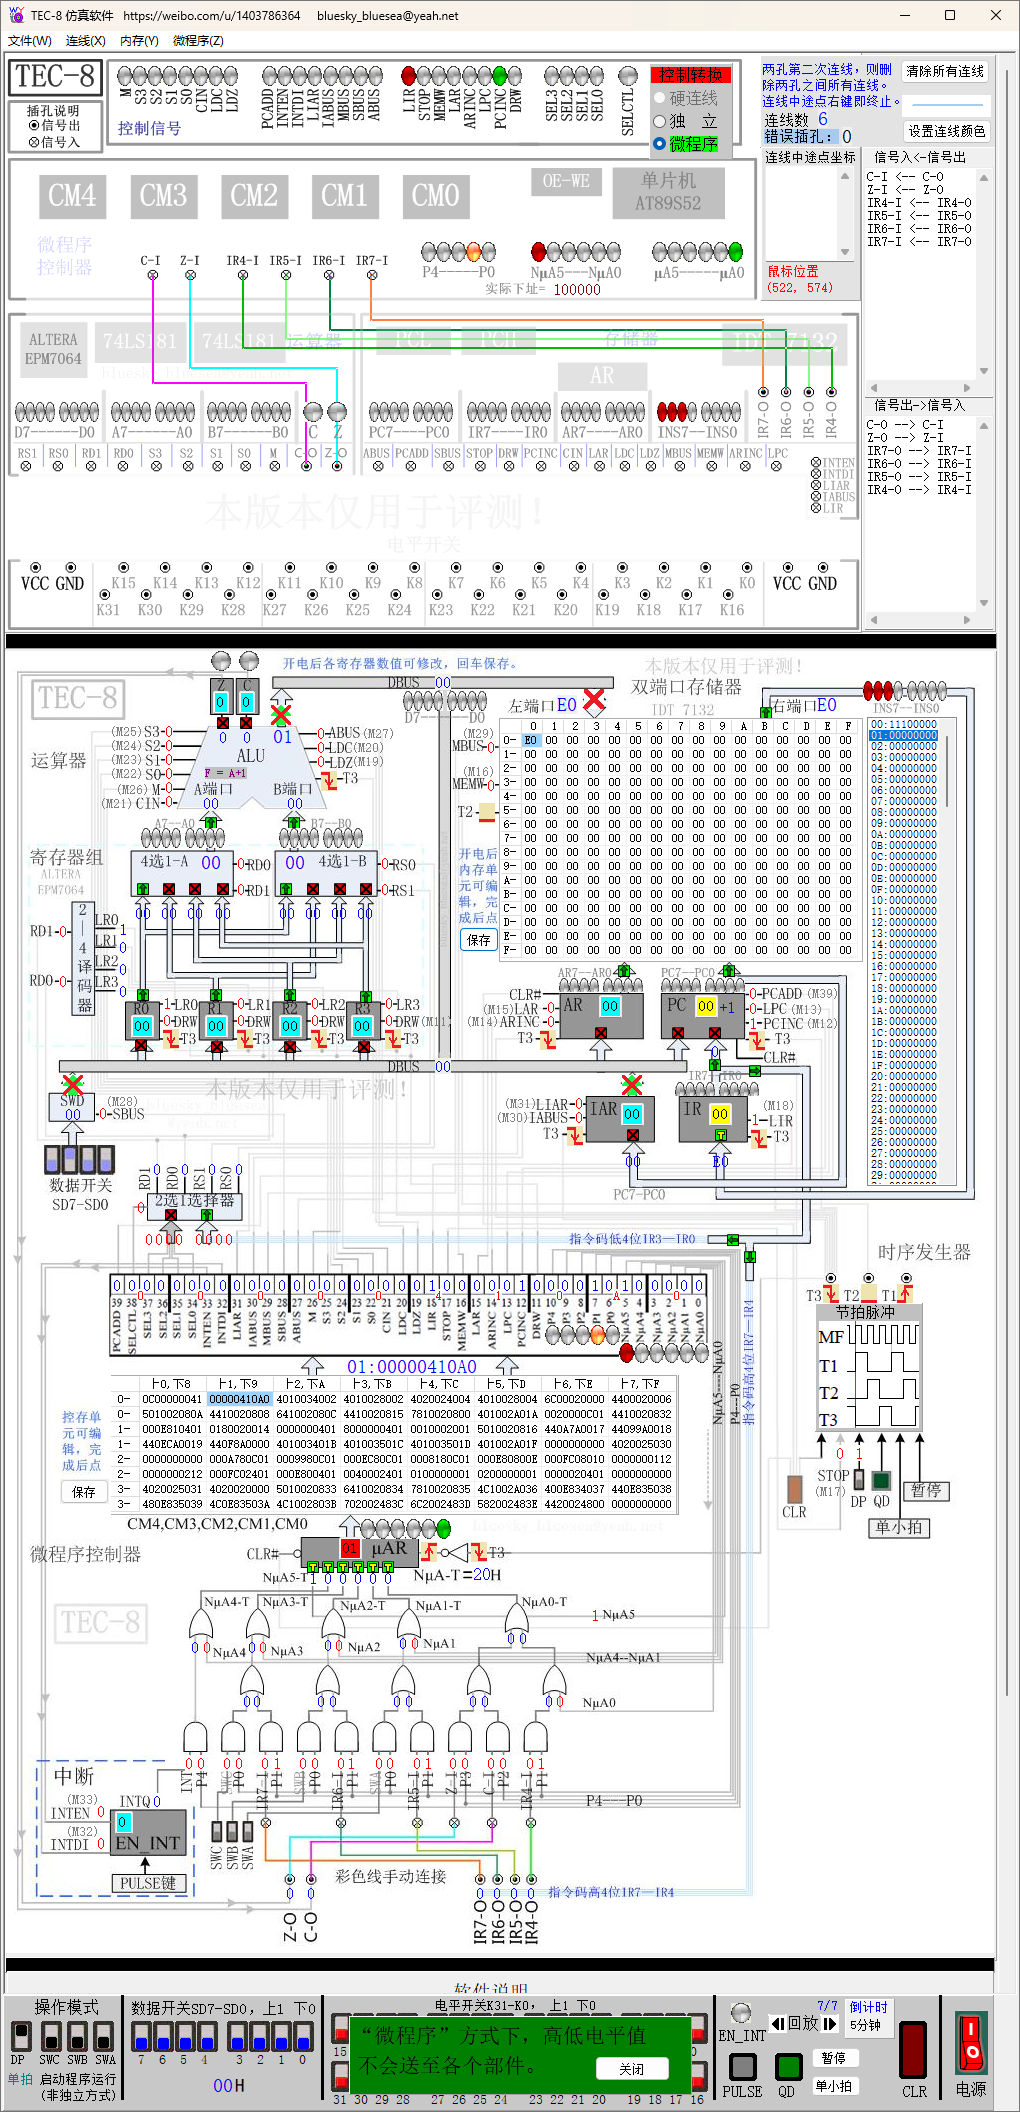
\includegraphics[width=0.3\textwidth]{screenshots/4.2.7.2.png}
    }
    \\
    \subfigure[]{
        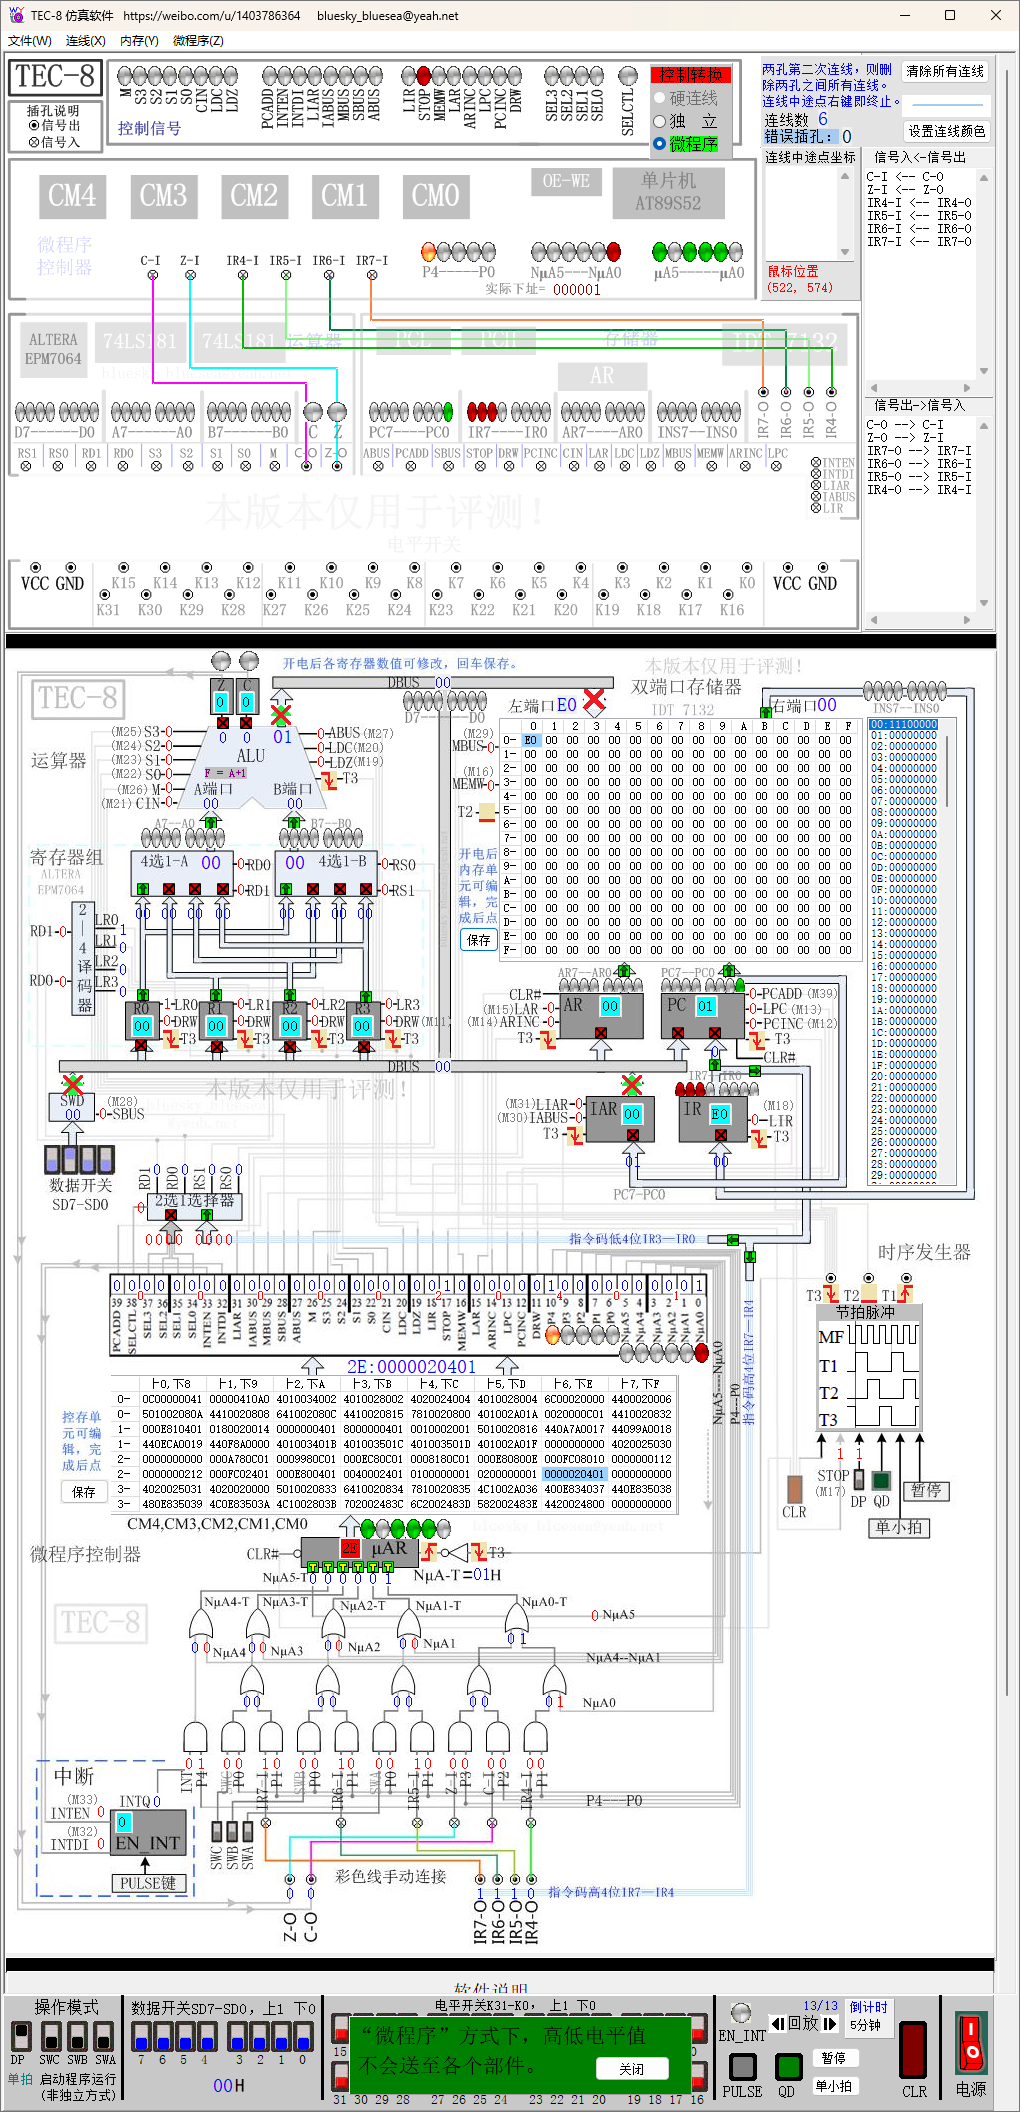
\includegraphics[width=0.3\textwidth]{screenshots/4.2.7.3.png}
    }
    \subfigure[]{
        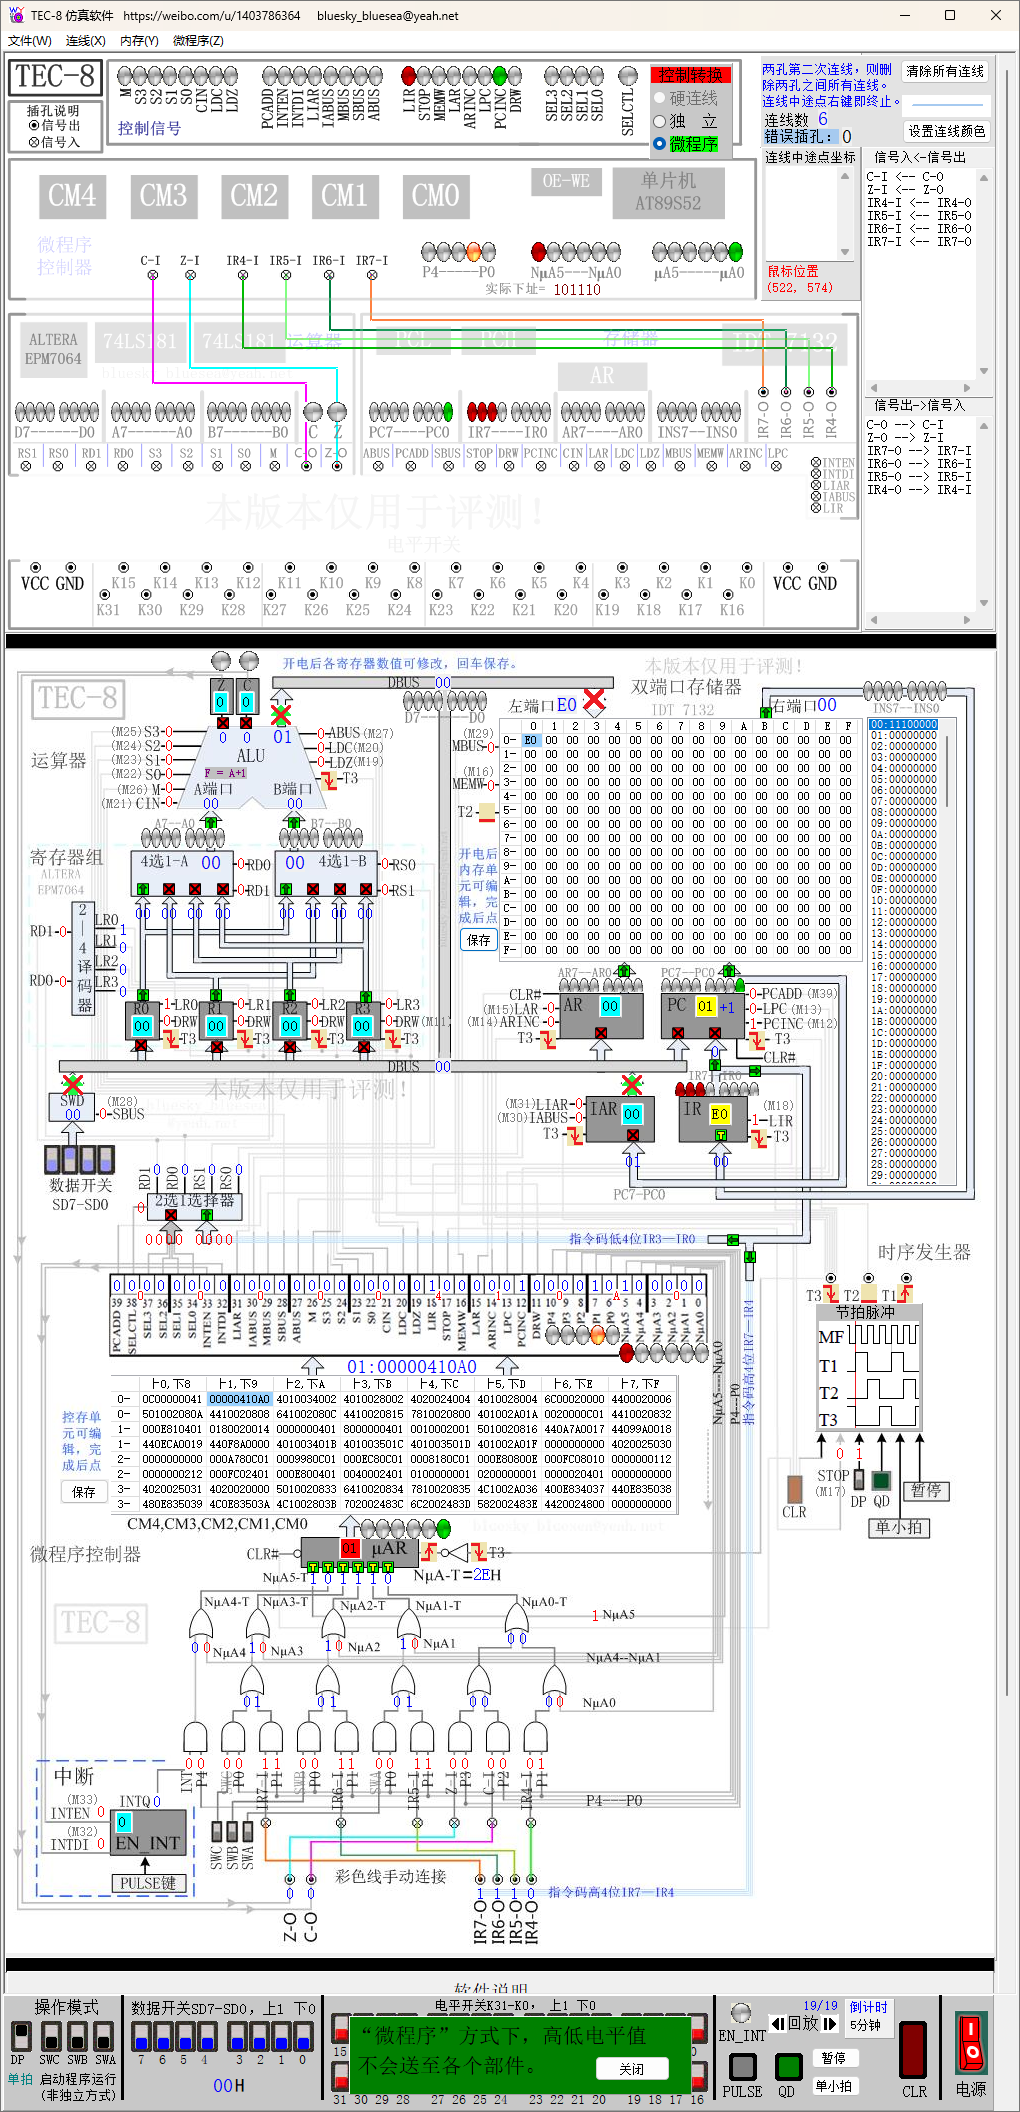
\includegraphics[width=0.3\textwidth]{screenshots/4.2.7.4.png}
    }
    \caption{关中断}
    \label{fig: ei}
\end{figure}

\end{document}